%input macros (i.e. write your own macros file called MacroFile1.tex)
%\include{Macros/MacroFile1}
 \documentclass[oneside,12pt]{Classes/CUEDthesisPSnPDF}

\newcommand{\mytitle}{Sitewise error and constraint in mammalian comparative
 genomics}

\ifpdf
    \pdfinfo { /Title  (Greg's Awesome Thesis)
               /Creator (TeX)
               /Producer (pdfTeX)
               /Author (Gregory Jordan greg@ebi.ac.uk)
               /CreationDate (D:20100930000000)  %format D:YYYYMMDDhhmmss
               /ModDate (D:20030815213532)
               /Subject (Comparative Genomics)
               /Keywords (PhD, Thesis)}
    \pdfcatalog { /PageMode (/UseOutlines)
                  /OpenAction (fitbh)  }
\fi

\title{\mytitle}

\ifpdf
  \author{\href{mailto:gjuggler@gmail.com}{Gregory Jordan}}
  \collegeordept{\href{http://www.ebi.ac.uk}{European Bioinformatics Institute}}
  \university{\href{http://www.cam.ac.uk}{University of Cambridge}}
% insert below the file name that contains the crest in-place of 'UnivShield'
  \crest{\includegraphics[width=40mm]{cam_crest.pdf}}
\else
  \author{Gregory Jordan}
  \collegeordept{European Bioinformatics Institute}
  \university{University of Cambridge}
% insert below the file name that contains the crest in-place of 'UnivShield'
  \crest{\includegraphics[bb = 0 0 292 336, width=30mm]{UnivShield}}
\fi
%
% insert below the file name that contains the crest in-place of 'UnivShield'
% \crest{\IncludeGraphicsW{UnivShield}{40mm}{14 14 73 81}}
%
%\renewcommand{\submittedtext}{change the default text here if needed}
\degree{Doctor of Philosophy}
\degreedate{September 29, 2011}

% turn of those nasty overfull and underfull hboxes
\hbadness=10000
\hfuzz=50pt

% Put all the style files you want in the directory StyleFiles and usepackage like this:
\usepackage{hyphenat}
\usepackage{Styles/bibunits}
\usepackage[small]{caption}
\usepackage{xspace,bm,amsmath,amssymb}
\usepackage{Styles/watermark}
\usepackage{multirow}
\usepackage{threeparttable}
\usepackage{array}
\usepackage{booktabs}
\usepackage{rotating}
\usepackage{pdflscape}
\usepackage{longtable}
\usepackage[table]{xcolor}
%\usepackage[colorinlistoftodos, textwidth=4cm, shadow]{todonotes}
\usepackage{a4wide}
\usepackage[printonlyused]{acronym}

% Comment out the next line to get single spacing
\onehalfspacing
%\renewcommand{\baselinestretch}{1.8}

\renewcommand\floatpagefraction{.9}
\renewcommand\topfraction{.95}
\renewcommand\bottomfraction{.95}
\renewcommand\textfraction{.2}
\setcounter{totalnumber}{50}
\setcounter{topnumber}{50}
\setcounter{bottomnumber}{50}

\begin{document}

%\language{english}

% A page with the abstract on including title and author etc may be
% required to be handed in separately. If this is not so, then comment
% the below 3 lines (between '\begin{abstractseparte}' and 
% 'end{abstractseparate}'), normally like a declaration ... needs some more
% work, mind as environment abstracts creates a new page!
% \begin{abstractseparate}
%   \input{Abstract/abstract}
% \end{abstractseparate}


% Using the watermark package which is in StyleFiles/
% and to remove DRAFT COPY ONLY appearing on the top of all pages comment out below line
%\watermark{DRAFT COPY ONLY}

\maketitle

%set the number of sectioning levels that get number and appear in the contents
\setcounter{secnumdepth}{1}
\setcounter{tocdepth}{1}

\frontmatter % book mode only
% Thesis Dedictation ---------------------------------------------------

\begin{dedication} %this creates the heading for the dedication page

This thesis is dedicated to...

\end{dedication}

\begin{acknowledgements}      %this creates the heading for the acknowlegments

First and foremost I would like to thank Nick Goldman, who supervised
my Ph.D. research at the EBI. I arrived with little knowledge and even
less experience; it is a testament to Nick's patience, encouragement,
and unequivocal support that I arrived at the other end some sort of
scientist. Thanks especially for giving me the freedom to make my own
mistakes---and for having the kindness to help mend them.

For enlightening my mind and enriching my spirits at work and beyond,
I have the past, former and current members of the Goldman Group to
thank. One would have some difficulty casting a more insightful,
helpful, and playfully skeptical ensemble. The characters, in order of
appearance: Tim, Ari, Martin, Fabio, Jacky, Stefan, Emeric, Botond,
and Hazel (plus the cameos and guest appearances).

My work and my scientific growth have benefitted greatly from fruitful
discussions and productive collaborations with several others who got
caught in my academic web. My thesis advisory committee (Ewan Birney,
Nick Mundy, and Jan Korbel) provided useful feedback and well-tempered
advice; members of the Ensembl Compara team (Albert Vilella, Javier
Herrero) kindly introduced me to their systems and taught me
invaluable ``farming techniques''; and other collaborators (including
Stephen Montgomery, Aylwyn Scally, Tim O'Connor, Amalio Telenti, David
Aanansen and the members of the Mammalian Genome Project Consortium)
have together taught me innumerable lessons about how to do good work
and play nice with others.

To my family, I owe everything for their love and support over the
past years. I couldn't have dreamt of feeling so close to home while
living thousands of miles away. Sure, Skype helped, but it was a
feeling much more magical than the Internet that kept me close.

Throughout the years I've been blessed with great friends, who
together made sure life in Cambridge never lost its lustre. My adopted
Gates ``family'' embraced me with entertaining dinners, exciting trips
and a new bunch of lifelong friends. Juggling pals Ben and Guy allowed
me a curious peek into the world of May ball entertainment. And my
amazing housemates, the fearless tenants of the pink house on
Coleridge Road---Niko, Lesley, Loizos, Jan, Felix, Tom and Karolina
through the years---have always been there when I most needed to
laugh, commisserate, eat good food, or enjoy yet another alphabetical
party.

Finally, the EBI Predocs \& Friends have been there all along, a core
to my life in so many ways. The gang of 2007 predocs---Michele,
Markus, Adam, Diva, Julia and Judith---have been constant companions
from Heidelberg to Cambridge, as well as reliable scientists, friends,
and travelers on our various acronymic holidays. To all the others, I
am thankful for the never-ending mailing list hijinks, the 24-hour
support network (for computers and for life) and the endless good
cheer. It's a rare bunch that can keep you looking forward to what's
next even after four years. And I would like to extend a very special
thank-you to Anna, who as a friend and so much more has filled this
``thesis year'' of our lives with a much-needed blend of caring,
encouragement and fun.

\end{acknowledgements}

\setlength{\parskip}{\baselineskip}

\noindent This dissertation is the result of my own work and includes nothing
which is the outcome of work done in collaboration except where
specifically indicated in the text and acknowledgements.

\noindent This dissertation is not substantially the same as any I have
submitted for a degree, diploma or other qualification at any other
university, and no part has already been, or is currently being
submitted for any degree, diploma or other qualification.


\noindent This dissertation does not exceed the specified length limit
of 60,000 words as defined by the Biology Degree Committee.

\noindent \today \hfill Gregory Jordan

\setlength{\parskip}{0pt}

\begin{center}
\Large \mytitle

\large Summary
\end{center}

\hfill Gregory Jordan \\
\noindent{\today} \hfill Darwin College \\

Insight into the evolution of protein-coding genes can be gained from
the use of phylogenetic codon models. Recently sequenced mammalian
genomes and powerful analysis methods developed over the past decade
provide the potential to globally measure the impact of natural
selection on protein sequences at a fine scale. The detection of
positive selection in particular is of great interest, with relevance
to the study of host-parasite conflicts, immune system evolution and
adaptive differences between species. This thesis examines the
performance of methods for detecting positive selection first with a
series of simulation experiments, and then with two empirical studies
in mammals and primates.

Our ability to make confident estimates of the prevalence of positive
selection in proteins has been hampered to some extent by uncertainty
regarding the level of false positives resulting from alignment
error. To this end, I conduct a simulation study to estimate the rate
of false positive results attributable to alignment error. A variety
of aligners and alignment filtering methods are compared, showing a
striking difference between aligners in their tendency to produce
false positive results. Under most conditions, the best aligners tend
to produce very few false positives due to misalignment.

The rest of this thesis focuses on two genome-wide studies: an
analysis of sitewise selective pressures across 38 mammalian genomes,
and a genome-wide scan for genes with evidence of accelerated
evolution in gorilla and the African great apes. In the broader
mammalian analysis, the global distribution of sitewise evolutionary
constraint is characterized and strong evidence is presented for less
positive selection in the protein-coding genes of rodents compared to
primates and other mammalian orders. New methods are developed for
combining sitewise estimates across genes and protein-coding domains,
revealing widespread signals of positive selection in genes and
domains related to host defense and, surprisingly, centromere
binding. The African great ape analysis uses phylogenetic codon models
to identify genes which have experienced elevated evolutionary rates
in gorilla, human and chimpanzee. Similar numbers of accelerated genes
are identified in each of these genomes, and several accelerated genes
are identified in gorilla with plausible relationships to its unique
phenotypic and behavioral characteristics. Finally, genome-wide coding
alignments are used to infer genome-wide selective pressures along
each branch of the great ape tree, providing corroborating evidence of
a trend towards decreasing population sizes in the recent evolutionary
history of African great apes.


\tableofcontents

\mainmatter % book mode only


\acrodef{fpr}[FPR]{false positive rate}
\acrodef{lot}[LOT]{largely orthologous tree}
\acrodef{mpl}[MPL]{mean path length}
\acrodef{mgp}[MGP]{Mammalian Genome Project}
\acrodef{tc}[TC]{taxonomic coverage}
\acrodef{tcc}[TCC]{taxonomic coverage constraint}

\newcommand{\tocite}[2]{\draft{To cite: \citet{#1} --- #2}}


\newcommand{\TODO}[1]{\textcolor{red}{TODO} \todo{#1}\xspace}
\newcommand{\draft}[1]{\textcolor{gray}{[#1]}\xspace}
%\newcommand{\todo}{\textcolor{red}{TO-DO}\xspace}

\newcommand{\gene}[1]{\emph{#1}}
\newcommand{\species}[1]{\emph{#1}}

% Intro
\newcommand{\syn}{synonymous\xspace}
\newcommand{\nsyn}{non-synonymous\xspace}

\newcommand{\sw}{sitewise\xspace}
\newcommand{\ml}{maximum likelihood\xspace}

\newcommand{\slr}{SLR\xspace}
\newcommand{\pamlTwo}{PAML M2\xspace}
\newcommand{\pamlEight}{PAML M8\xspace}

\newcommand{\fpr}{FPR\xspace}
\newcommand{\pss}{PSS\xspace}
\newcommand{\psg}{PSG\xspace}

% Indel1
\newcommand{\prankc}{PRANK$_{\textrm{C}}$\xspace}

% Orthologs
\newcommand{\ens}{Ensembl\xspace}
\newcommand{\cmp}{Compara\xspace}
\newcommand{\lcv}{low-coverage\xspace}
\newcommand{\euth}{Eutherian\xspace}
\newcommand{\mammln}{mammalian\xspace}
\newcommand{\mamml}{mammal\xspace}
\newcommand{\zcop}{zero-copy\xspace}

% Mammals1

\newcommand{\mgp}{Mammalian Genome Project\xspace}
\newcommand{\hclust}{$hcluster\_sg$\xspace}
\newcommand{\subtr}{subtree\xspace}
\newcommand{\prank}{PRANK\xspace}

\newcommand{\ngenes}{15,XYZ\xspace}
\newcommand{\dnds}{dN/dS\xspace}
\newcommand{\omg}{$\omega$\xspace}
\newcommand{\omgml}{$\omega_{ML}$\xspace}
\newcommand{\omgmean}{$\bar{\omega}$\xspace}
\newcommand{\psc}{PSC\xspace}
\newcommand{\nsc}{NSC\xspace}
\newcommand{\nsfive}{NSC$_{5\%}$\xspace}
\newcommand{\psfive}{PSC$_{5\%}$\xspace}
\newcommand{\psten}{PSC$_{10\%}$\xspace}
\newcommand{\nsten}{NSC$_{10\%}$\xspace}
\newcommand{\psone}{PSC$_{1\%}$\xspace}
\newcommand{\psfdr}{PSC$_{FDR}$\xspace}

\newcommand{\fpos}{$F_{pos}$\xspace}
\newcommand{\fblw}{$F_{<1}$\xspace}
\newcommand{\fabv}{$F_{>1}$\xspace}

\newcommand{\mpl}{MPL\xspace}

\newcommand{\confint}{confidence interval\xspace}

\newcommand{\pos}[1]{Pos$_{#1}$\xspace}
\newcommand{\chisqlt}[1]{$P_{\chi^{2}_{1}}<#1$\xspace}
\newcommand{\chisq}{$\chi^{2}_{1}$\xspace}
\newcommand{\bhfdr}[1]{FDR$<#1$\xspace}
\newcommand{\slrt}{LRT$_{SLR}$\xspace}
\newcommand{\ci}{CI$_{95\%}$\xspace}
\newcommand{\ciup}{CI$_{upper}$\xspace}
\newcommand{\cidown}{CI$_{lower}$\xspace}

\newcommand{\nz}{nonzero\xspace}

\newcommand{\Ne}{N$_{E}$\xspace}

%************************************************
\chapter{Introduction}
\label{ch_intro}
\acresetall
%************************************************

Over the past decade, the comparative analysis of genomic sequences
has immeasurably expanded our understanding of the evoluion, biology
and diversity of mammals, the taxonomic class to which we belong.
%\citep{Lander2001,Mouse2002Initial,Rat2004Genome,LindbladToh2005Genome,
% Sequencing2005a,Margulies2007}.  Although the revolution in genomic
medicine that was optimistically predicted during the unveiling of the
draft human genome sequence is still far from being realized
\citep{Collins2001,Varmus2010}, the impact of comparative genomics on
the study of human evolution, diversity and biology has been more
immediate, far-reaching and deep \citep{OBrien1999,Lander2011}. Many
important questions in evolution have been asked---for example, what
is the rate of mammalian speciation
\citep{BinindaEmonds2007,Venditti2011}, or what is the fraction of the
genome under functional constraint
\citep{Boffelli2003a,Siepel2005,Ponting2011}---and, to some extent,
answered using large amounts of genomic data.

The aim of this thesis is to show how the large-scale comparative
analysis of genes and genomes can be used to identify genomic regions
and biological features which have been subject to exceptional levels
of selective constraint throughout mammalian evolution. When shared
across many species, certain evolutionary patterns can highlight genes
and pathways involved in ongoing, universal mammalian genetic
conflicts---for instance, genes related to host immune defense and
reproduction \citep{CastilloDavis2004}. On the other hand, when strong
selective pressures are observed in just one or a few lineages, they
may indicate more specific adaptations related to those species'
unique evolutionary history
\citep{Messier1997,Sawyer2005a,Nielsen2007}.

Along with the increased use of high-throughput methods and datasets
in biology has come a heightened awareness of the inescapable presence
of noise and error within data. The study of genome sequences is no
exception to this point; indeed, the many potential sources of error
in any comparative genomic analysis may combine to make it difficult
to assess accuracy or to distinguish anomalous results from
interesting biological signals
\citep{Mallick2009,Schneider2009,Fletcher2010,MarkovaRaina2011}. Some
of the difficulty of assessing results stems from a limited
understanding of how various sources of error can impact downstream
evolutionary analyses; thus, a secondary aim of this thesis is to
contribute to our understanding of the impact of some sources of error
on large-scale comparative analyses and to further develop methods for
appropriately predicting and handling such error.

Although each subsequent chapter contains its own short introduction,
this chapter presents some of the key concepts and methods which are
recurrent throughout the thesis or provide an appropriate historical
background. Section \ref{section_mammal_evolution} first introduces
the biology and evolution of the mammals, highlighting features of
their evolutionary history which are important to the study of their
genomes. Section \ref{section_evolution_models} then presents a brief
account of the development of mathematical models of sequence
evolution and their application to the comparative analysis of DNA and
protein sequences. The development of the field is traced from the
first comparisons of amino acid sequences in the early 1960s through
to the introduction and popularization of codon-based models in the
1990s and 2000s; along the way, key concepts such as the distinction
between purifying, neutral and positive selection are introduced and
several methods and techniques used throughout the remaining chapters
are described.

\section{The evolution of mammals and the mammalian genome}
\label{section_mammal_evolution}

A major motivating factor behind the sequencing and study of mammalian
genomes has been the desire to shed light on the human genome sequence
through comparative study, leading to a better understanding of the
diversity of genomic constraints under which our species has evolved
(and continues to evolve) \citep{Mouse2002Initial}. As the genome
sequence of every animal is intertwined with all aspects of its
biology, any comparison of genomes must be performed within the
context of each species' phenotypic traits and evolutionary history. A
brief review of some aspects of the evolutionary history of mammals
and their genomes will thus provide some useful background for the
analyses presented in this thesis.

Mammals are a diverse class of vertebrates, comprising roughly 5,400
species whose common ancestor lived ca. 165--170 \ac{myr} ago
\citep{Wilson2005}. According to a comprehensive supertree constructed
by \citet{BinindaEmonds2007} using a combination of molecular data and
fossil calibrations, the earliest major branching events were the
split of Monotremata (containing the egg-laying mammals such as
platypus and echidna) around 166 \ac{myr} ago and the divergence of
the Marsupialia and Placentialia orders around 150 \ac{myr} ago. By
100 \ac{myr} ago the major placental superorders (e.g., Afrotheria,
Euarchontoglires, Laurasiatheria and Xenarthra) had all diverged, and
nearly all extant mammalian orders originated prior to 85 \ac{myr} ago
\citep{BinindaEmonds2007}. These dates were somewhat earlier than what
had commonly been estimated based purely on fossil evidence
\citep{Archibald2001}, but the early mammalian fossil record is
sparse, which lends weight to the argument that the true date of
origin is several \ac{myr} before the earliest discovered
fossil. Taking this effect into account, an independent statistical
analysis of primate fossils provided corroborating evidence for the
relatively early divergence of mammalian lineages
\citep{Martin2007}. The Bininda-Emonds et al. phylogeny suggests that
43 placental lineages with extant descendants survived through the
mass extinction at the K/T boundary, when up to two-thirds of all
mammalian species went extinct \citep{Alroy1999}. Most mammalian
lineages experienced decreased diversification levels (defined by
\citet{BinindaEmonds2007} as the difference between the per-lineage
rates of speciation and extinction) for 10 \ac{myr} after the K/T
extinction event, after which point they continued to diversify at a
relatively constant rate up to modern times
\citep{BinindaEmonds2007,Martin2007}.

This evolutionary history has influenced the shape of the phylogenetic
tree relating the extant mammalian species, a summarized version of
which is shown in Figure \ref{fig_mammals_10k}. (Note that the dates
of some of the earliest branches of the phylogeny in Figure
\ref{fig_mammals_10k}, which was adapted from \citet{Haussler2009}
using data from \citet{Hedges2009}, disagree with the above
description based on \citet{BinindaEmonds2007}. This reflects the
large amount of uncertainty regarding the dates of the earliest
events.) Deep but relatively short branches separate most of the
ordinal groups, with the exception of Marsiupialia and Monotremata,
which are separated from the other mammalian orders by much longer
distances. Within each order, a fairly regular pattern of branching is
seen (but note that the phylogeny in Figure \ref{fig_mammals_10k} is
truncated at the family level, omitting the relationships of
individual species). Most orders are represented by several extant
species, suggesting that the branch length separating any one species
from its closest relative is fairly small, again with the exception of
Monotremata which contains only five species spanning 45
\ac{myr}. These features of the mammalian phylogeny make it
well-suited for large-scale comparative analysis, as long evolutionary
branches separating sequences, which are a major source of alignment
error and of uncertainty in evolutionary estimates, can continue to be
shortened by sequencing additional species. Indeed, this was part of
the motivation behind the \ac{mgp} \citep{LindbladToh2011}, which
generated much of the data used throughout this thesis and which I
will introduce in more detail in Chapter \ref{ch_orthologs}.

\begin{figure}
\centering
\includegraphics[scale=0.5]{Figs/mammals_10k.pdf}
\caption{A time-resolved consensus phylogeny of the major mammalian
  lineages. Topologies and dates use data from Hedges and Kumar
  \citeyearpar{Hedges2009}. Each terminal branch represents a
  mammalian family. The number of species contained in each family is
  included as the first number in parentheses after each family name
  (e.g., there are 2,227 species of rodents), while the second number
  corresponds to the number of species proposed for genome sequencing
  by \citet{Haussler2009}. Figure taken from \citet{Haussler2009}.}
\label{fig_mammals_10k}
\end{figure}

Before the K/T boundary, ancestral mammal and primate species were
likely smaller in size than they are today, as the ecological niches
for larger animals were occupied by dinosaurs
\citep{Martin2007,Smith2010}. Their diet is assumed to have been
largely insectivorous, as folivory in extant species is observed
mainly in larger mammals \citep{Smith2010} (but see \citet{Martin2007}
for an alternative perspective favoring a more folivorous primate
ancestor). After the K/T extinction event around 65 \ac{myr} ago,
mammals eventually diversified to occupy a wide range of the
ecological roles left vacant by extinct species, with many lineages
undergoing highly specialized morphological and behavioral adaptations
and the range of mammalian body sizes expanding by four orders of
magnitude \citep{Alroy1998}. A long-term trend towards larger body
sizes has been observed in many lineages; the hypothesis that this is
a general feature of mammalian evolution has been termed Cope's rule
\citep{Alroy1998}, though its universality is controversial
\citep{Finarelli2006,Monroe2010}.

The body size of mammals and their ancestors is an important
consideration in sequence analyses, as body size has been shown to
correlate with the overall rate of substitution in multicellular
eukaryotes
\citep{Mouse2002Initial,Hwang2004a,Welch2008,Galtier2009,Romiguier2010,
  Bromham2011}.  Other phenotypic features such as metabolic rate and
generation time have been similarly linked to genomic evolutionary
rates \citep{Martin1993,Nabholz2008}, but all three of these
characters are strongly cross-correlated in mammals, making it
difficult to isolate the effect of each particular variable on the
overall evolutionary rate or to identify the causative factor behind
such variation. Regardless, it is clear that extant mammals exhibit a
wide range of evolutionary rates \citep{BinindaEmonds2007b}, with
proposed explanatory factors including differences in the amount of
mutagenic free radicals associated with an animal's metabolic rate,
different rates of germ line cell divisions per year, and different
DNA repair control mechanisms \citep{Baer2007}.

\begin{figure}
\centering
\includegraphics[scale=0.3]{Figs/mammals_29.pdf}
\caption{A phylogeny of 29 mammalian species, with branch lengths
  representing the neutral evolutionary rate estimated from
  genome-wide DNA alignments. Organisms with finished genome sequences
  are labeled in blue; those with high quality drafts are labeled in
  green; and those with low-coverage 2x assemblies are labeled in
  black. The number above each branch corresponds to the number of
  substitutions per 100bp along that branch. Branches with $\ge$10
  substitutions are colored red, branches with 5--9 substitutions are
  colored blue, and branches with $<$5 substitutions are colored
  gray. Note the increased branch lengths of most rodent species
  (e.g., mouse, rat, pika) and various small members of Laurasiatheria
  (e.g., little brown bat, hedgehog, common shrew) relative to most
  primates (e.g., human, chimpanzee). Figure taken from
  \citet{LindbladToh2011}.}
\label{fig_mammals_29}
\end{figure}

The correlation between body size and neutral evolutionary rate has an
important consequence for comparative genomic studies in mammals:
extant species groups with smaller body sizes are expected to have
experienced more DNA substitutions since their common ancestor than
larger-bodied species groups, leading to increased branch lengths
within smaller-bodied clades when branches represent the neutral
evolutionary rate (defined as the rate of evolution in genomic regions
not subject to the pressure of natural selection; the distinction
between neutrally and non-neutrally evolving sequence is covered in
more detail in Section \ref{section_evolution_models}). Figure
\ref{fig_mammals_29} shows a phylogenetic tree for 29 mammals where
branch lengths correspond to the genome-wide mean expected number of
substitutions per site within neutrally-evolving regions. This scaling
emphasizes the high observed substitution rates of most rodents and
the low rates of most hominids and some larger-bodied species from
other mammalian orders. In comparative analyses, where a larger number
of substitutions generally increases the power of a method to detect a
genomic feature or estimate an evolutionary rate (as is the case for
detecting conserved regulatory elements or positively-selected genes),
the larger branch lengths of smaller-bodied species would be expected
to result in improved power and statistical accuracy. This effect will
be especially important in Chapter~\ref{ch_mammals1} where I compare
\sw estimates of selection pressures from groups of species from
different mammalian orders. It should be noted, however, that in some
cases increased divergence levels may not result in increased
power. When sequences are extremely divergent, the accurate estimation
of distances becomes difficult and some methods may suffer as a
result; this effect is sometimes referred to as ``saturation'' of
sites.  Additionally, sequences separated by greater divergence levels
may have experienced greater numbers of independent biological
sequence insertions or deletions. These events can be difficult to
accurately reconstruct when aligning sequences, and errors in the
construction of alignments may also reduce power; this effect is
explicitly tested in Chapter \ref{ch_indels1} for the \sw detection of
positive selection.

A second biological characteristic showing significant variation
between mammals, the \ac{ne}, has important consequences for the study
of genomic regions subject to natural selection
\citep{Charlesworth2009}. \ac{ne} is a fundamental parameter in
population genetics, describing the size of an idealized population
that exhibits the same amount of dispersion of allele frequencies due
to genetic drift as the real population under study
\citep{Wright1931,Woolfit2009}. The \ac{ne} is generally smaller than
the census population size; the magnitude of this difference depends
on how strongly the assumptions of the Fisher-Wright model of an
idealized population---which include random mating, an equal sex
ratio, non-overlapping generations and a Poisson-distributed number of
offspring---are violated. As a result, many aspects of a natural
population can influence its \ac{ne}, including the census count,
breeding patterns, and geographical distribution of individuals
\citep{Caballero1994}, and studies within mammals have consistently
shown a much larger \ac{ne} for rodents than for primates and for
small versus large mammals
\citep{EyreWalker2002,Popadin2007,Halligan2010}, suggesting that
extant mammalian populations can vary significantly in this
parameter. It is beyond the scope of this thesis to provide a
comprehensive discussion of \ac{ne} and its importance within
population genetics and molecular evolution, but \citet{Woolfit2009}
and \citet{Charlesworth2009} provide focused reviews of the
subject. As it relates to this thesis, \ac{ne} can be viewed as a
measurement of the influence of genetic drift, defined as the tendency
for the frequencies of alleles within a population to change over time
due to random sampling, within a population.

The main predicted impact of \ac{ne} on the study of fixed
substitutions between species is that some slightly deleterious
mutations are more likely to become fixed within a population having a
small \ac{ne} versus a population with a large \ac{ne}. This results
from the differential influence of genetic drift: in a population with
large \ac{ne}, natural selection acts efficiently to weed out alleles
containing slightly deleterious mutations, whereas a population with
small \ac{ne} is more subject to the sampling effects of genetic drift
and is more likely to see slightly deleterious mutations reach 100\%
frequency within the population (i.e.\, become fixed). Closely tied to
this effect is the prediction of the nearly neutral thoery of
molecular evolution \citep{Kimura1985} that many mutations in
protein-coding regions are slightly deleterious and thus subject to
this dependence on \ac{ne}
\citep{Kimura1974,Kimura1985,Ohta1992}. Several empirical studies have
supported this hypothesis, showing that a different \ac{ne} leads to
different rates of protein evolution in bacteria
\citep{Moran2008,Warnecke2011}, birds \citep{Axelsson2009} and mammals
\citep{Kosiol2008,Ellegren2009} (but see \citet{Bachtrog2008} for
potentially contradictory evidence from \emph{Drosophila}). Any
analysis of comparative evolution in mammals should thus evaluated
with respect to these well-established trends; in Chapters~
\ref{ch_mammals1} and~\ref{ch_mammals2} I consider the possible
effects of \ac{ne} on the observed patterns of positive selection
within different groups of mammals, and in Chapter~\ref{ch_gorilla} I
use genome-wide \dnds ratio estimates (a fundamental measurement in
the study of protein evolution which will be introduced in Section
\ref{section_codon_models}), to compare the relative efficacy of
natural selection (and through the prediction of the nearly neutral
theory, the ancestral \ac{ne}) between our closest primate relatives
and their ancestral lineages.

Some key features of the mammalian genome itself are also worth
highlighting. Mammals contain relatively large genomes (containing
roughly 3 Gb of DNA, ranging from 2.5 to 4.5 Gb) with between 20 to 80
chromosomes \citep{Bachmann1972}. The large range in chromosome count
is likely a result of the high rate of chromosomal rearrangement in
mammals \citep{Eichler2003,Pevzner2003}. Some regions termed
``rearrangement hotspots'' show especially large amounts of
large-scale genomic shuffling within mammals, and it has been
speculated that these regions have contributed to the many
lineage-specific gene family expansions which are found in mammals
\citep{Eichler2003}. Breakpoints of mammalian chromosomal
rearrangements tend to occur near transposable elements
\citep{Zhao2009}, which are small DNA sequences capable of replicating
throughout the genome \citep{Lander2001}. Transposable elements, a
diverse class of sequence elements representing a variety of
transposition mechanisms and sequence characteristics, together
comprise roughly 45\% of DNA in the human genome and have contributed
significantly the ancient and ongoing evolution of mammalian genomes
\citep{Lander2001,Cordaux2009}.

In contrast to the rapid turnover of noncoding DNA and high rate of
genomic rearrangement observed in mammalian genomes, the
protein-coding gene complement appears to be less variable. Initial
estimates of roughly 30,000 protein-coding gene
\citep{Lander2001,Mouse2002Initial} in the human and mouse genomes
have been lowered based on accumulating functional and phylogenetic
evidence to roughly 21,000 genes \citep{Macaque2007}; the most recent
gene annotations from \ens \citep{Flicek2011} contain 20,599 human and
21,873 mouse ``known'' protein-coding genes. A majority of these genes
are shared between all mammals: human and mouse share an estimated
80\% of genes in a ``one-to-one'' fashion, meaning no apparent gene
duplications or deletions occurred since the common ancestor
\citep{Mouse2002Initial}, and a wider group of mammals including
platypus show detectable orthologs (including genes with duplications
or deletions in one or more lineages) in 82\% of genes
\citep{Warren2008b}. Despite the relative consistency of the mammalian
protein-coding catalogue, features such as alternative splicing and
domain concatenations have been identified as potential contributors
to mammalian phenotypic complexity and diversity \citep{Lander2001}.

In any study of vertebrate protein-coding genes, the \ac{2rgd}
hypothesis looms large. Originally proposed by \citet{Ohno1970}, the
\ac{2rgd} hypothesis suggests that two polyploidization events occurred
during the early evolution of the vertebrate common ancestor,
explaining the observation that vertebrates often have up to four
homologs of invertebrate genes \citep{Hokamp2003}. For three decades
the veracity of the \ac{2rgd} hypothesis was hotly debated
\citep{McLysaght2002,Dehal2005}, but analyses based on comparisons
between whole-genome sequences of several fish and basal chordates
have repeatedly confirmed its predictions
\citep{Kasahara2007,Putnam2008b}. In addition to having interesting
implications for the evolution of the immune system and of
morphological diversity within vertebrates
\citep{Hughes1997,Hoffmann1999,Peer2009b}, the existence of ancient
genomic duplications can cause problems in the inference of homology
relationships between genes. Many of these aspects will be considered
in more detail in Chapter~\ref{ch_orthologs} when a set of mammalian
orthologs suitable for evolutionary analysis is identified.

\section{Models of sequence evolution}
\label{section_evolution_models}

The previous section described the major genomic and evolutionary
features of mammalian species. It is important to note that the
majority of those well-established observations were made by fitting
mathematical models of sequence evolution to comparative genomics
data, which is now a standard analytical approach. This section
briefly introduces the methods and models of evolutionary analysis
which will be applied throughout the remaining chapters.

As the hereditary material of all free-living organisms, DNA
represents a record of the history of life on earth. When an
individual gives rise to offspring, special segments of DNA are
replicated and passed on to all its descendants; importantly, the
processes of DNA replication and repair are imperfect
\citep{Arnheim2009} and the resulting errors, called mutations, can be
passed on to successive generations if they occur in germline
cells. In addition to being a major source of the variation between
individuals invoked in Darwin's theory of natural selection
\citep{Darwin1859a}, mutations in DNA leave a molecular record of
evolutionary relationships and of the passage of time. Mutations arise
in individuals, are passed on to descendants through DNA replication,
and subsequently increase or decrease in their frequency within a
population over time due to the survival or death of individuals
containing that mutation. Sometimes a mutation reaches 100\% frequency
within the population, at which point it has become ``fixed'', or
shared between all individuals of a population.

The fixation of mutations within independently evolving populations
produces observed differences in the DNA sequences of different
species at homologous locations. The most commonly observed type of
fixed DNA mutation is where one nucleotide base is substituted for
another; these differences, called point mutations or substitutions,
can be reasonably modeled using phylogenetic trees and Markov models
of sequence evolution \citep{Yang2006}. Other common mutation types,
however, are less amenable to modeling. Short sequence insertions or
deletions, which occur roughly 10\% as frequently as base
substitutions, result in either the loss of genetic information from a
lineage (in the case of a deletion) or the incorporation of genetic
information which does not share a simple common ancestor with other
lineages (in the case of an insertion). As a result, sequence
insertions and deletions are not as easily modeled as base
substitutions. The presence of many insertions and deletions within
related sequences can make the assignment of homology between sequence
positions---a process referred to as alignment---difficult. This
thesis explores some aspects of alignment error on downstream
evolutionary analyses, especially in Chapter \ref{ch_indels1}. Other
possible types of mutations, including chromosomal rearrangements,
large-scale duplications and deletions of genomic regions, and
horizontal gene transfer, are also important in genome evolution but
will not be studied extensively in this thesis.

The rest of this section will introduce the many mathematical models
constructed to describe the accumulation of point mutations over
time. The earliest observations that biological sequences tend to
change randomly over time were made from sequences of proteins, the
main molecules of cellular machinery comprised of amino acid units
whose arrangement is encoded in the DNA sequences of exons within
genes. In the early 1960s, Zuckerkandl and Pauling were analyzing the
amino acid sequences of hemoglobin genes from various species. They
noted that the number of changes between sequences from different
species corresponded well with the evolutionary distance those species
based on fossil evidence; this led them to hypothesize that evolution
at a molecular level may occur at a largely constant rate
\citep{Zuckerkandl1962,Morgan1998}. Zuckerkandl and Pauling continued
to explore the implications and applications of this ``molecular
evolutionary clock'' hypothesis, using hemoglobin and cytochrome C
sequences to estimate the date of human-gorilla divergence (at 11
million years) and to infer the protein sequences of mammalian
ancestors \citep{Zuckerkandl1965}. A wide variety of evolutionary
models has subsequently been developed to describe observed patterns
of amino acid and DNA substitutions. As this thesis is concerned
largely with the application of such methods, I will only briefly
summarize the key features of the more popular evolutionary models;
\citet{Yang2006} provides a comprehensive mathematical treatment of
the main models used in practice.

The simplest Markov model for DNA substitution, proposed by
\citet{Jukes1969a}, assumes that every nucleotide has the same rate of
changing into any other nucleotide. Although the assumption of equal
rates is a reasonable starting point for modeling a random process,
the mutation of a DNA base pair is a biochemical process (or rather, a
set of potentially many unobserved biochemical processes which all
produce the same class of observable result), making the existence of
biases towards or against certain types of mutations highly
plausible. This was quickly discovered to be the case: analysis of the
ever-increasing number of available biological DNA sequences showed
that in most datasets \emph{transitions}, defined as substitutions
between two pyrimidine nucleotides (i.e., T$\to$C or C$\to$T) or
between two purine nucleotides (i.e., A$\to$G or G$\to$A), are more
common than \emph{transversions}, defined as substitutions from a
purine to a pyrimidine or vice-versa. \citet{Kimura1980} thus proposed
a more complex model, called K80 or Kimura's two-parameter model,
which accounted for this bias. Specifically, K80 extends JC69 by
incorporating an additional parameter, $\kappa$, referred to as the
transition/transversion ratio, representing the ratio of the rate of
transition substitutions to the rate of transversion
substitutions. When $\kappa$ is greater than one, transitions occur at
a higher rate than transversions, providing a better fit to most
biological datasets \citep{Brown1982}. The $\kappa$ parameter of K80 a
prototypical example of the parametric approach to building
evolutionary models, whereby a parameter is introduced into the model
which allows for a commonly-violated assumption of the simpler model
to be relaxed. Note that the value of the parameter is not specified
in the model; rather, it must be provided or estimated from the data
on a case-by-case basis, usually by \ac{ml} estimation
\citep{Whelan2001}.

Several nucleotide models were subsequently described which relax
various further assumptions of the JC69 and K80 models
\citep{Whelan2001,Yang2006}. One especially unrealistic feature of K80
is its symmetric nature (meaning that the rate of substitution from
one nucleotide to another is the same as the rate of the reverse
substitution, e.g. G$\to$C = C$\to$G). A symmetric DNA Markov chain
yields equal nucleotide frequencies when the substitution process
reaches equilibrium, meaning that any starting DNA sequence, if left
to evolve long enough under such a process, will end up with equal
nucleotide frequencies. In reality, many biological sequences contain
highly unequal nucleotide frequencies (owing to a variety of possible
selective or mutational biases), making it inappropriate to assume an
equal base composition \citep{Yang2006}. Thus, models such as FEL
\citep{Felsenstein1981a}, HKY \citep{Hasegawa1985} and TN93
\citep{Tamura1993} were developed to allow for various combinations of
unequal base frequencies and unequal transition/transversion
ratios. The most general reversible nucleotide model, REV, includes
three parameters to describe the equilibrium nucleotide frequencies
(where the frequency of the fourth nucleotide is determined by the
requirement that all frequencies must sum to 1) and six rate
parameters, one for each possible pair of substitutions
\citep{Tavare1986}.

In contrast to the primarily parametric DNA models, evolutionary
models for amino acids have generally been estimated empirically
\citep{Whelan2001}. The JTT \citep{Jones1992} and Dayhoff
\citep{Dayhoff1978} amino acid models were estimated using
parsimony-based counting methods, using substitutions inferred from
closely-related sequences to fill the entries of the 20x20 amino acid
substitution matrix; these counts were then used to estimate
reversible Markov substitution models. More recently, empirical amino
acid models were estimated using \ac{ml} methods, which improved upon
a number of methodological deficiencies of the parsimony approach
\citep{Adachi1996,Whelan2001b,Le2008}.

At this point it should be pointed out that a few important
assumptions are shared by all of the models already described, namely
that all sites within an alignment are (a) evolving independently of
one another, (b) evolving under the same evolutionary process and at
the same evolutionary rate, and (c) related by the same underlying
phylogenetic tree. These assumptions are clearly violated in many real
datasets, so I will briefly review the development of models which
relax them to various degrees.

Independence between sites is generally a difficult assumption to
relax for computational reasons \citep{Kosiol2006c}, but the
hypermutability of CpG dinucleotides within mammalian genomes (where
CpG denotes a C nucleotide followed by a G nucleotide, the ``p''
representing the phosphodiester bond separating nucleotides on the
same strand of a DNA molecule) has provided strong impetus to
incorporate at least a dinucleotide context into models for estimating
nucleotide substitution rates from large mammalian alignments
\citep{Blake1992,Hwang2004a,Siepel2004a}. CpG hypermutability results
from the methylation and subsequent deamination of the cytosine
nucleotide at CpG sites in most mammalian genomic DNA. Although all
cytosine nucleotides are prone to deamination (whether methylated or
not), cytosine deamination produces uracil, which is removed from DNA
strands by the enzyme uracil glycosylase, allowing for DNA repair
mechanisms to replace the original cytosine. On the other hand, the
deamination of 5-methylcytosine produces thymidine, which is not
efficiently repaired and results in frequent C$\to$T transitions
\citep{Ehrlich1982,Hwang2004a}. Context-dependent substitution models
have shown that CpG mutations are by far the dominant form of mutation
in mammalian genomes, and such models have also been essential for
studying the evolution of GC content and mammalian isochores
\citep{Duret2006,Duret2008}.

The assumption of a homogeneous evolutionary process acting across all
alignment sites is often violated in real datasets of all sequence
types \citep{Yang2006,Whelan2008}, and the development of methods
allowing for this assumption to be relaxed in the analysis of various
types of sequences has long been an area of productive research. Most
studies have focused on across-site variation of a single parameter
such as the evolutionary rate
\citep{Uzzell1971,Yang1994c,Yang1996,Nielsen1998}, but more complex
types of heterogeneity, such as heterogeneity in the entire rate
matrix which describes the evolutionary process, have also been
explored \citep{Lartillot2004} . The approach generally taken for
variation of a single parameter is to describe the rate (or whichever
parameter is being modeled as varying across sites) for each site as a
random draw from a statistical distribution. In this way, the
mathematically convenient assumption of independence between sites is
upheld while sites are allowed to vary according to the parameter of
interest. The gamma distribution is commonly used for this purpose, as
it contains only one parameter if the mean rate is normalized to
1. This parameter, $\alpha$, is typically estimated from the data and
has a very clear interpretation: low values of $\alpha$ reflect an
L-shaped gamma distribution with a large amount of rate variation,
while high values of $\alpha$ reflect a bell-shaped distribution where
most sites evolve near to the average rate.

The final assumption of a single phylogenetic tree relating all sites
within a sequence has been less studied. Simulations have been used to
evaluate the potential impact of recombination
\citep{Anisimova2003,Shriner2003} and gene conversion
\citep{Casola2009} on the use of evolutionary codon models (introduced
in the next section) to detect positive selection, finding that
moderate levels of false positives occur when the assumption of a
single tree is violated. Simulations have also been used to estimate
the impact of recombination on reconstruction of ancestral sequences
\citep{Busto2010} and phylogeny inference \citep{Schierup2000}. In
virus genetics where recombination is commonly encountered, methods
have been developed to automate the identification and handling of
recombination events in evolutionary analyses
\citep{Grassly1997,Pond2006}. Additionally, in comparative genomic
analyses of closely-related species, the tree relating the species'
sequences may vary across the genome due to \ac{ils}. This is
encountered in the analysis of great ape genes presented in Chapter
\ref{ch_gorilla}, where a simple filtering scheme was used to remove
sites potentially subject to \ac{ils}.

\section{Detecting purifying and positive selection in proteins}
\label{section_codon_models}

Proteins are functionally active as folded, structured amino acid
molecules, but the genes which encode them replicate and mutate and
evolve as DNA molecules. The connection between DNA and protein is
mediated by the genetic code, which describes how non-overlapping
codons, or triplets of nucleotides within the coding sequence of a
protein-coding gene, are translated by the ribosome and tRNA molecules
into polymers of the 20 common amino acids. Since there are $4^3=64$
possible codons and only 20 amino acids, the genetic code is
degenerate (i.e., multiple codons are translated into the same amino
acid). This degeneracy is concentrated in the third codon position,
with many codons differing by only their third nucleotide coding for
the same amino acid, but some degeneracy also exists in the first
position. No codons differing by their second nucleotide encode the
same amino acid. Only two amino acids, methionine and tryptophan, are
encoded by just one codon, and three codons are stop codons used
uniquely to signal the end of the peptide chain.

The degeneracy of the genetic code causes some changes on the DNA
level to be \syn, meaning they result in no change to the encoded
amino acid sequence, while others are \nsyn, meaning they result in an
altered protein sequence. The decoupled nature of the process of DNA
mutation, which is presumably ``unaware'' of the genetic code and
affects all nucleotides equally, and the process of natural selection,
which acts on phenotypes typically (but not exclusively) affected by
protein structure, suggests that a comparison of rates of \nsyn and
\syn substitution would allow the influence of natural selection
acting on a protein to be detected while inherently correcting for the
neutral mutation rate. Indeed, the potential of this approach was
noted by various researchers as soon as large-scale DNA sequencing
became practical \citep{Kimura1977,Jukes1979}, and the comparison of
the rate of \nsyn substitution ($d$N) and the rate of \syn
substitution ($d$S) has been a cornerstone of the evolutionary
analysis of proteins since then \citep{Yang2006}. Various techniques
were historically used to estimate \dn and \ds \citep{Yang2000c}, but
most modern software is based on one of the two parametric Markov
models for coding sequence evolution independently proposed by
\citet{Goldman1994a} and \citet{Muse1994} or, when an empirical codon
model is desirable, a version of the model estimated by
\citet{Kosiol2007}.

Although the two parametric codon models differ in the details of how
nucleotide and codon frequencies are handled
\citep{Yang2000c,Bierne2003a}, they are similar in that each
incorporates a selection parameter $\omega$, representing the ratio of
\dn and \ds, into a Markov model of coding sequence evolution. The
$\omega$ parameter has a simple interpretation, namely that it
measures the ``the net effect of selection at the protein level''
\citep{Yang2000CodonSubstitution}. When $\omega=1$, natural selection
acts neither for nor against protein change, and the sequence is said
to be evolving neutrally; when $\omega<1$, selection acts to conserve
the protein sequence, exerting a so-called purifying selective
pressure; when $\omega>1$, selection acts to change the protein
sequence, exerting a so-called positive selective pressure. Within the
context of population genetics, the $\omega$ parameter can be linked
to $s$, the selective coefficient of an allele segregating in the
population \citep{Nielsen2003,Nielsen2005b,Kryazhimskiy2008}, with
$\omega>1$ corresponding to $s>0$ and $\omega<1$ corresponding to
$s<0$. This interpretation involves many assumptions, however, and has
found little practical use \citep{Nielsen2003,Nielsen2005b}.

For either of these Markov codon models (as well as for the simpler
models of DNA and protein evolution described earlier), parameters
(here including $\omega$, $\kappa$, and branch lengths for the model
of \citet{Goldman1994a}) can be numerically optimized for a given
alignment and phylogeny by maximum likelihood using Felsenstein's
pruning algorithm \citep{Felsenstein1981a,Goldman1994a,Yang2000c}. In
their initial description of the model, \citet{Goldman1994a} presented
an example modification to the model which allowed for heterogeneous
substitution rates across sites using an approach similar to that
described above for nucleotide models. Much subsequent work has been
focused on developing models allowing for variation of $\omega$ across
sites in the alignment
\citep{Nielsen1998,Yang2000CodonSubstitution,Yang2002,
  Wong2004,Yang2005Bayes,Massingham2005}, between branches in the tree
\citep{Yang1998a}, or both \citep{Yang2002b,Zhang2005}.  A detailed
account of these developments will not be presented here
(\citet{Anisimova2009} provide a comprehensive review of the
state-of-the-art in probabilistic codon models), but three codon-based
models in particular are used extensively throughout this thesis to
examine patterns of natural selection within mammalian proteins: the
branch model and sites models implemented in the \ac{paml} program by
Ziheng Yang \citep{Yang2007PAML} and the \ac{slr} method implemented
in the \ac{slr} program by Tim Massingham \citep{Massingham2005}. Each
of these models is introduced in more detail below.

\subsection{Branch and sites models in PAML}

For a long time, the $\omega$ ratio was almost always calculated as an
average value across an entire protein \citep{Sharp1997}. Functional
and structural constraints within a protein sequence might dominate
the gene-averaged signal of evolutionary constraint, however, even if
positive selection has acted on some portion of the protein. In some
cases, such as when the amount of computational power or data
available is limited, averaging $\omega$ across sites is a reasonable
compromise, but as computer and sequencing technologies rapidly
developed in the late 1990s, that compromise was becoming less
necessary and whole-gene estimates less justifiable. Whole-gene
$\omega$ estimates were shown to lack power \citep{Endo1996}, and
although ad-hoc analyses of $\omega$ within specific regions of proteins
were more sensitive \citep{Hughes1988}, they were limited to cases
where prior knowledge of the tertiary or domain structure of a protein
could be used to identify subsets of the protein for analysis.

As a statistically rigorous alternative, Ziheng Yang and collaborators
adopted a so-called ``random sites'' approach to modeling variation of
the $\omega$ ratio across sites for the PAML software. This
implementation typically favored modeling $\omega$ variation with a
gamma or beta distribution, discretized into a predefined number of
site classes for computational efficiency. To identify positive
selection with statistical justification, a variety of \acp{lrt} were
developed.

The \ac{lrt} is a widely-used statistical technique which tests the
goodness of fit between two models. Before returning to a description
of the \acp{lrt} designed for detecting positive selection with
variation of $\omega$ across sites, the likelihood function and the
\ac{lrt} will be briefly introduced. Given a statistical model $H$ and
a vector of unknown parameters $\Theta$, the likelihood function $L$
describes the probability of observing a given dataset $X$ as a
function of the parameters, $L(\Theta;X)=Prob(X|\Theta)$. The \ac{mle}
of the parameter vector $\hat{\Theta}$ is the set of parameters which
maximizes the likelihood of the observed data $X$. Since likelihood
values can be extremely small, the log-likelihood function
$\ell=ln[L(\Theta;X)]$ is often preferred. The \ac{lrt} statistic
$2\Delta$ compares the goodness of fit of two different models,
$H_{0}$ and $H_{1}$, with parameter vectors $\Theta_{0}$ and
$\Theta_{1}$ each containing $n_{0}$ and $n_{1}$ parameters. With
parameters set to their \acp{mle}, the maximum log-likelihood values
for $H_{0}$ and $H_{1}$ are defined as
$\ell_{0}=\ell(\hat{\Theta_{0}})$ and
$\ell_{1}=\ell(\hat{\Theta_{1}})$, respectively, and the \ac{lrt}
statistic $2\Delta$ for comparing goodness of fit is simply twice the
difference of maximum log-likelihood values, $2\Delta = 2[\ell_{1} -
  \ell_{0}]$. When $H_{0}$ is nested within $H_{1}$ (e.g., when
$H_{0}$ is equivalent to $H_{1}$ with a single parameter held at a
constant value, leading to $n_{1}-n_{0}=1$) then $2\Delta$ is asymptotically distributed as
$\chi^{2}_{n_{1}-n_{0}}$ when the null model $H_{0}$ is true. By
comparing the \ac{lrt} statistic to the critical value of the
appropriate $\chi^2$ distribution, the hypothesis that a more complex
model better describes the observed data can be tested
\citep{Wilks1938,Yang2006}. When comparing non-nested models or nested
models where a parameter is fixed at the boundary of possible values,
the $\chi^2$ approximation does not hold; in some cases a mixture of
distributions may be appropriate \citep{Whelan1999}, but in other
cases parametric simulations are needed to estimate the null
distribution of the \ac{lrt} statistic \citep{Goldman1993a}.

In the context of detecting positive selection, the most effective
\acp{lrt} typically compare a model allowing for some variation of
$\omega$, but not allowing $\omega>1$, to a more complex model which
additionally allows for $\omega>1$ (the former model being nested
within the latter). \citet{Nielsen1998} initially proposed a few
simple \acp{lrt} for detecting positive selection; these were further
expanded and evaluated by \citet{Yang2000CodonSubstitution}, and
\citet{Anisimova2001} performed extensive simulations assessing the
power and accuracy of these tests. The current release of PAML
recommends two \acp{lrt} for detecting positive selection acting at a
subset of sites within genes: \mbox{M2a--M1a} and \mbox{M8--M7} (see
Table 1 in \citet{Wong2004} for a complete description of each
model). PAML also implements a method for identifying which individual
sites show strong evidence for positive selection. This method, called
the Bayes Empirical Bayes method and described in
\citet{Yang2005Bayes}, calculates for each site an approximate
posterior probability that it has been subject to positive
selection. I evaluate the power of this method for detecting \sw
positive selection in Chapter \ref{ch_indels1}.

Codon models relaxing the assumption of a constant $\omega$ throughout
the branches of the tree, but not across sites, were also developed
and implemented in PAML \citep{Yang1998,Yang1998a}. Although these
models have received less attention and use than the branch-site
models, which allow $\omega$ to vary across both sites and branches
\citep{Zhang2005}, they may be useful when branch lengths are small
and parameter estimation under the complex branch-site models is
difficult, or when variation of $\omega$ across sites is not of
interest. These models are used in Chapter \ref{ch_gorilla} to
construct a series of \acp{lrt} for detecting accelerated evolution
along specific branches of the great ape tree.

\subsection{The Sitewise Likelihood Ratio method}

In contrast to PAML's approach to site-specific evolutionary analysis,
where a \ac{lrt} for positive selection within a gene is first
performed and, subject to a significant \ac{lrt} result, \sw posterior
probabilities for positive selection are then inferred, the \ac{slr}
method \citep{Massingham2005} was specifically designed for the
sitewise estimation of purifying and positive selection. \ac{slr} is
based on a Markov model of codon evolution similar to that of
\citet{Goldman1994a}. No assumptions are made regarding the
distribution of $\omega$ ratios within the alignment; instead, the
value of $\omega$ is considered to be an independent parameter at each
site, $\omega_{i}$ for site $i$. The idealized \sw \ac{lrt} for
positive selection then compares the log-likelihood value of a null
model where $\omega_{i}=1$ to a model where $\omega_{i}$ is optimized
to its \ac{mle}. As the estimation of model parameters and calculation
of likelihood values to perform an exact \ac{lrt} at each site would
involve an expensive high-dimensional optimization, \ac{slr} uses two
approximations which greatly reduce the computational complexity:
first, parameters common to all sites (including branch lengths,
$\kappa$ and the equilibrium codon frequencies) are estimated under
the M0 model \citep{Yang2000CodonSubstitution} with one $\omega$ for
all sites instead of the more parameter-rich true null model, and
second, the \sw $\omega$ parameter is estimated independently at each
site under the simplifying assumption that each site's contribution to
the common parameters is minimal \citep{Massingham2005}. In practical
terms, \ac{slr} uses the common parameters and the alignment data at
each alignment site to calculate a sitewise statistic for non-neutral
evolution. This statistic is based on a likelihood-ratio test where
the null model corresponds to neutral evolution by holding the
$\omega$ parameter fixed at 1 and the alternative model uses the
\ac{mle} of $\omega$. The raw \ac{slr} statistic measures the strength
of evidence for non-neutral evolution at each site, and the observed
statistic can be compared to its theoretical distribution under the
null model, \chisq, to identify sites with evidence for purifying or
positive selection at a desired significance threshold. Simulations
performed by \citet{Massingham2005} showed \ac{slr} to perform as well
as or better than PAML's random sites models at detecting positive
selection within genes under some conditions; Chapter \ref{ch_indels1}
provides further assessment of the power of the \ac{slr} method to
detect \sw positive selection under a wide range of conditions, and in
Chapters \ref{ch_mammals1} and \ref{ch_mammals2} I apply \ac{slr} on a
large scale to analyze genome-wide patterns of \sw positive selection
in mammals.

\section{Outline of the thesis}

This thesis describes three largely independent studies centered
around the theme of using codon models to analyze patterns of
selective constraint in mammalian genomes.

Chapter \ref{ch_indels1} describes a simulation study I conducted to
evaluate the impact of alignment error on detecting \sw positive
selection. The widespread adoption of powerful methods for sequence
analysis has been somewhat hampered by a lack of understanding of the
limitations of, and sources of error inherent within, those
methods. Without such knowledge, researchers could either avoid using
such methods for fear of producing misleading results, or blindly
apply such methods without regard for possible errors. Both paths have
been taken by others with respect to the issue of alignment error in
detecting positive selection
\citep{Thompson1994,Bakewell2007,Studer2008,MarkovaRaina2011}. As a
first step towards an improved understanding of alignment error and
its impact on downstream evolutionary analyses, I performed a thorough
examination of the impact of alignment error by comparing different
aligners, trees, and methods for detecting positive selection. This
work has been recently published \citep{Jordan2011} and is presented
in Chapter \ref{ch_indels1} largely unmodified from its published
form.

With whole-genome sequences quickly accruing in the databases at an
ever-increasing pace, I devoted a large part of my research effort
towards applying evolutionary codon models on a large scale to
mammalian and primate genomes. The rest of the thesis reflects this
focus, presenting two major empirical analyses. Chapters
\ref{ch_orthologs}, \ref{ch_mammals1} and \ref{ch_mammals2} describe
in three sections a genome-wide analysis of \sw selective pressures in
mammals that was performed in collaboration with the \acf{mgp}; a more
detailed description of the \acp{mgp} and my involvement in the
analysis is provided in the introduction to Chapter
\ref{ch_orthologs}. A highly summarized and edited version of the
results of this analyses was recently published
\citep{LindbladToh2011}, but the version presented here differs in
that a more recent dataset was used and the methods and results are
described in considerably more detail. Particular attention was paid
to identifying (and in some cases ameliorating) possible sources of
error and to comparing the current results with those from previous
similar studies in the literature.

Chapter \ref{ch_gorilla} presents a more detailed survey of
genome-wide evolutionary patterns within a much more closely-related
group of mammals, the African great apes. This study was the result of
a collaboration with Stephen Montgomery and Nick Mundy (Department of
Zoology, University of Cambridge) as part of the gorilla genome
analysis group led by the Wellcome Trust Sanger Institute, and a
manuscript including the major results from our analysis is currently
undergoing peer review. As a few aspects of the study design and
interpretation of results were performed by collaborators as well as
myself, those items which do not represent entirely my own work are
clearly indicated. As in the mammalian analysis, attention was paid to
assessing the potential impact of known and unknown sources of error
on the conclusions drawn.

Finally, Chapter \ref{ch_conclusions} briefly ties together the themes
developed within each of the prior chapters, summarizing the main
contributions of the work in a broader context.

%************************************************
\chapter{The effects of alignment error and alignment filtering on the sitewise detection of positive selection}
%************************************************

\section{Introduction}

\subsection{Methods for detecting sitewise positive selection}

\subsection{Substitution and indel processes in simulating protein-coding sequence evolution}

\section{Models and parameters for simulating the evolution of mammalian genes}

\subsection{Distribution of selective pressures}

\subsection{Phylogenetic tree size and shape}

\subsection{Frequency and size distribution of insertions and deletions}

\section{Analysis of the alignment error simulation results}

\section{Methods for filtering alignments}

\section{Analysis of the alignment filtering simulation results}

%************************************************
\chapter{Curating a set of orthologous mammalian gene trees}
\label{ch_orthologs}
\acresetall
%************************************************
\section{The Mammalian Genome Project}

This chapter, Chapter \ref{ch_mammals1} and Chapter \ref{ch_mammals2}
describe different aspects of the research which the Goldman group and
I performed in collaboration with the \ac{mgp}. As a preface to these
chapters, here I introduce the \ac{mgp} and the main goals of the
analysis which was contributed to the consortium.

A major goal of mammalian comparative genomics has been to identify
and understand regions of the human genome that are evolving under
evolutionary constraint, as those regions are likely to be
functionally important \citep{Mouse2002Initial}. Protein-coding genes
clearly fall into this category, but additional non-coding functional
elements such as RNA genes, transcription factor binding sites, and
enhancer elements are known to also be functionally important and
subject to detectable purifying selection
\citep{Birney2007}. Comparisons of the first non-human mammalian
genomes to the human genome indicated that around 5\% of the human
genome has been evolving under purifying selection throughout the last
100 million years of evolution
\citep{Mouse2002Initial,Cooper2004,Rat2004Genome,LindbladToh2005Genome},
but the small number of genomes available at the time limited the
accuracy and resolution with which specific regions subject to
purifying constraint could be identified and classified
\citep{Ponting2011}.

The signal used to detect constrained regions is most commonly a
locally decreased rate of nucleotide substitutions
\citep{Cooper2004}. The strength of this signal increases along with
the expected number of substitutions per neutrally-evolving site
\citep{Siepel2005}, so the incorporation of additional genomes into
the analysis was expected to be an effective way to improve
power. Following this line of reasoning, the \ac{mgp} was proposed
with the primary goal of increasing the accuracy and confidence with
which evolutionarily constrained regions of the human genome could be
identified \citep{Margulies2005Initial,Margulies2007}.

The first phase of the \ac{mgp} took the form of a coordinated series
of genome sequencing projects initiated in 2005 and organised by the
Broad Institute of MIT and Harvard. In total, 20 new mammalian genomes
were sequenced, with species chosen in order to maximize the amount of
evolutionary divergence available for comparative analysis when
combined with the 9 mammalian genomes already available
\citep{Margulies2005Initial}. Most of the 20 additional species were
only sequenced to a target twofold coverage, meaning each genomic base
pair would be covered on average by two sequence reads and roughly
85\% of genomic sequence would be covered by at least one read. The
decision to sequence many genomes at low coverage was the result of a
deliberate compromise between the number of species sequenced and the
quality of each genome. The 2x level of coverage was estimated to
maximize the amount of additional branch length made available with a
reasonably high level of sequence quality given a limited budget
\citep{Margulies2007}.

As the project proceeded from its sequencing to analysis phase in late
2008, it became apparent that the additional branch length afforded by
the 29-species phylogeny would yield improved power for a number of
evolutionary analyses beyond the identification of constrained
non-coding regions. These included the evolutionary characterisation
of gene promoters, identification of exapted non-coding elements,
detection of evolutionary acceleration in non-coding regions, and
detection of purifying and positive selection in protein-coding
genes. Groups working on topics in these areas used the data generated
by the \ac{mgp} to conduct more focused analyses incorporating the
newly sequenced genomes. Given the prior involvement of the Goldman
group in analysing the comparative sequencing data from the
\ac{encode} project \citep{Margulies2007,Birney2007} and Tim
Massingham's work on the \ac{slr} method and software program
\citep{Massingham2005}, the group was recruited in late 2008 to
perform the protein-coding evolutionary analysis for the \ac{mgp} in
close collaboration with members of the Ensembl Compara team led by
Javier Herrero. The main goal was to use data from the newly sequenced
mammalian genomes to analyze selective pressures in proteins at the
level of individual codons. All of the work described in this and the
following two chapters was performed by me, though the work has
benefitted greatly from the advice and guidance of members of the
Goldman group (Nick Goldman, Tim Massingham and Ari L\"{o}ytynoja),
the EnsEMBL Compara team (Albert Vilella, Javier Herrero and Ewan
Birney) and various organisers and members of the \ac{mgp} (Manolis
Kellis, Kerstin Lindblad-Toh, Mike Lin and Katie Pollard).

\section{Introduction}

The main goal of the analysis presented in this and the following two
chapters was to characterize the amount and location of purifying and
positive selection within mammalian protein-coding genes. The primary
data were the genome sequences of the species being
compared. Originally, this consisted of the 29 Eutherian mammals
chosen for analysis by the \ac{mgp} consortium, but the analysis
described here used a larger group of 38 mammalian genomes included in
release 63 of the \ens database \citep{Flicek2011}.

In order to analyze proteins using phylogenetic codon models, a
significant amount of processing must be applied to the raw genomic
data. The annotation of protein-coding genes, identification of
orthologous sequences, and inference of phylogenetic trees and coding
alignments are all necessary steps in producing the inputs required
for analysis by methods such as \acs{paml} or \acs{slr}. The \ens gene
annotation and orthology pipelines already perform many of these steps
on a comprehensive set of mammalian and vertebrate genomes, so I used
the \ens databases as a source for gene annotations, gene trees, and
protein annotations where appropriate. In some cases, the \ens data
required modification or filtering: this chapter describes how
taxonomic constraints were used to extract a more useful set of
orthologous gene trees from the set of ``root'' phylogenetic trees
provided by \cmp, and Chapter \ref{ch_mammals1} describes how
sequences were extensively re-aligned and filtered before being
analyzed with \ac{slr}.

An important feature of the \ens gene annotation pipeline is that \lcv
genomes are processed using a modified version of the pipeline
designed to make the best possible use of the fragmented and gappy
assemblies resulting from \lcv shotgun genome sequences. This was a
significant factor behind my use of \ens as a primary source for gene
annotation and orthology information, as \ens is unique in
incorporating \lcv genomes into a full-fledged annotation
database. \citet{Hubbard2007} describe the modifications made to the
\ens pipeline to accommodate \lcv genomes, and I present the approach
and discuss some of its limitations in Section \ref{sec_ens_lcv}.

The main data used in the current chapter is the set of vertebrate
gene trees inferred by the \ens \cmp pipeline \citep{Vilella2009}. The
\cmp pipeline uses the set of annotated proteins within each
vertebrate genome to cluster homologs, align sequences and infer gene
trees with a Bayesian gene tree reconciliation method;
\citet{Vilella2009} describe and justify the approach and methods used
in the \cmp pipeline. This chapter begins with a description of the
methods used by the \cmp and other orthology pipelines, identifying
some aspects of the approach taken by \cmp which may have consequences
for my use of the gene trees to infer \sw selective pressures.

The gene trees inferred by the \cmp pipeline include a reconstruction
of the deep evolutionary history of genes, often containing paralogous
genes related by several ancient duplication events within one
phylogenetic tree. Many of the deep duplication events reflect the
\ac{2r} whole-genome duplication events that occurred in the
vertebrate ancestor, while more recent duplication events can be
viewed as part of an ongoing process of gene duplication and loss
within each genome. However, the inclusion of paralogous genes within
the current analysis was undesirable for two reasons. First, the goal
of this project within the scope of the \ac{mgp} was to use mammalian
evolutionary history to better understand the human genome, so gene
trees that represented largely orthologous evolutionary relationships
within mammals would provide the most useful context for understanding
our own genome. While ancient duplications are an interesting part of
the evolutionary history of genes, the evolution of duplicated genes
was beyond the scope of this analysis.

Secondly, a number of studies have suggested that duplicated genes may
evolve under different evolutionary constraints compared to singleton
genes in the genome. \citet{Dermitzakis2001a} showed that members of a
duplicate gene pair experienced different patterns of amino acid
changes linked to likely subfunctionalization \citep{Massingham2001},
and some studies have described increased rates of positive selection
within duplicate genes
\citep{Lynch2000,Zhang2002,He2005,Hahn2009a}. Although the extent to
which the evolution of paralogs differs from that of orthologs is a
matter of open debate \citep{Nembaware2002,Jordan2004,Studer2009}, the
potential for the adaptive evolution of duplicate genes to produce
misleading results in the current analysis made it important to avoid
including paralogous relationships within the gene trees to be
analyzed.

After introducing the methods behind the \cmp orthology pipeline, the
rest of this chapter presents an analysis of the set of gene trees
from version 63 of the \ens \cmp database and a description of the
method I used to extract a set of ``core'' orthologous gene trees for
further analysis. I show that the ``root'' \cmp trees encompass
various evolutionary distances (e.g., some trees included orthologs
linked by ancient duplication events, while others included only a
single set of orthologs), making it necessary to identify the set of
\subtr with appropriate orthologous characteristics. Although in
theory each \cmp tree contains a fully resolved history of gene
duplication and loss, in practice I found it unsatisfactory to use the
simplest imaginable approach---splitting each tree at all duplication
nodes---to extract a set of appropriate orthologs. Instead, I adopted
a method based on applying simple taxonomic constraints to identify
sub-trees with sufficient representation in the mammalian phylogeny to
warrant inclusion in the codon-based analyses described in the
following two chapters.

The major goals of the analysis presented here were to better
understand the distribution of orthologous genes within vertebrate
genomes, identify which taxonomic constraints would best identify
appropriate groups of mammalian orthologs within the \cmp gene trees,
and furthermore evaluate whether the genes annotated from \lcv
genomes, which are unique to the \cmp database, were of high enough
annotation quality and consistency to be included in the downstream
analysis. Throughout this chapter, attention is paid to those aspects
of the \cmp gene tree pipeline which may contribute to errors in the
downstream analysis.

\section{Methods for ortholog identification}

Central to most sequence analysis is the assumption that the sequences
being analyzed, or some parts therein, share a common evolutionary
origin. Thus, the first step in any such analysis is the collection of
homologous sequence data. Starting with a source sequence, putative
homologs are usually identified by searching a sequence database for
sequences with a minimum overall similarity according to some
evolutionary model. In some cases, such as when sequences are highly
divergent or subject to domain shuffling or horizontal gene transfer,
the idea of homology across an entire gene may be unsatisfactory and a
more localized concept of homology (based on shared domains or
functions) may be more appropriate
\citep{Koonin2001,Sjolander2011}. Within closely related groups of
organisms such as mammals, however, the process of gene duplication
and divergence dominates patterns of relatedness between protein
sequences \citep{Ohno1970}, making gene-wide sequence similarity a
useful method by which to identify homologous sequences in the
organisms of interest.

Heuristic algorithms have been developed for performing quick and
sensitive sequence homology searches within databases of protein and
nucleic acid sequences \citep{Altschul1997,Eddy2009}. The power of
these methods is high enough that homology within vertebrates, even
for fast-evolving genes, can be readily detected. However, the
prevalence of historical and ongoing gene duplication and loss in
vertebrates complicates the problem, as orthologous genes (e.g.,
homologs between species sharing a common ancestral population and
related through a speciation event) and paralogous genes (e.g.,
homologs sharing a common ancestral genomic sequence and related
through a duplication event) are important yet difficult to
distinguish from one another \citep{Jun2009}. In other words, sets of
genes that may be confidently identified as sharing homology may still
contain paralogy and orthology relationships that are more difficult
to resolve. Since the evolutionary trajectories of paralogous versus
orthologous genes are expected to be quite distinct \citep{Lynch2000},
the correct identification of orthologous versus paralogous
relationships in vertebrates is critical for any detailed molecular
evolutionary analysis.

Many methods for distinguishing orthologous from paralogous
relationships within vertebrate genomes have been developed over the
past decade \citep{Yuan1998,Remm2001}, but the amount of overlap
between vertebrate orthologous groups identified by different methods
has historically been disappointingly small \citep{Chen2007,Jun2009},
suggesting that the problem of orthology inference is far from
resolved. Still, one might expect the accuracy and power of orthology
inference methods to improve with time, given the steady increase in
available computing power and the sequencing of many complete
vertebrate genomes over the past decade. Complete genomes are
important in that the availability of a complete set of genes allows
for duplication and loss events to be more confidently inferred. The
growing number of available sequenced genomes, greater available
computational power, and improved understanding of patterns of gene
duplication and loss have led to the growing popularity of
phylogeny-based approaches, which were once considered computationally
impractical and too difficult to automate \citep{Remm2001}. In
general, the phylogenetic approach involves estimating a phylogenetic
tree from an entire cluster of homologous genes and inferring
duplication events based on the discordance between the gene tree and
the species tree. This approach is most powerful when the species tree
can be confidently estimated, though some methods allow for species
tree uncertainty \citep{Vilella2009} and there is not too much
uncertainty in the relationships between most mammals. Several
variants of this approach have been developed and applied to gene tree
reconstruction in insects, fungi and vertebrates
\citep{Muller2010a,Cepas2007,Datta2009,Vilella2009,Ruan2008,Hahn2007a},
and validation against manually-curated gene trees has shown these
phylogeny-based methods to be more sensitive and accurate than
pairwise or graph-based methods \citep{Datta2009}.

The \cmp pipeline uses TreeBeST, a phylogeny-based method which uses a
known species tree to guide the resolution of orthologs and paralogs
within a gene tree in a Bayesian framework, to infer its gene trees,
so I will refer mainly to this method throughout the rest of this
chapter. TreeBeST is one of the more popular phylogeny-based methods,
having also been used to infer vertebrate and eukaryotic gene trees
for the OPTIC and TreeFam databases
\citep{Heger2008,Ruan2008,Vilella2009}.

\section{Low-coverage genomes in the Ensembl database}
\label{sec_ens_lcv}

A major feature that distinguishes \cmp from the Treefam and Optic
databases is the inclusion in \cmp of several mammalian genomes which
were sequenced to low coverage by the \ac{mgp}. The inclusion of these
additional genomes was a major reason why I performed the analysis
described in the following chapters using Ensembl as a source of gene
trees and alignments, representing a major advantage over otherwise
similar orthology databases due to the greater species sampling
density. 
%Here I provide some more detail on the way \lcv genomes are
%handled within the Ensembl annotation pipeline, as certain features of
%the \lcv genomes cause characteristic anomalies in the orthology
%analyses.

The prevalence of missing sequence data and fragmented contigs in \lcv
genomes presents a unique set of problems for the generation of
transcript annotations in \ens, so the procedure used by \cmp to
annotate genomes assembled from \lcv data is distinct from the usual
gene-building pipeline \citep{Hubbard2007}. Although the ``normal''
annotation pipeline varies somewhat between different high-coverage
genomes, the general approach taken is to align experimentally
observed transcripts and protein sequences from a variety of sources
against the new genome in order to infer gene and transcript
structures. The main difference for the \lcv genomes is that a
whole-genome alignment is produced between the human genome and each
\lcv target genome, and gene models are projected from human to the
target genome. Small frame-disrupting insertions or deletions within
orthologous exons are then corrected, and missing or incomplete exons
are padded with Ns in order to produce a transcript with a length
equal to that of the human reference transcript. The inclusion of
these error-correcting features allows for a set of intact, if not
complete, coding transcripts to be generated for \lcv genomes,
leveraging the high level of sequence similarity between human and
other \euth mammals to project genes and transcripts from the
high-quality human genome to the unannotated, highly fragmented \lcv
genome assemblies. 

Still, in many cases the \ens pipeline cannot map complete genes or
transcripts from human to the target genome, causing difficulty in
identifying duplications \citep{Hubbard2007}. On one hand, the lack of
completely assembled chromosomes means that segmental duplications in
\lcv genomes are often unresolved or unidentifiable, making it
difficult or impossible to confidently identify recently duplicated
genes. On the other hand, the shorter length of assembled fragments
causes genes to occasionally be split between two sequence fragments;
the \ens pipeline currently annotates such genes as two separate
shortened gene fragments, resulting in an excess of shortened apparent
paralogs in the resulting gene trees.
% (see Section
%\ref{sec_removing_paralogs} for more detail on this artifact).

The \cmp gene family pipeline uses the set of annotated transcripts
from each species as its input \citep{Vilella2009}, so the quality of
gene annotation from each source genome has a direct impact on the
overall quality and accuracy of the resulting gene trees which formed
the source data for my analysis. Although the reliance on genome-wide
alignments to, and gene annotations from, a reference genome could be
criticized for potentially causing a bias towards the genomic
properties of the reference, this approach is a reasonable workaround
in the absence of higher-coverage sequence data or a painstakingly
curated assembly. Furthermore, the gene model error-correcting
features of the Ensembl pipeline are especially beneficial, making
more complicated methods for correcting sequencing errors from \lcv
genomes such as those described by \citep{Hubisz2011} seem less
necessary.

\section{The Ensembl Compara gene tree pipeline}
\label{sec_compara_pipeline}

All genomic data and gene trees used for this analysis were sourced
from version 63 of the Ensembl Compara database
\citep{Vilella2009,Flicek2011}. Although a complete description of the
design, implementation, and validation of the pipeline behind the
Ensembl database is beyond the scope of this chapter, I will briefly
outline the major aspects of the approach used by the Compara gene
tree inference pipeline, focusing on a few key details which are
relevant to the current analysis.

The Compara pipeline begins with a set of protein-coding transcripts
collected from each individual species' annotation database. This step
is not straightforward, however, as the prevalence of alternative
splicing in \euth mammals makes it common for a single gene to harbor
many different transcript structures.

%As an aside, it is worth mentioning that in terms of mammalian biology
%and evolution, alternative splicing is a very interesting
%phenomenon. Tightly linked to the evolutionary innovation of
%regulatory control and tissue-specific gene expression, the existence
%of multiple transcripts per gene is one of the likely substrates of
%biological and developmental complexity within vertebrates and mammals
%as compared to single-celled eukaryotes, which show less developmental
%complexity but largely similar numbers of genes
%\citep{Csuros2011}. Further evidence of the unique evolutionary
%characteristics of alternatively-spliced exons comes from molecular
%evolutionary studies which have shown such exons to show, on average,
%higher levels of evolutionary constraint, possibly owing to the
%importance of exonic splice enhancers in modulating the inclusion or
%exclusion of their associated exons \citep{Parmley2006}.

%In terms of organizing biological data, however, 

The pervasiveness of alternative splicing is somewhat burdensome for a
comparative analysis of genes. Roughly 34\% of human genes contain at
least two, and up to several dozen, transcripts per gene
\citep{Mironov1999}, showing tissue-specific and species-specific
expression patterns, different levels of overall transcription, and
sometimes comprising mutually exclusive exons. Within the context of
the \cmp database, the first problem in maintaining consistency across
many source genome sequences is the fact that primary data on
alternative transcript structures (e.g., data from expressed sequence
tags, RNA-seq, or proteomics experiments) are largely absent from most
organisms with sequenced genomes. Furthermore, the task of
incorporating multiple transcripts per gene into an evolutionary
framework is non-trivial, and leaves many unresolved questions open to
debate: should all transcripts be treated as independent evolutionary
entities, or should some form of meta-transcript be produced,
comprising all possible transcripts for a given gene? Should
expression levels and tissue-specificity be taken into account (as
both factors have been correlated with evolutionary rate,
e.g. \citep{Koonin2006a,Zhu2008})? And what is the expected
evolutionary impact of the loss, gain, or modulation of the prevalence
or tissue-specificity of a given exon or transcript in one lineage?
Even a fairly shallow consideration of the topic quickly reveals
layers of complexity that would quickly hinder many large-scale
evolutionary analyses, such as the definition of orthologous groups,
whose main goals are to understand the evolutionary relationships of
gene families within some set of species' genomes.

Returning to the description of the \cmp pipeline, I note that it
currently only includes one ``canonical'' transcript per gene in the
clustering tree-building process. This reflects a conscious decision
to sacrifice some biological fidelity for reduced design complexity
and computational load, as the inclusion of multiple transcripts would
inevitably require some amount of additional processing and/or
calculation. Unfortunately, this only somewhat alleviates the problem,
shifting the burden from ``how to deal with multiple transcripts in a
comparative setting'' to ``how to choose the best representative
transcript for each gene.'' In the case of a gene with many
transcripts of varying sizes containing many non-overlapping exons,
the consequences of choosing a non-optimal transcript are clear: too
short of a transcript could exclude important sequence information
from the dataset, while transcripts with spurious exons (resulting
from misannotation or erroneous experimental evidence for a
transcript) could introduce potentially large amounts of
non-orthologous, nonfunctional, or nonconserved sequence into the
evolutionary analysis.

Fortunately, the consensus coding sequence (CCDS) project was
initiated in 2005 to ``identify a core set of human and mouse protein
coding regions that are consistently annotated and of high quality''
\citep{Pruitt2009}. Although the transcripts that satisfy these two
criteria will not necessarily be the same as those which meet the
desired definition of ``the best representative transcript for use in
an evolutionary study,'' the confidence that one can have in the
quality and consistency of CCDS transcripts helps to reduce the
prevalence of potentially damaging errors in the Compara pipeline.
Thus, in the current release (version 63), the ``representative''
transcript used for the Compara pipeline is chosen on the basis of (a)
existence within the CCDS set of transcripts and (b) the total length
of the transcript's coding sequence. The combination of these two
factors can be expected to identify a reasonably representative
transcript, at least for the human and mouse genomes. The situation
will be similar for genomes whose Ensembl annotation is derived
largely from synteny and orthology to human and mouse annotated genes,
but two classes of genomes---those resulting from low-coverage
sequencing and those from more distant species whose annotations are
derived from largely independent data sources---will still suffer from
some amount error due to transcript choice. In comparison, the OPTIC
database, which contains orthologous groups identified within a wide
range of animal and fungal clades, uses the transcript with the
maximum length as the canonical transcript \citep{Heger2008}.

Once the set of canonical transcripts is chosen, the \cmp pipeline
performs an all-against-all protein BLAST search is performed using
the Washington University variant of BLAST \citep{Chao1992} and genes
are clustered into homologous groups using \hclust \citep{Ruan2008},
an implementation of a hierarchical clustering algorithm for sparse
graphs which is distributed with the widely-used TreeBeST
package. Sequences are aligned using MCoffee, a meta-aligner algorithm
which combines the results from different aligners into one alignment
using a maximum-consistency criterion \citep{Wallace2006}. The
aligners used for the M-Coffee alignment include MAFFT
\citep{Katoh2005}, MUSCLE \citep{Edgar2004}, KAlign
\citep{Lassmann2009}, and T-Coffee \citep{Notredame2000}. Finally, the
aligned sequences are input to TreeBeST, which infers a gene tree
(including gene duplication and loss events) given a set of aligned
sequences and a known species tree \citep{Ruan2008}. The type of the
homology relationship between each pair of genes (e.g., one-to-one
ortholog, one-to-many ortholog, within-species paralog) is determined
using a simple set of rules based on the structure of the inferred
gene tree and the annotation of ancestral nodes where a duplication
event has likely occurred.

%The Compara pipeline has been a part of the Ensembl ecosystem since
%its first introduction to Ensembl in release 42
%\citep{Birney2006}. Remarkably, aside from slight tweaks to the
%protein clustering method and some changes in the exact aligners used,
%the pipeline has changed little from its original published form
%\citep{Vilella2009}. In part, this lack of change reflects the ease
%with which sets of vertebrate orthologs can be identified using the
%existing methodology, lying in contrast to the equivalent task in sets
%of insect or fungal genomes where divergence levels between extant
%species with sequenced genomes are much larger \citep{Siepel2005} and
%the shape of the underlying species tree may be uncertain and/or
%unknown \citep{MacKenzie2008a}, making the development of specialized
%methods or extensive manual annotation necessary
%\citep{Kellis2004,Rasmussen2007}. This is equivalent to saying that
%Ensembl's pipeline, while not perfect in its orthology predictions or
%tree inferences (as indicated in a series of back-and-forth papers
%between \citet{Milinkovitch2010} and \citet{Vilella2011}), has proved
%sufficiently accurate enough that an extensive reworking of the system
%has not yet been deemed necessary. However, it is worth noting that
%the recent development of a new Bayesian method for gene tree
%reconciliation, based on a generative model of gene family evolution
%as a birth-death process and incorporating species-specific and
%gene-specific rate variation, showed good performance in resolving
%fungal and invertebrate gene trees, and could easily be adapted to the
%vertebrate genomes in the Compara database
%\citep{Rasmussen2011}. Additional validation of the overall approach
%taken by Compara comes in the form of Treefam and OPTIC
%\citep{Ruan2008,Heger2008}, databases of animal and fungal gene trees
%which applied a similar set of tools to infer gene trees from a more
%diverse set of genomes \citep{Vilella2009}.

\section[Quantifying paralogous relationships within Ensembl gene trees]{Quantifying paralogous relationships within \\ Ensembl gene trees}
\label{section_quantifying_paralogous}

As stated in the introduction, the main goal of this chapter was to
identify and extract a set of gene trees or gene \subtr{}s from the
\cmp database comprising largely of orthologous relationships within
mammals, avoiding as much as possible the inclusion of paralogous
relationships. I will refer to trees with these characteristics as
\acp{lot}.

It was necessary to use some sort of criterion to extract \acp{lot}
from the set of \cmp gene trees, because many of the \cmp trees
contained multiple sets of complete \mammln orthologous trees linked
by ancient gene duplication events. In other words, the Compara gene
trees could be characterized as being over-clustered with respect to
the core set of \mammln orthologous trees. This over-clustering was
not necessarily inaccurate with respect to the evolutionary history of
vertebrate genes, but it was not a desirable feature for my intended
use of the data. This section is concerned with quantifying the amount
of this over-clustering within the Compara database.

I first collected the set of 18,607 \cmp gene trees and analyzed their
overall size and the number of human genes contained within each
tree. The results of this analysis are presented in Table
\ref{table_ensembl_roots} and Figure \ref{fig_ensembl_roots_hist}; a
complete description of these data will follow in Section
\ref{section_root_compara_trees}, but the aspects relevant to
characterizing the amount of paralogy contained within these trees
will be discussed here.

The first row of Table \ref{table_ensembl_roots} shows various summary
statistics from the full set of \cmp gene trees, with the columns
under the ``Human Content'' heading showing the fraction of all gene
trees containing zero, one, or two or more human genes. Evidence for
the existence of large numbers of paralogs within \cmp trees came from
the observation that 20\% of \cmp trees contained 2 or more human
genes. If each Compara tree contained only one set of \mammln
orthologs, then the 20\% of trees with multiple human gene copies
could only be explained by an unrealistically high rate of gene
duplication in the lineage leading towards human. Instead, a more
parsimonious explanation was that many of the Ensembl trees contained
not one group of \mammln \acp{lot}, but two or more sets of \mammln
\acp{lot} joined by one or more ancient duplication events. This
explanation was further supported by Figure \ref{fig_ensembl_roots_hist},
which shows a histogram of total gene counts in the Ensembl root
trees. A large number of trees contained more than 48 sequences (the
number of vertebrate genomes in \ens), with clear peaks in the
histogram of trees with 2, 3, and 4 times the number of vertebrate
genomes in \ens. These patterns were highly consistent with a large
number of \cmp gene trees containing multiple \mammln \acp{lot}.

\begin{table}
\scriptsize \centering
\begin{tabular}{lrb{2cm}rrrrrrrr}
\toprule
 & Tree &  \multicolumn{3}{c}{Sequence Counts} & \multicolumn{3}{c}{Human Content} & Human & Med. & Med. \\ \cmidrule(r){3-5} \cmidrule(r){6-8}
Tree Set & Count  & \tiny{Med (Min / Max)} & Total & N50 & 0 & 1 & 2+ & Total & MPL & Species \\ 
  \midrule
\input{Tables/ortholog_roots_summary.txt}
   \bottomrule
\end{tabular}
\caption{Summary of the set of Ensembl Compara root trees. The ``Human
  Content'' columns represent the fraction of trees which contain the
  indicated number of human genes, and ``Human Total'' is the total
  number of human genes contained within the tree set. ``Med. Species''
  is the median species count across all trees. Med.---median;
  MPL---mean path length.}
\label{table_ensembl_roots}
\end{table}


The prevalence of over-clustered \euth orthologs in the Compara
database could be explained by a combination of the \hclust algorithm
used for the hierarchical clustering step, which uses only protein
distances as its source of clustering information, and the wide range
of protein evolutionary rates in the vertebrate genome. The Compara
pipeline uses an all-by-all protein BLAST search and the \hclust
algorithm to produce sets of clustered sequences. To identify
clusters, the \hclust algorithm uses E-scores resulting from each
pairwise BLAST result, where the E-score represents the expected
number of unrelated sequences which would produce equal or higher
similarity scores in the given database. Clusters are chosen to
produce groups of sequences with minimal average within-group
E-values. No additional biological information, such as the source
species of each sequence or the overall \acl{tc} of each cluster, is
used in identifying clusters, and no attempt is made to fit clusters
to an expected model of orthologous gene evolution. On the one hand,
the lack of additional information and assumptions allows the
algorithm to remain simple and the clustering behavior to remain
consistent across different groups of genomes; on the other hand, a
number of technical (in the sense of non-biologically meaningful)
parameters and thresholds must be tuned in order to result in the
desired cluster sizes and contents. Importantly, even after these
parameters were tuned to successfully cluster a majority of vertebrate
orthologs, the reliance on protein distances alone means that
fast-evolving proteins will be more likely to be under-clustered and
slow-evolving proteins will be more likely to be over-clustered. The
rate of protein evolution varies widely within a genome, as evidenced
by a study of amino-acid substitution rates of roughly 6,000
eukaryotic orthologous genes \citep{Koonin2004}, which found that the
middle 90\% of genes show a nearly fourfold variation in evolutionary
rate. Given this wide range of protein evolutionary rates, the excess
of over-clustered orthologs in the Compara database is understandable
and even somewhat expected.

\begin{figure}
\centering
\includegraphics[scale=0.9]{Figs/hist_ens_roots.pdf}
\caption{Tree sizes for the set of ``root'' Compara trees. Black bars
  show a histogram of tree sizes in bins of width 5, and a gray line
  shows the cumulative number of sequences contained within trees of
  that size or smaller. For clarity, 9,378 trees with 15 or fewer
  sequences are not shown (but they have been included in the
  calculation of the cumulative sequence count). Dashed blue lines are
  drawn at integral multiples of 48, the number of vertebrate species
  within Ensembl.}
\label{fig_ensembl_roots_hist}
\end{figure}


Before continuing with a description of a method to identify \acp{lot}
within \cmp gene trees, I should note that my use of the phrase
``over-clustered'' refers only to over-clustering with respect to the
current goal of analyzing independent sets of orthologous genes within
\mamml{}s. Certainly these large ``over-clustered'' trees, which
represent a more distant evolutionary history than a single \mammln
orthologous group, are just as accurate with respect to the true
evolutionary history of the genes as more narrow groupings would
be. Furthermore, the inclusion of a deeper evolutionary context may
sometimes be more useful to users of the Compara database, for whom an
understanding of the overall evolutionary history of a gene may be the
topic of primary interest.

\begin{figure}
\centering
\includegraphics[scale=0.35]{Figs/nbeal2_full.pdf}
\caption{The evolutionary history of the human \gene{neurobeachin-like
    2} gene (\gene{NBEAL2}) and its paralogs. Left, two phylogenetic
  trees from Ensembl Compara (release 60) are shown, summarizing the
  evolution of \gene{NBEAL2} and its three paralogs (top), and
  \gene{LYST}, a presumed distant paralog of \gene{NBEAL2}, and its
  three paralogs (bottom) in 15 vertebrate species. The phylogeny
  shows that \gene{NBEAL2} is taxonomically conserved and distinct
  from its paralogs. Red dots highlight the root nodes of Ensembl gene
  trees, blue dots highlight the root nodes of \euth orthologous
  subtrees, and a dashed line with a green dot represents the putative
  paralogous relationship (with a hypothetical root) between the two
  Ensembl gene trees. Right, the exon and domain structure of each
  human gene is shown: exons are displayed alternating shades of gray,
  and Pfam domain annotations are colored according to their Pfam
  identifier. Adapted from \citep{Albers2011}}
\label{nbeal2}
\end{figure}

As an example, take the gene \gene{NBEAL2} and its human paralogs,
whose gene trees, exon structures and domain classifications were
extracted from Ensembl v62 and summarized in Figure \ref{nbeal2}. A
recent medical sequencing project identified \gene{NBEAL2}, a gene of
previously unknown function, as the putative causative gene for gray
platelet syndrome, a predominantly recessive platelet disorder
resulting in moderate to severe bleeding \citep{Albers2011}. With
Botond Sipos, I performed the evolutionary analysis of \gene{NBEAL2}
for the paper describing the discovery, and it was important for the
purpose of this study to ensure that the \gene{NBEAL2} gene was both
well-conserved across mammals and distinct from its paralogs. The \cmp
pipeline clustered \gene{NBEAL2} with three of its closest paralogs
(\gene{NBEAL1}, \gene{LRBA}, and \gene{NBEA}) into one tree and
similarly clustered four more distant \gene{NBEAL2} paralogs
(\gene{WDFY4}, \gene{WDFY3}, \gene{LYST} and \gene{NSMAF}) into a
separate tree, yielding two views which together showed both the full
taxonomic coverage of the \gene{NBEAL2} \subtr{} and the large amount
of evolutionary distance between paralogs. Had each \mammln ortholog
been displayed independently in \ens (i.e., using the blue ``\euth
root'' nodes in Figure \ref{nbeal2}), it would have been more
difficult for a non-expert to make such claims regarding the
evolutionary history of \gene{NBEAL2} without further
analysis. Conversely, had the \cmp pipeline been even more inclusive
in its clustering approach and identified the hypothetical deeper root
connecting these two sets of trees (represented by the green node in
Figure \ref{nbeal2}), the connection between these eight genes would
have been even more immediately apparent.

%For the purposes of this project, however, it was important to isolate
%individual \mammln gene trees for further processing and sitewise
%analysis. To this end, I designed a simple scheme for splitting gene
%trees into non-overlapping subtrees based on flexible \acl{tc}
%criteria; the remainder of this chapter presentes design and results
%of this process when applied to the \cmp gene trees.

\section[Using taxonomic coverage to extract largely orthologous \mammln \subtr{}s]{Using taxonomic coverage to extract largely \\ \mbox{orthologous} \mammln \subtr{}s}

Based on the observation that the clustering step of the \cmp pipeline
did not make use of any taxonomic information, I hypothesized that a
relatively simple set of rules based on \ac{tc} would be sufficient to
identify most \mammln \acp{lot}. Two well-established observations in
\mammln genomes supported the decision to use \ac{tc} in this
context. First, the existence of two rounds of whole-genome
duplication preceding the evolution of vertebrates \citep{Dehal2005}
suggested that many of the ancient duplication events contained within
Ensembl gene trees occurred before the divergence of \mamml{}s, making
it possible to cleanly separate out taxonomically complete \mammln
\subtr{}s in the majority of cases. This would not be possible if
duplication events were common and spread evenly throughout the
\mammln tree; in that case, many duplication events would have
occurred after the divergence of some or all of the major \mammln
groups, resulting in a larger proportion of \mammln genes with
``internal'' duplications and, thus, fewer singly orthologous trees
with high taxonomic coverage. Second, the overall low rate of gene
duplication and loss in mammals \citep{Demuth2006} (excluding, of the
aforementioned whole-genome duplication events which occurred in the
ancestral vertebrate genome) predicts that few \mammln gene trees will
be subject to one or more gene duplication or loss events. In other
words, most \mammln gene trees should contain sequences from a
majority of \mammln species, so the effectiveness of using \ac{tc} to
identify \mammln \subtr{}s should be largely unaffected by continued
(i.e., post whole-genome duplication) gene duplication or loss
events. The potential utility of \ac{tc} was further bolstered by the
relatively star-like shape of the \mammln tree
\citep{BinindaEmonds2007}: a star-like tree contains more branch
length within terminal lineages than a ladder-like tree with an
equivalent total branch length, making it less likely that a gene
duplication or loss event (if such events occurred randomly throughout
the \mammln tree) would result in a significant disruption to the
\ac{tc} of the gene tree.

To test the validity of this hypothesis, I tested the application of a
variety of alternative \ac{tc}-based methods for extracting \ac{lot}
from the set of \cmp gene trees. I compared these trees to the set of
``root'' \cmp trees and to trees built using homology annotations from
the \ens homology pipeline, with the goal of identifying the most
appropriate set of \acp{lot} to select for further analysis.

The \ac{tc}-based tree splitting process worked as follows. For every
internal node $N$ of each \cmp gene tree, the \ac{tc} was calculated
for several vertebrate clades. The clades examined, and their
associated \acp{tcc} used for the tree splitting process, are shown in
Table \ref{table_subtree_constraints}. The \ac{tc} for node $N$ and
clade $C$ was calculated as $TC(N,C) = species(N) / species(C) $,
where $species(N)$ is the number of unique species represented by the
sequences beneath node $N$ and $species(C)$ is the number of species
within the vertebrate clade $C$. The tree was then evaluated at each
node from root to tip: if a given set of \acp{tcc} were satisfied by
both \subtr{}s below node $N$, then the tree was split into two
\subtr{}s at node $N$, with the new trees having root nodes placed at
the two child nodes, $N_a$ and $N_b$. The process of evaluating and
splitting nodes continued recursively until every node was tested
against the \acp{tcc}. The smallest \subtr{}s which satisfied the
\acp{tcc} were thus included in the resulting \subtr{} set. If only
the entire gene tree satisfied the \acp{tcc} then the entire tree was
included; if the entire gene tree failed to satisfy the \acp{tcc}, it
was excluded altogether from the resulting \subtr{} set.

I chose a variety of clades and \acp{tcc} to evaluate against the set
of \cmp trees, all of which were run against the 18,607 ``root'' trees
within the Compara database to generate several genome-wide \subtr
sets. Table \ref{table_subtree_constraints} shows the details of the
chosen clades and the \acp{tcc} used for each clade. The clade names
(e.g., $TC(Primates)$) refer to the set of species in the \ens
database that are contained within the given \subtr of the NCBI
taxonomy; the NCBI classification of species contained within \ens is
shown in Figure \ref{fig_ncbi_tree}, including labels on the internal
nodes or on the right hand side corresponding to the clade names given
in Table \ref{table_subtree_constraints}.

\begin{figure}
\centering
\includegraphics[scale=0.7]{Figs/species_tree.pdf}
\caption{The NCBI taxonomy of species within the Ensembl Compara
  database. Note that branch lengths are not drawn to scale. Species
  with low-coverage genomes (e.g., those with approximately 2x
  sequence coverage) are labeled in red and those with high-coverage
  genomes are in black. Some species were originally sequenced at low
  coverage for the \ac{mgp} but were subsequently ``topped up'' to
  higher coverage with additional sequencing; those species are
  labeled in dark red. Clade names are included on the left and on the
  right side of the tree.}
\label{fig_ncbi_tree}
\end{figure}

For the Ingroup and Outgroup categories of \acp{tcc}, a \ac{tc} value
of greater than 0.6 was required for a single taxonomic clade. This
value was not arbitrarily chosen; rather, it was important to use a
\ac{tc} value slightly above 0.5 to achieve the desired result of
identifying orthologous \subtr{}s. A value much higher would be too
restrictive: if, for example, the required \ac{tc} value were set to
1, then all subtrees containing a deletion in any species within the
clade of interest would not satisfy the \ac{tcc}. On the other hand, a
required \ac{tc} value of less than 0.5 would allow a single \ac{lot}
to be split into two \subtr{}s, with one \subtr having \ac{tc}$<0.5$,
and the other \subtr, containing the other half of the species within
the clade of interest, also having \ac{tc}$<0.5$. Thus, 0.6 was deemed
a sufficient \ac{tc} requirement for isolating \subtr{}s with
reasonably high \ac{tc} while allowing for some amount of gene
deletion.

Two additional types of \acp{tcc} were designed for use in the
MammalSubgroups and MammalSubgroupsPlusOutgoup methods. Inspired by
the alignment filtering method from Pollard et
al. \citeyearpar{Pollard2010}, which required at least one sequence to
be present from each of the three major mammalian superorders
(Primates, Glires, and Laurasiatheria) for a column to pass through
the filter, the $TC_{min}$ constraint required that the \ac{tc} for all
of the included clades was above a given minimum value. To complement
the $TC_{min}$ constraint, the $TC_{max}$ constraint required that at
least one of the included clades had a \ac{tc} above a given
value. These more complicated \acp{tcc} were included in the analysis
in order to determine whether combinations of more specialized
constraints would perform as well or better than the simplest approach
at isolating \acp{lot} from the \cmp gene trees.

The methods within the Orthologs category of \subtr{} sets were
implemented separately from the rest. Instead of splitting \cmp trees
based on \acp{tcc}, \subtr{}s in the Orthologs category were defined
from the set of genes annotated by the \ens homology database as
orthologs to each gene from a given source species. Thus, for each
gene from the source species, the \cmp \subtr containing all
\ens{}-annotated orthologs was extracted and stored; this was
guaranteed to yield exactly one \subtr{} for every gene in the source
species. This method was tested using human, mouse, zebrafish, and
drosophila as source species.

In contrast to the tree-splitting strategy, the ortholog-based
approach made use of the orthology annotations resulting from \ens{}'s
orthology pipeline.  This pipeline uses the \cmp gene trees as its
source, applying a set of rules to each tree to classify the
relationships between pairs of genes (e.g., one-to-one orthology,
one-to-many orthology, paralogy, etc.). This pairwise approach
implicitly uses taxonomic information when classifying gene
relationships, allowing one to avoid the inclusion of paralogous
genes. The main drawback of this approach was that it was based on
annotations of orthology with respect to a single reference
species. Unless only strict one-to-one orthology was required---which
would have been overly conservative, given the large number of species
included here---the use of a reference species resulted in each
\subtr{} not necessarily containing a completely unique set of
genes. For example, a gene which was recently duplicated in the human
terminal lineage would yield two \subtr{}s, one for each human
paralog, with identical sets of non-human genes in each tree. If those
non-human genes evolved with a large amount of positive selection,
then this signal would over-represented in the downstream analysis due
to the inclusion of multiple copies of those sequences. The tree-based
\subtr splitting approach was preferable in this regard, guaranteeing
that each \ac{lot} would only be included once in the analysis. Still,
I expected that the sets of \subtr{}s resulting from the \ens ortholog
annotations would serve as a useful reference against which to compare
the methods based purely on \acp{tcc}.

\begin{table} \footnotesize
\centering
\begin{tabular}{@{}lll@{}} \toprule
\multicolumn{2}{c}{Method} \\ \cmidrule(r){1-2}
   Category & Name & Constraints \\ \midrule
Ingroup & Primates & $TC(Primates) > 0.6$ \\
 &   Glires &  $TC(Glires) > 0.6$ \\
 &   Laurasiatheria & $TC(Laurasiatheria) > 0.6$ \\
 &   Sauria & $TC(Sauria) > 0.6$ \\
 &   Fish & $TC(Clupeocephala) > 0.6$ \\
Outgroup &  Eutheria & $TC(Eutheria) > 0.6$ \\
 &   Amniotes & $TC(Amniota) > 0.6$\\
 &   Vertebrates & $TC(Vertebrata) > 0.6$\\
 &   Fungi/Metazoa & $TC(Fungi/Metazoa) > 0.6$\\
Subgroups &  MammalSubgroups & $TC_{min}(Laur., Glires, Primates) > 0.1$\\
 &   \scriptsize{MammalSubgroupsPlusOutgroup} & $TC_{min}(Laur., Glires, Primates) > 0.1$ AND \\
 &    & $TC_{max}(Sauria, Clupeo., Ciona, Marsup.) > 0)$ \\
Orthologs & Human Orthologs & \\
 &   Mouse Orthologs &  \\
 &   Zebrafish Orthologs &  \\
 &   Drosophila Orthologs &  \\
Root Nodes & Ensembl Roots &  \\
\bottomrule
\end{tabular}
\caption{Subtree constraints used for identifying \euth
  orthologous subtrees. Ensembl gene trees were split into subtrees
  based on \acf{tc} requirements at internal
  nodes. Laur.---Laurasiatheria; Clupeo.---Clupeocephala; Marsup.---
  Marsupiala.}
\label{table_subtree_constraints}
\end{table}

The \subtr{} splitting scheme was applied to the 18,607 gene trees
from the \cmp database, producing a set of \subtr{}s for each of the
\acp{tcc} shown in Table \ref{table_subtree_constraints}. In the next two
sections I will describe the resulting sets of trees and \subtr{}s and
discuss what they reveal about the evolutionary history of vertebrates
and the feasibility of using \acp{tcc} to isolate \mammln \acp{lot} for
sitewise analysis.

\section{Analysis of the set of root Compara gene trees}
\label{section_root_compara_trees}

Table \ref{table_ensembl_roots} presents a summary of the set of root
Compara gene trees and the subsets of trees with greater or fewer than
15 sequences. The ``root'' gene trees are the set of 18,607 gene trees
contained within the \ens \cmp database.

A first observation was that, somewhat surprisingly, nearly half of
all \cmp gene trees contained few sequences: 9,378 out of 18,607 root
trees constituted fewer than 15 sequences. Given the protein-based
clustering performed by the Compara pipeline, one might expect many of
these small trees to represent portions of larger fast-evolving gene
trees whose high sequence divergences made the BLAST search step
inaccurate or caused clustering via the \hclust algorithm to be
ineffective. Alternatively, these small gene trees might have resulted
from extensive gene loss, lineage-specific gene duplications or from
pseudogenes being mis-annotated as genes. In the case of
lineage-specific duplications or pseudogene mis-annotation, tight
clusters of very closely-related transcripts would have been
identified by \hclust as independent clusters of homologs. Some
evidence for the latter scenario could be found in the median species
counts and mean path lengths of the smaller (fewer than 15 sequences)
versus larger (greater than 15 sequences) trees, shown in the second
and third rows of Table \ref{table_ensembl_roots}. The set of small
root trees had a median species count of 2, compared to 47 for the
large trees, indicating that the smaller trees encompassed sequences
from very small taxonomic ranges. I also calculated the \ac{mpl} of
each tree, defined as the mean root-to-tip path length of all lineages
in the tree, to assess the amount of sequence divergence contained
within each tree. The median \ac{mpl} for small trees was 0.04
compared to 1.04 for the large subset, revealing much lower amounts of
sequence divergence within each tree. These two summary statistics
together provided evidence that the smallest gene trees in the \cmp
database consist of highly species-specific, closely-related proteins;
it was likely that many of these small trees represented artifactual
gene annotations and should be removed prior to any downstream
analysis.

Despite the existence of many small gene trees in the \cmp database,
they together comprised only a small fraction of all protein-coding
sequences. Only 809 human genes, or 4\% of the total human gene
set---a gene set which I expected be well-annotated and to contain few
false positive genes due to the high level of manual curation and the
large amount of continued scrutiny---was contained within the subset
of small trees. This indicated that whatever process was causing the
\cmp pipeline to yield a high number of small gene trees did not have
much of an impact on the overall placement of human protein-coding
genes within the database of root \cmp gene trees.

As mentioned in Section \ref{section_quantifying_paralogous}, a closer
examination of the distribution of tree sizes in the set of root \cmp
trees presented a clear view of the over-clustering of \mammln
\acp{lot}. The black bars in Figure \ref{fig_ensembl_roots_hist} show the
distribution of sequence counts for all trees with more than 15
sequences, with vertical dashed lines overlaid at multiples of 48, the
number of vertebrate species in \ens release 63. The highest peak of
the histogram is at or slightly above 48 sequences, with the tree
counts quickly diminishing at larger sizes. Weaker, but still
discernable, peaks exist at larger tree sizes, with the location of
these wave-shaped peaks corresponding closely to the second, third and
fourth multiples of 48. The pattern of recurring peaks is
indistinguishable at sizes above 200, but there is still a long tail
of large trees extending out to a maximum size of 400
sequences. Overall, the distribution of tree sizes provided good
support for the scenario described in Section
\ref{section_quantifying_paralogous}, with the \cmp pipeline often
clustering together two or more \mammln \acp{lot} related by a more
distant duplication event.

It was also informative to characterize the set of root \cmp gene trees by
the proportion of all protein sequences which are covered by trees of
a given size or smaller. This value is plotted in Figure
\ref{fig_ensembl_roots_hist} as a gray line. First, this plot showed
that trees with fewer than 15 sequences (which were excluded from the
plot but included in the calculation of the cumulative distribution
shown) represented a very small fraction of the sequences within the
\cmp database; this observation was similar, but not identical, to the
statistic noted above, that only 4\% of human genes were contained
within small trees. Second, the steady upward slope of the cumulative
curve contrasted with the declining height of the histogram bars at
higher sequence counts. This was a result of the increasing number of
sequences encompassed by each of the larger trees: although relatively
few trees contained more than 300 sequences, together they comprised
around 10\% of all protein-coding genes in \cmp. This cumulative plot
helps identify two other points of particular interest. First, one can
use the height of the cumulative line at the beginning of the second
hump in the histogram (at around 75 sequences) to identify the
fraction of vertebrate proteins which exist in the \cmp database as
members of a duplicated \mammln \ac{lot}. (The trees with between 48
and 75 clearly contained some number of duplicate genes, but these
likely consisted of more recent duplication events as opposed to
ancient duplications leading to entirely separate \acp{lot}.) . The
cumulative line showed that around 30\% of proteins are covered by
trees of 75 sequences or fewer, meaning that 70\% of vertebrate
proteins are contained within large gene trees containing
sequence-based evidence of ancient paralogy. Second, using the
cumulative line in the reverse direction identifies the tree size
above which 50\% of all sequences were clustered. This value
represents the size of tree that an ``average'' protein might be
clustered in, and in some ways is a more accurate characterization of
a set of gene trees than the median tree size. A similar calculation
is often performed to characterize the size distribution of contiguous
sequence blocks (contigs) within a genome assembly. This statistic,
referred to as the N50 length, is the contig length for which 50\% of
bases are contained in contigs of that size or larger
\citep{Miller2010}. For the \cmp gene trees, the N50 tree size was
139, slightly less than three times the number of vertebrate species
(Table \ref{table_ensembl_roots}). Thus, the average protein in the
set of \cmp gene trees belonged to a tree with 139 sequences,
corresponding roughly to three \mammln \acp{lot} related by ancient
duplication events, likely resulting from the two rounds of vertebrate
genome duplication.

\bbfig
\centering
\includegraphics[scale=0.83]{Figs/dups_ens_roots.pdf}
\caption{Taxonomic distribution of gene copy counts for the ``root''
  Ensembl trees. The number of trees containing 0, 1, 2 or more than 3
  sequences from each species is shown. Bars are colored blue and gray
  for species with high- and low-coverage genomes, respectively. Note
  that the y-axis scale is not the same for each panel.}
\label{ortholog_root_dups}
\eefig

Another way to characterize the distribution of \cmp gene trees was
across the taxonomic space. Given the wide range of quality in genome
assemblies and annotation sets contained within \ens, a question of
particular interest was whether levels of gene presence and absence
were consistent across different species groups and different levels
of assembly quality. To investigate this question in the context of
the root \cmp gene trees, data were collected by counting the number
of sequences from each species contained within each gene
tree. Results of this analysis are presented in Figure
\ref{ortholog_root_dups}, showing the number of trees containing 0, 1,
2, or more than 3 genes from each of the 53 species within \ens (note
that the total of 53 species includes 38 mammals, 10 non-mammalian
vertebrates, and 5 non-vertebrates). Comparing the ranges of values
for each copy count (labeled 0, 1, 2 and 3+), I found that the largest
number of trees contained zero copies from any one species (between
8,000--11,000 within vertebrate species), a smaller but large number
of trees contained one copy from a species (between 4,000-6,000) and
several thousand trees contained two, three or more copies (between
1,000-1,500 for 2 copies and 1,500-2,000 for 3+). Note that these
numbers were tabulated independently between species; for example, the
10,000 \zcop trees in human were counted independently of the 10,000
\zcop trees in chimpanzee, so nothing could be said about how many
trees contained zero copies in both human \emph{and} chimpanzee. As
noted in the analysis of tree sizes, the large number of \zcop trees
reflected the large number of small, species-specific trees within the
set of \cmp gene trees. Similarly, the large number of trees with many
copies from each species reflected the trees with multiple \mammln
\acp{lot} clustered together.

Comparing numbers horizontally across the range of species in Figure
\ref{ortholog_root_dups} revealed that the zero-copy count tended to
increase with increased evolutionary distance from human, while the 1,
2 and 3+ copy counts tended to decrease as the distance from human
increased. Both trends were most striking at the distant end of the
tree, where the five non-vertebrate species are shown. For the
increase in \zcop trees and the decrease in single-copy trees, the
strength of the trend at the highest level of divergence can be partly
explained by the long branch lengths connecting those species to each
other and to the more densely sampled vertebrate clade: the
distance-based clustering algorithm might reasonably be expected to
produce more false negatives in longer branches for a number of
reasons, including the behavior of the \hclust algorithm, inaccurate
BLAST E-values at large distances, and heterogeneity in evolutionary
rates across lineages \citep{Whelan2008}. However, the reduced numbers
of 2 and 3+ copy count trees in non-vertebrate species were most
likely due to the whole-genome duplications at the basal vertebrate
lineage, resulting in the non-vertebrate species (which did not share
in the vertebrate-specific genome duplications), being strongly
depleted of multi-copy duplicates compared to their vertebrate
relatives. Some of this pattern may be attributable to a bias in \ens
towards vertebrate genes, as the yeast \emph{Saccharomyces cerevisiae}
underwent a separate lineage-specific genome duplication event
\citep{Kellis2004} but contains few multi-copy genes in the set of
\cmp trees.

Knowing that many of the \lcv genomes were annotated using projections
based on the human set of transcripts, it was slightly concerning that
human and its close primate relatives contained fewer zero-copy genes
and more 1-copy and 2-copy genes than any other group of vertebrates
in the \cmp set of trees. There was no \emph{ab initio} biological
reason to expect this to be the case, so I suspect that this pattern,
which was fairly small in effect, was due to the widespread reliance
on human annotation and protein experimental data in the annotation of
non-human genomes. Although most of Figure \ref{ortholog_root_dups}
follows the patterns described above, one interesting deviation was
found in the 3+ copy count for the fish species. Whereas the 5 fish
species had noticeably fewer 1- and 2-copy genes than primates, the
number of trees with 3+ copy counts in fish species was roughly equal
to or greater than those for human or any primates. This was most
likely a result of gene duplicates retained after the third round of
genome duplication in the teleost ancestor \citep{Jaillon2004}. The
signal resulting from the teleost genome duplication event was clearer
in the set of \subtr{}s identified using the Fish set of \ac{tcc} (see
Table \ref{table_subtree_constraints}), so I will defer further
discussion of this effect to Section
\ref{section_analysis_sets_subtrees} where that set of trees is
described.

Finally, the differences in copy counts between species with low- and
high-coverage genome sequences showed the tendency of \lcv genome
sequences to be absent from gene trees or to show reduced copy
counts. Low-coverage species contained more \zcop, roughly the same
number of 1-copy, and noticeably fewer multi-copy genes compared to
closely-related high-coverage species. These clear differences showed
that gene absence in \lcv genomes should not be taken as evidence for
actual gene loss, and that multi-copy genes are systematically
underrepresented in \lcv genomes. The former point was emphasized in a
recent critical analysis of the impact of \lcv genomes on gene
duplication inference in the \cmp database \citep{Milinkovitch2010},
but the latter point was largely ignored. Again, this signal was also
stronger in the sets of \ac{tc}-defined \mammln \subtr{}s and will be
revisited in the next section.

The preceding analysis of the set of root \cmp gene trees, in which I
characterized the distribution of trees with respect to size and
across the taxonomic space, showed that despite the
over-representation of small, species-specific trees, most sequences
were contained in trees with biologically plausible sizes given the
history of vertebrate whole-genome duplications. A gene tree-based
equivalent of the N50 statistic was developed for summarizing the
distribution of protein sequences within differently-sized gene trees,
and two visual summaries of this distribution were introduced (in
Figures \ref{ortholog_root_dups} and \ref{fig_ensembl_roots_hist}),
providing evidence for the clustering of paralogous mammalian
sub-trees and for species-based and genome quality-based trends in the
breakdown of gene copy counts within the root \cmp gene trees.

\section{Analysis of sets of \subtr{}s defined by taxonomic coverage and orthology annotation}
\label{section_analysis_sets_subtrees}

The sets of trees resulting from applying the \subtr splitting scheme
with various \acp{tcc} to the \cmp gene trees are summarised in Table
\ref{ensembl_subtree_table}, with a summary of the root \cmp gene
trees and a summary of the set of seven-species amniote gene trees
from the OPTIC database \citep{Heger2008} included at the bottom for
comparison.


\bbtable
\centering \footnotesize
\begin{tabular}{llrb{2.5cm}rrrrrrrr}
\toprule

\multicolumn{2}{c}{Subtree Method} & Tree & \multicolumn{3}{c}{Sequence Counts} & \multicolumn{3}{c}{Human Content} & Human & Med. & Med. \\ 
\cmidrule(r){1-2} \cmidrule(r){4-6} \cmidrule(r){7-9}
Category & Name & Count  & \scriptsize{Med (Min / Max)} & Total & N50 & 0 & 1 & 2+ & Total & MPL & Species \\ 

%\multicolumn{2}{c}{Subtree Method} & &  Med. Size & &  & \multicolumn{3}{c}{Human Content} & Human & Med. & Med. \\ \cmidrule(r){6-8} \cmidrule(r){1-2}
%Category & Name & Count  & (Min / Max) & Count & N50 & 0 & 1 & 2+ & Total & MPL & Species \\ 
  \midrule
\input{Tables/ortholog_summary.txt}
\bottomrule
\end{tabular}
\caption{Summary of Ensembl \subtr{}s identified using taxonomic
  criteria or Ensembl ortholog annotations. The set of \cmp gene trees
  from Table \ref{table_ensembl_roots} and the set of trees from the
  OPTIC database \citep{Heger2008} are included at the bottom for
  comparison. Cells in numeric columns are shaded according to their
  value relative to other rows, with low values in white and high
  values in blue. The ``Human Content'' columns represent the fraction
  of trees which contain the indicated number of human
  genes. ``Med. Species'' is the median species count across all
  trees. Med.---median; MPL---mean path length.}
\label{ensembl_subtree_table}
\eetable


The Ensembl Roots and Drosophila Orthologs sets were two clear
outliers among the \subtr sets shown in Table
\ref{ensembl_subtree_table}, with much higher N50 values (139 and 125
vs. the next highest value of 56) and more trees with multiple human
copies (0.20 and 0.43 vs. the next highest value of 0.14) than any
other \subtr set. In fact, these two \subtr sets were very similar
except for the excess of small species-limited trees in the Ensembl
Roots set: the Drosophila Orthologs set contained fewer trees than the
Ensembl Roots (9,210 vs. 18,607) and a larger average tree size (60
vs. 15), and the summary values closely resembled the set of Ensembl
Roots with small trees removed (Table \ref{ensembl_root_table}). These
methods will thus be ignored in the discussion through the remainder
of this chapter.

The sets of trees resulting from the different Ingroups \ac{tcc}
methods might be expected to show different characteristics if
different groups of species (e.g., fish versus birds or mammals)
experienced different large-scale patterns of gene duplication or gene
loss subsequent to the divergence of their lineages. Given the
well-accepted evidence for a teleost-specific whole genome duplication
\citep{Jaillon2004}, I expected the Fish \ac{tcc} to behave
differently, but less certain was whether there would be significant differences
between the trees resulting from Sauria or the 3 mammalian \ac{tcc}.

The 3 methods based on mammalian \acp{tcc} (Primates, Glires and
Laurasiatheria) produced largely similar sets of trees, with the
Primates set containing around 2,000 more trees and covering around
1,000 more human genes than the Glires and Laurasiatheria sets. There
was no readily apparent reason for the higher number and human gene
coverage of Primate trees, although it may be due to an excess of
primate-specific gene trees that were not captured by non-primate
\acp{tcc}.

The Sauria set of \subtr{}s was noticeably different from the
mammal-based \acp{tcc} sets from the Ingroups category. The Sauria
clade was represented by only four species in Ensembl and diverged
from the \mammln ancestral population at an early point in the
evolution of amniotes (Figure \ref{fig_ncbi_tree}); it is plausible
that the lower clade size and long branch length separating Sauria
from the other vertebrate clades caused the moderately lower number of
trees (13,046 vs. 15,764 for Laurasiatheria) and the increased
proportion of trees containing multiple human genes (0.14 vs. 0.09 for
Laurasiatheria).

The Fish clade \ac{tcc} produced a strikingly different set of trees,
resulting from the impact of the teleost-specific whole-genome
duplication on the structure of gene trees in fish. Although the Fish
\subtr set yielded a N50 value of 49, which was no different from the
N50 of the other Ingroups sets, Table \ref{ensembl_subtree_table}
highlights three major differences in the Fish set: it contained many
more trees, a higher proportion of trees with zero human copies, and a
lower total human gene count than the other Ingroups sets.

The reason for the drastically different Fish tree set was that the
tree splitting procedure was designed to identify the largest
non-overlapping set of \subtr{}s that satisfied the given
\acp{tcc}. Genes where one or both of the duplicate copies from the
teleost-specific whole-genome duplication were lost would appear as
one-to-one orthologs or deletions with respect to the other vertebrate
lineages. Genes that were retained in duplicate form, however, would
result in a gene tree with two teleost-specific \subtr{}s, each
containing a high \ac{tc} value (i.e., near or equal to 1.0) for the
Clupeocephala clade that contains the fish species within \ens. In
this case, the splitting procedure would produce two small
fish-specific \subtr{}s, ``ignoring'' the surrounding set of mammalian
orthologs because two smaller non-overlapping trees already exceeded
the \ac{tc} threshold of 0.6. If, however, one of the duplicate gene
copies were lost, then the tree would resemble a typical
singly-orthologous vertebrate gene tree, and the splitting procedure
would select a \subtr encompassing the entire vertebrate clade. It
follows that the presence of small, teleost-specific gene trees in the
Fish set is a signal of retained duplicate copies, and the size
distribution of trees from the Fish set, shown in Figure
\ref{ensembl_fish_hist}, shows that several thousand trees fit the
expected model. If we assume that all trees from the Fish subset that
contain no human copies, span 5 or fewer species, and contain 40 or
fewer sequences are likely retained duplicate genes, a total of 6,980
retained duplicates are identified, yielding a retention rate of
17.5\%, which is very much in line with a previously published
estimate of 15\% based on a comparison of tetraodon, fugu and
zebrafish genes \citep{Brunet2006}.

\begin{figure}
\centering
\includegraphics[scale=0.9]{Figs/hist_fish_roots.pdf}
\caption{Tree sizes for the set of \subtr{}s identified using the Fish
  clade taxonomic coverage constraint, showing an excess of small
  \subtr{}s resulting from the teleost genome duplication. Black bars
  show a histogram of tree sizes in bins of width 2, a gray line shows
  the cumulative number of sequences contained within trees of that
  size or smaller, and dashed blue lines are drawn at integral
  multiples of 48, the number of vertebrate species within
  Ensembl. Trees with more than 100 sequences are included in the
  topmost bin.}
\label{ensembl_fish_hist}
\end{figure}

The sets of \subtr{}s resulting from the Outgroup methods were of
special interest, as the clades used to define these \acp{tcc}
contained all or nearly all of the \mammln species whose orthologous
genes I wished to study. The resulting sets of \subtr{}s showed little
variation, owing perhaps to the large sizes of the clades and their
similar species composition. Each \subtr set contained between
15,000--17,000, N50 values of around 49, and greater
than 90\% of trees containing exactly one human sequence. These
measures provided strong evidence that the tree-splitting method was
accurately isolating \mammln \acp{lot}.  Some slight differences
between \subtr sets were apparent, however, with the tree count
decreasing, the proportion of trees with human duplications
increasing, and the overall human gene coverage decreasing as the
clade size used for the \ac{tc} calculation increased. These trends
could potentially be explained by the minimum required tree size
increasing along with the clade size, as a result of the increased
number of species required to produce a \ac{tc} value of 0.6. The
minimum \subtr size ranged from 21 for Eutheria to 32 for
Fungi/Metazoa.

The Subgroups methods did not appear to produce \subtr{}s of any
higher quality or more biological interest than the Outgroups
methods. The MammalsSubgroups set produced more trees than the
Outgoups sets, but the N50 was slightly lower (46 vs. 49) and the
proportion of \zcop human trees was higher (0.18 vs. 0.01), suggesting
that the additional trees in the MammalsSubgroups set were spurious
\subtr{}s containing limited species coverage. The addition of an
outgroup requirement to the \mbox{MammalSubgroupsPlusOutgroup} method
produced a tree set more closely resembling the Outgroup methods, but
the human gene coverage was lower than that for any Outgroup method
despite the overall higher tree count.

Finally, the ortholog annotation-derived \subtr{}s provided for an
interesting comparison between the three different ortholog sources
and between the overlapping and non-overlapping sets of \subtr{}s. The
\species{Drosophila} ortholog set was very different from the
vertebrate sets due to the two rounds of whole genome duplication,
while there was minimal variation among the other ortholog sets. It is
interesting to note that the protein-coding transcripts used by the
\cmp pipeline included 21,873 mouse protein-coding genes and only
19,991 human genes, indicating either a larger number of true
protein-coding genes in mouse or a higher tolerance for false positive
gene predictions in the mouse genome compared to the human
genome. Zebrafish, on the other hand, contained 24,540 genes; this
number agreed well with the 17.5\% proportion of retained duplicate
genes that I estimated earlier in this section. Overall, 76\% and 81\%
of mouse and zebrafish genes contained an apparent orthologous
relationship with one human gene, which was only slightly lower than
the 92\% of Eutheria \subtr{}s containing one human sequence.

\begin{figure}
\centering
\includegraphics[scale=0.9]{Figs/tax_ens_roots.pdf}
\caption{Taxonomic distribution of gene copy counts for different
  \subtr methods. The numbers of trees containing 0 (red), 1 (green),
  2 (blue) or more than 3 (purple) sequences from each species are
  shown as stacked colored bars. The Ingroup and Subgroups methods
  were omitted for clarity, as were species with low-coverage
  genomes. Note that the y-axis scale is not the same for each panel.}
\label{ortholog_stacked_bar}
\end{figure}


In order to easily compare patterns between \subtr sets and across the
taxonomic space, I tabulated gene copy counts within each \ens species
for each generated \subtr set; the results of this analysis are shown
in Figure \ref{ortholog_stacked_bar}. By way of reference, the values
shown in each of the separate panels of Figure
\ref{ortholog_root_dups} appear in the bottom panel of Figure
\ref{ortholog_stacked_bar} as stacked bars of different
colors. Although the various summary characteristics of each of the
\subtr methods have already been discussed at length, this more
taxonomic-oriented view revealed some salient features of the patterns
of gene deletion and duplication within the tree sets and showed the
pervasive impact of genome-wide duplications on the evolution of
vertebrate genes. The large fraction of species with multiple copies
in the Drosophila Orthologs \subtr set (Figure
\ref{ortholog_stacked_bar}, Drosophila Orthologs, blue and purple
bars) shows the effect of two rounds of vertebrate genome evolution,
producing a large number of trees with multiple Drosophila orthologs
in vertebrate species; similarly, the elevated fraction of multi-copy
fish trees in the Outgroups \subtr sets (e.g., the blue bars in the
Eutheria panel of Figure \ref{ortholog_stacked_bar}) showed the impact
of the teleost-specific duplication event on the number of \mammln{}
\acp{lot} with multiple fish copies.

\section{Gene duplication and loss in the set of Eutherian largely orthologous trees}

The \subtr{}s defined by the Eutheria \ac{tcc} were chosen as the
final set of gene trees for use in the downstream sitewise
analysis. This set was chosen due to its slightly larger number of
trees and better coverage of human genes compared to the other \subtr
sets from the Outgroups category (Table \ref{ensembl_subtree_table}).

\begin{figure}
\centering
\includegraphics[scale=0.9]{Figs/hist_euth_roots.pdf}
\caption{Tree sizes for the set of \subtr{}s identified using the
  Eutheria clade taxonomic coverage constraint. Black bars show a
  histogram of tree sizes in bins of width 2, a gray line shows
  the cumulative number of sequences contained within trees of that
  size or smaller, and dashed blue lines are drawn at integral
  multiples of 48, the number of vertebrate species within
  Ensembl. Trees with more than 100 sequences are included in the
  topmost bin.}
\label{fig_ensembl_euth_hist}
\end{figure}

The distribution of tree sizes for the set of Eutherian \subtr{}s is
shown in Figure \ref{fig_ensembl_euth_hist}. The histogram of tree sizes
showed a single peak at exactly the number of vertebrate species in
\ens, with no trees containing fewer than 20 sequences and a few
hundred trees with more than 100 sequences. The distribution of tree
sizes was consistent with the set of 16,477 gene trees representing an
accurate set of genome-wide \mammln \acp{lot}, with variations in
sequence counts resulting from sporadic gene duplication or loss
events or unannotated genes in \lcv genomes.

\bbfig
\centering
\includegraphics[scale=0.83]{Figs/dups_euth_roots.pdf}
\caption{Taxonomic distribution of gene copy counts for the Eutheria
  \subtr{}s defined by taxonomic coverage constraints. Results for the
  Primates, Glires, and Laurasiatheria are omitted for clarity; they
  showed similar characteristics to the Eutheria, Amniotes, and
  Vertebrata methods \ref{ensembl_subtree_table}). Each panel from top
  to bottom shows the number of trees containing 0, 1, 2 or more than
  3 sequences from each species. Bars are colored blue and gray for
  species with high- and low-coverage genomes, respectively. Note that
  the y-axis scale is not the same for each panel.}
\label{fig_ortholog_euth_dups}
\eefig

I also analyzed the detailed taxonomic distribution of gene
duplications and losses implied by the set of Eutherian \subtr{}s, as
the relative prevalence of zero-copy and multi-copy trees in this set
of \acp{lot} might provide some indication of whether gene deletion or
gene duplication has been more prevalent in the evolution of
vertebrate genomes. Figure \ref{fig_ortholog_euth_dups} shows the gene
copy counts for the set of Eutherian \subtr{}s across all \ens
species, similar to what Figure \ref{ortholog_root_dups} showed for
the set of root \cmp gene trees. The excess of \zcop trees and deficit
of duplications in \lcv genomes is immediately apparent from Figure
\ref{fig_ortholog_euth_dups}, confirming the trend observed in the set
of root \cmp trees. Similarly, the trend of increased \zcop trees in
non-mammalian and non-vertebrate species was stronger than in Figure
\ref{ortholog_root_dups}, as was the excess of trees with multiple
copies in fish genomes.

A quantitative comparison of the number of multi-copy versus zero-copy
trees in each species showed that gene duplication has had a greater
apparent impact on gene copy counts than gene deletion, at least
within primates and most mammals with high-coverage genomes. For
example, human contained 200 zero-copy trees and 1,140 combined two-
or three-copy trees within the set of Eutherian \subtr{}s, showing
evidence for a greater prevalence of gene duplication than gene
deletion in \acp{lot} since the common Eutherian ancestor. On the
other end of the spectrum in primates was gibbon, which had the most
\zcop trees (878) and the fewest multi-copy trees (846) of all the
primates, showing roughly equal tendencies towards gene deletion and
duplication across the set of Eutherian \acp{lot}. This pattern was
consistent across the mammalian tree, save for a few exceptions:
guinea pig showed roughly the same number of zero-copy and multi-copy
trees (1012 vs.~1197, respectively), rabbit showed slightly more
zero-copy trees (1569 vs.~1394), and pig showed a much higher number
of zero-copy trees (3412 vs. 1953). Beginning with opossum,
vertebrates more distantly related to the Eutherian common ancestor
showed greater numbers of \zcop trees, leveling off at ca.~4,000
zero-copy trees, and higher variation in the number of multi-copy
trees; at the low end were chicken and turkey with 876 and 972
multi-copy trees, respectively, and at the high end (excluding the
fish species) were zebrafinch and platypus with 1904 and 2307
multi-copy trees, respectively.

In the analysis of vertebrate genomes, one must be aware of potential
biases arising from the frequent reliance on homology with the
well-annotated human and mouse genomes in the annotation of newly
sequenced genomes. Such a bias could have plausibly led to anomalous
results in the present analysis of gene copy counts, for example by
reducing the chance of correctly identifying gene trees containing
deletions in human or mouse, thus over-inflating the prevalence of
duplications versus deletions. The level of consistency seen in the
relative numbers of \zcop and multi-copy trees across the range of
mammals provided some evidence against such a bias, although it did
not entirely rule out the possibility, as all mammalian genomes may
have been similarly affected by the use of human or mouse proteins in
the \ens gene annotation pipeline.

An unexpected result of the comparison between mammalian species was
the identification of certain genomes with uncharacteristically high
numbers of \zcop or multi-copy trees. The most striking example was
pig, which contained nearly double the number of \zcop trees of any
other high-coverage \mammln genome and a noticeably elevated number of
multi-copy trees, but rabbit and guinea pig also deviated from the
normal patterns. Given the otherwise consistently low number of \zcop
trees throughout the range of Eutherian mammals, I would expect the
number of \zcop trees in these species to decrease as finished-quality
genome sequences are produced and the gene annotation pipelines are
further optimized to work with each species. In particular the
anomalous nature of the pig gene trees may be related to the draft
quality of the genome sequence and assembly; I would expect the number
of \zcop trees to be substantially reduced once a finished-quality
genome sequence and annotation set is made available
\citep{Archibald2010}.


\section{Comparison to gene trees from the OPTIC database of amniote orthologs}

\begin{figure}
\centering
\includegraphics[scale=0.9]{Figs/hist_optic_roots.pdf}
\caption{Tree sizes for gene trees in eight amniote species from
  the OPTIC orthology database \citep{Heger2008}. Black bars show a
  histogram of tree sizes, a gray line shows the cumulative
  number of sequences contained within trees of that size or
  smaller, and dashed blue lines are drawn at integral multiples of 8,
  the number of amniote species analyzed by OPTIC. Trees with more
  than 20 sequences are included in the topmost bin.}
\label{fig_optic_roots_hist}
\end{figure}

Given the tendency of the root \cmp gene trees to contain multiple
\mammln \acp{lot}, I wished to evaluate whether a different
phylogenetic tree-based orthology pipeline produced a similar
distribution of gene tree sizes. The OPTIC database, a project from
Christ Ponting's group which used an independently designed
gene-building and comparative genomics pipeline combined with the
TreeBeST software to infer duplication-resolved gene trees within a
variety of vertebrate and invertebrate clades, was ideal for such a
comparison \citep{Heger2008}. I downloaded the set of OPTIC gene trees
inferred from a group of eight vertebrate genomes (human, mouse, dog,
opossum, platypus, chicken, zebrafinch, and tetraodon), characterized
the set of gene trees using a variety of summary statistics (included
in the bottom row of Table \ref{ensembl_subtree_table}) and plotted the
distribution of gene tree sizes in Figure \ref{fig_optic_roots_hist}.

After accounting for differences in the number of sampled species, the
set of OPTIC gene trees more closely resembled the set of Eutherian
\subtr{}s than the root \cmp gene trees (Table
\ref{ensembl_subtree_table}). Nearly 80\% of the OPTIC gene trees
contained exactly one human sequence and only 9\% contained two or
more human sequences; the large proportion of single-copy trees
suggested that the OPTIC trees did not contain many ``over-clustered''
\mammln \acp{lot}, and the 9\% of trees with multiple human genes was
close to the 7\% seen in the set of Eutherian \subtr{}s. Figures
\ref{fig_ensembl_euth_hist} and \ref{fig_optic_roots_hist} clearly show that
the OPTIC and Eutherian trees contain similarly-shaped distributions
of sequence counts; each histogram has a distinct peak at a sequence
count corresponding to the number of species included in the database,
with no sign of the long tail of large gene trees seen for the
distribution of root \cmp gene trees in Figure
\ref{fig_ensembl_roots_hist}.

\section{Conclusions}

This chapter was concerned with identifying a set of \acfp{lot} for use
in a downstream analysis of \sw selective pressures in mammalian
orthologs. Three characteristics were desired in the ideal set of
trees: maximal coverage of available mammalian genomes, minimal
inclusion of paralogous relationships, and consistent taxonomic
representation throughout the set of trees. The \ens \cmp database as
a source of inferred gene trees due to its well-established
methodology \citep{Heger2008,Vilella2009} and because genes from \lcv
mammalian genomes were included in the inference pipeline, resultin
gin increased species sampling compared to equivalent vertebrate
databases such as Treefam and OPTIC.

Using the set of root \cmp gene trees as a basis for further analysis,
I characterized the distribution of gene trees in a variety of ways,
including using a tree-based analogue of the N50 statistic commonly
used in evaluating genome assemblies. This analysis showed that the
``over-clustering'' of multiple Eutherian \acp{lot} within single \cmp
gene trees had a major impact on the composition of the gene tree
set. I then developed a simple scheme for isolating \acp{lot} from
within larger gene trees using flexible \acfp{tcc} and applied the
method to the set of \cmp trees to generate several sets of
genome-wide \ac{tc}-defined \subtr{}s.

These sets of \ac{tc}-defined \subtr{}s provided a number of insights
into the orthology and paralogy relationships within and between
mammalian and vertebrate genomes, including a quantification of the
proportion of duplicate genes that were retained after the teleost
whole-genome duplication that matched the prediction resulting from a
detailed analysis of fish genomes \citep{Brunet2006}. The comparison
between \subtr{} sets resulting from different \acp{tcc} showed that a
simple threshold based on \ac{tc} in the Eutheria clade produced a set
of \subtr{}s that contained a high percentage of human genes and
satisfied the three desired characteristics for subsequent sitewise
analysis.

Analysis of the number of trees with zero, one, two or more sequences
for a given species revealed patterns of variation in gene copy counts
across vertebrate genomes. Importantly, \lcv genomes showed a large
increase in zero-copy trees (e.g. trees with no sequences from the
low-coverage genome) and a notable decrease in multi-copy trees. The
increased number of zero-copy trees reflected an expected amount of
loss resulting from missing sequence data in \lcv genomes and was not
too worrying with respect to the intended downstream analysis. The
decreased number of multi-copy genes was concerning, however, as it
suggested that the assembly of duplicated genomic regions may
frequently be ``collapsed'' in \lcv assemblies, possibly resulting in
genes containing chimeric sequence derived from different duplicated
segments.

Other, more subtle trends in the patterns of gene copy counts were
identified, including individual genomes, such as pig, with apparently
anomalous numbers of zero- or multi-copy trees, and more widespread
trends, such as the relatively few multi-copy trees in avian genomes
and the higher prevalence of multi-copy trees versus zero-copy trees
within mammals.

A major conclusion of the analysis presented in this chapter was that
the use of taxonomic criteria is important in identifying mammalian
\acp{lot}. Other gene tree databases, such as TreeFam
\citep{Ruan2008} and OPIC \citep{Heger2008} explicitly use taxonomic
information or outgroups to ensure that orthologs are consistently
clustered, but \cmp currently does not use such information in
building its gene trees. As a result, I developed a simple method to
extract \ac{lot} from the set of ``root'' \cmp trees and evaluated the
method by analyzing the distribution of tree sizes, the number of
human gene copies per tree, and the taxonomic distribution of gene
copy counts for the \ac{tc}-defined \ac{lot} compared to the ``root''
\cmp trees. Further comparison of these statistics to a separate
dataset of amniote orthologs provided confirmation that the resulting
trees more closely resembled previously-published sets of orthologous
groups.

One might argue that a gene tree with fully-resolved duplication and
speciation events, as provided by the \cmp database, should be enough
to allow for identification of orthologous versus paralogous
\subtr{}s. In theory this is true, but such an approach to identifying
\acp{lot} would have failed on two grounds: first, it would not
distinguish between ancient paralogs resulting from the two rounds of
whole-genome duplication in vertebrates and more recent paralogs
resulting from the gradual accrual of gene duplications over time,
causing recent duplication events to be handled in the same way as
ancient duplications absent the incorporation of taxonomic
information. Second, in practice the resolution of gene deletions
within the \cmp gene trees was far from perfect, a point raised by
Milinkovitch et al. \citeyearpar{Milinkovitch2010} in their criticism
of the inclusion of \lcv genomes in the \ens \cmp orthology
pipeline. A lack of data, caused either by missing genes from \lcv
genomes or by the limited amount of sequence data available for
phylogenetic reconstruction, may often contribute to errors in the
accurate identification of duplication and speciation nodes within the
\cmp gene trees; in a sense, the use of \ac{tc} information avoided
this source of uncertainty by not relying on accurate resolution of
individual duplication events.

%************************************************
\chapter{Patterns of sitewise selection in mammalian genomes}
\label{ch_mammals1}
\acresetall
%************************************************

\section{Introduction}

This chapter describes the use of sitewise evolutionary estimates to
characterize the global distribution of selective constraint across 38
mammalian genomes and within the major mammalian superorders. I will
apply the Sitewise Likelihood Ratio Test, evaluated in Chapter
\ref{ch_indels1}, to the set of mammalian orthologous gene trees from
Chapter \ref{ch_orthologs} to generate genome-wide sets of sitewise
statistics measuring selective constraint in several groups of \mammln
species. Both this chapter and the following one are concerned with
the analysis of these data: here I will consider the overall
distribution of constraint observed in each set of genomes, while
Chapter \ref{ch_mammals2} will look at the application of \sw data to
identify gene- and domain-centric evolutionary trends.

I will first introduce the scientific context of this
project---namely, the sequencing and analysis of several mammalian
genomes for the \ac{mgp}---and outline the main questions motivating
the analysis I performed.

The next section will describe the preparation and alignment of the
mammalian gene tree from Chapter \ref{ch_orthologs} and introduce a
protocol for filtering genome-wide sitewise estimates. Although the
simulation study I performed in Chapter \ref{ch_indels1} showed that
sequences with divergence levels above that of most mammalian proteins
can be aligned without introducing many false positives due to
misaligning biological insertions and deletions, the analysis of
empirical sequence data involves many potential non-evolutionary
sources of alignment error. A sequenced and annotated genome is not a
piece of observed data; rather, it is the result of a succession of
inferences (based ultimately on the observation of a pool of genomic
DNA by some sequencing technology), each step along the way involving
potential errors and biases. Chapter \ref{ch_orthologs} looked at the
identification of mammalian orthologs, showing that the inference of
correct gene tree structures is fraught with difficulty and that \lcv
genomes are under-represented in gene duplications. Other sources of
error, including those occurring while reading DNA bases \citep{TODO},
assembling genomic fragments \citep{TODO}, and annotating gene-coding
regions \citep{TODO} have all been previously highlighted as being
important in the large-scale analysis of genomic data. As such, care
was taken to design and evaluate a variety of filters to reduce the
probability of yielding misleading results.

The third part of this chapter characterizes the global distribution
of mammalian selective constraint in three ways: first, using the \slr
statistic to identify sites evolving under purifying and positive
selection at various confidence levels; second, fitting parametric
distributions to the set of sitewise estimates to infer the
distribution of selective pressures; and third, evaluating the impact
of genomic variation in GC content and recombination rate on the
distribution of sitewise estimates.

\subsection{The Mammalian Genome Project}

A major goal of mammalian comparative genomics has been to quantify,
identify and understand the fraction of the human genome that is under
evolutionary constraint. The first non-human mammalian genomes showed
at least 5\% of the human genome to be under purifying selection
\citep{Mouse2002Initial,Rat2004Genome,LindbladToh2005Genome}, but the
small number of genomes available limited the extent to which regions
of evolutionary constraint could be identified. The \mgp, a
coordinated set of genome sequencing projects initiated in 2005 and
organised by the Broad Institute of MIT and Harvard, was designed with
the primary purpose of increasing the accuracy and confidence with
which regions of the human genome that have evolved under evolutionary
constraint in mammals could be identified \citep{Margulies2007}. In
line with this goal, 20 mammalian species were chosen for sequencing
in order to maximise the amount of evolutionary divergence available
for comparative analysis when combined with the 9 already available
sequenced genomes \citep{Margulies2005Initial}. Most of the 20
additional species were only sequenced to a target twofold coverage,
meaning each genomic base pair would be covered on average by two
sequence reads and roughly 85\% of genomic sequence would be covered
by at least one read. The decision to sequence many genomes at low
coverage was a deliberate choice, designed to maximize the average
amount of branch length available for the identification of
constrained sequence \citep{Margulies2007}.

As the \mgp proceeded from its sequencing to analysis phase in late
2008, it was clear that the additional branch length afforded by the
29-species phylogeny would enable a number of evolutionary analyses
beyond the identification of constrained non-coding regions. These
included the evolutionary characterisation of gene promoters,
identification of exapted non-coding elements, detection of
evolutionary acceleration and deceleration in non-coding regions, and
detection of purifying and positive selection in protein-coding
genes. Given the prior involvement of the Goldman group in analysing
the ENCODE comparative sequencing data
\citep{Margulies2007,ENCODE_Project_Consortium2007a} and Tim
Massingham's development of the SLR software for sitewise evolutionary
analysis \citep{Massingham2005}, the group was recruited to perform
the protein-coding evolutionary analysis for the \mgp, and the project
turned into a portion of my PhD research. This chapter describes my
work on the project, which began in late 2008; all of the work
described below was performed by me, though I benefitted greatly from
advice and discussion with members of the Goldman group (Nick Goldman
and Tim Massingham), the EnsEMBL Compara team (Albert Vilella, Javier
Herrero, Ewan Birney) and the organisers and members of the \mgp
(especially Manolis Kellis, Kerstin Lindblad-Toh, Mike Lin, and, Katie
Pollard). The major results from the initial version of this analysis
have recently been published \citep{LindbladToh2011}; the work
presented below includes some improvements to the filtering and
alignment methodology and incorporates sequence data from a number of
genomes which were restricted from use in the \mgp analysis.

\section{Data quality concerns: Sequencing and assembly error in evolutionary analysis}

The possibility that erroneously-aligned sequences might cause false
positives in the detection of sitewise positive selection was a major
concern for this analysis, especially given the \lcv nature of the 20
newly-sequenced genomes. Although the \slr test and other \sw \ml
methods have been shown to be conservative in their identification of
positively selected sites under most conditions, even when the amount
of data is low or the null model is violated
\citep{Anisimova2002,Anisimova2003,Massingham2005}, most evolutionary
analyses are based on the assumption that all sites within an
alignment column are truly homologous. This assumption can be violated
in a number of ways, some of which are described below.

Of course, alignment error can result from errors in reconstructing
the evolutionary history of sequences evolving with indels, causing
non-homologous codons to be placed in the same alignment column. In
Chapter \ref{ch_indels1} I explored the tendency of a number of
progressive multiple alignment programs to produce such errors,
showing that \prankc alignments introduce few falsely identified
positively-selected sites resulting from alignment errors at
mammalian-like divergence levels. Thus, \prankc was used to align all
coding sequences, and the number of false positives resulting from
misalignment of biological insertions and deletions was expected to be
low.

However, biological indels are not the only potential source of
misalignment error. Errors resulting from the inclusion of incorrect
genomic sequence in coding sequences were an additional
concern. Twenty of the genomes under study were sequenced at low
coverage and were not assembled into chromosomes or finished to
completion, making the likelihood of miscalled bases, spurious
insertions or deletions, or shuffled regions due to mis-assembly
relatively high \citep{Green2007}. The magnitude of the effect of each
of the aforementioned types of sequence errors on the detection of
positive or purifying selection depends on the nature of the inference
method, the type of sequencing error, and the branch length of the
terminal lineage leading to the species containing the sequence error.

As most codon-based inference methods assume independence between
amino acid sites, the effect of misalignment on the resulting
inference will be independent between neighboring codons. Thus, one
may first consider the effect---in isolation---of a single
spuriously-assigned homologous codon on the \ml estimation of
\omg. Two distinct situations can be encountered: first, the case
where a single sequence error causes one spurious nucleotide
substitution within a codon, and second, the case where one or
multiple sequence or assembly errors cause multiple spurious
substitutions within a codon. Single spurious nucleotides, such as
miscalled bases, would add noise to the estimation of \omg, but as a
whole they would not be expected to cause false positive positively
selected codons. If we assume no large difference between the natural
mutational process and the process that caused the erroneous mutation
(e.g., a random distribution across codon positions and no bias in the
identity of the miscalled base) then the effect would be to shift the
estimated \omg in the branch containing the error towards 1. This is
because, on average, isolated miscalled bases would appear the same as
a neutral substitution process, inflating the estimated substitution
rate but not affecting the relative \nsyn and \syn rates.

In contrast to single spurious substitions, codons with multiple
erroneous bases in one species may produce strongly elevated inferred
substitution rates and \omg estimates. This is due to the necessity of
the codon model implemented in SLR to infer a multi-step path of
single substitutions between the two codons on either side of a given
evolutionary branch. The exact \ml path estimated between two
completely non-homologous codons depends on the estimated codon
frequencies, the branch length separating the two sequences, and the
nature of the process causing misalignment of nonhomologous codons,
but in general it would be reasonable to expect a greater number of
false positive \pss{}s resulting from codons with multiple erroneous
bases than from codons with single errors due to the necessary
inference of a multi-step path between codons with multiple nucleotide
differences.

Given the potentially greater impact of codons with multiple errors,
the propensity of each of the common sequencing error types identified
above (miscalled bases, spurious indels, and
shuffled/repeated/collapsed regions due to mis-assembly) to cause
single or multiple errors within codons could strongly affect its
impact on the sitewise detection of positive selection. On its own, a
miscalled nucleotide base would obviously result in a single spurious
substitution. However, low-quality bases tend not to be uniformly
distributed among or within sequence reads \citep{Kircher2009},
increasing the probability of multiple errors within a codon resulting
from miscalled bases. Spurious indels within coding regions may be
even more likely than miscalled bases to cause multiple errors within
a codon due to the potential for creating frameshift
artifacts. Assembly errors, which result in larger-scale structural
errors including missing, repeated, shuffled or inverted sequence
regions \citep{Jaffe2003}, are especially prone to producing codons
with multiple erroneous substitutions due to the large amount of
contiguous sequence data being misplaced.

For detecting positive selection, the nature of the model used for
inferring positive selection and the branch lengths separating the
species being tested may also have an impact on the prevalence false
positives resulting from sequence errors. Sequence errors should only
substantially affect the estimation of \nsyn and \syn substitution
rates along the terminal lineage leading to the erroneous sequence
data; thus, the potential impact of sequencing error on the inference
of a positively selected site or gene can be estimated by considering
the potential impact of an inflated rate of \nsyn substitution along
the terminal branch on the inference of positive selection with a
given test. Both the branch-site test for positive selection (which is
not used in this analysis) and the sitewise tests for positive
selection (including \pamlEight and \slr, first described in Chapter
\ref{ch_indels1}) are sensitive to erroneous substitutions occurring
at individual alignment columns, with the major difference between the
two types of test being that the branch-site test is highly sensitive
to substitutions along the foreground branch(es) being tested for
positive selection, while sitewise tests only measure the signal for
positive selection across the entire evolutionary tree.

For the branch-site test, the potential effect of sequencing error
should depend on the location and length of the foreground branch(es):
if the terminal branch leading to the spurious sequence is within the
foreground, and especially if it represents a sizeable portion of the
overall foreground branch length, then false positives could easily
result; if, however, the terminal branch is outside of the foreground,
then it would have little direct impact on the \fpr of the branch-site
test aside from adding noise to the estimation of parameters in the
non-foreground branches of the tree.

For site-based tests such as \slr, the effect of sequencing error
should be independent of the position of the terminal branch within
the tree, depending more on the magnitude of \nsyn substitution rate
elevation resulting from the sequence error and the fraction of total
branch length covered by the ``erroneous'' terminal branch within the
phylogenetic tree being studied. It would be difficult to consider
each of these factors (the terminal branch length and the magnitude of
\nsyn substitution rate elevation) in isolation due to their
non-independence: sequence errors in a short terminal branch may yield
a strongly elevated \nsyn substitution rate, but the impact on the
overall inference of positive selection may be limited as a result of
the short branch length. On the other hand, the same erroneous
sequence in a species with a longer terminal branch would likely cause
a smaller elevation in the \nsyn substitution rate (due to the higher
expected number of substitutions along a longer branch) yet the impact
of such an elevated rate on the sitewise inference would be
proportionally greater due to the higher branch length. A reasonable
hypothesis would be that these opposing factors would effectively
cancel each other out in the \ml calculations. In either case, the
expectation that a phylogeny with a greater proportion of its branch
length within terminal branches (which, in contrast to internal
branches, may contain spurious substitutions resulting from sequencing
errors) would be more prone to false positives should still hold.

To summarize, the expected effect of alignment errors on the sitewise
detection of positive selection should be minimal when using a good
aligner and analysing data within vertebrate divergence levels, but
the number of false positives resulting from sequence errors depends
on a number of factors including the frequency, spatial clustering,
and terminal branch length associated with sequencing, assembly and
annotation errors. In some cases, even a relatively large amount of
sequencing error may not produce a strongly elevated \fpr (e.g., when
the total internal branch length is large as when analyzing all
mammals or vertebrates), as the addition of a few spurious
substitutions would not significantly change the estimated \nsyn
substitution rate. In other cases, however (e.g., when teh branch
length is small, and/or many low-quality genomes are included), it may
significantly bias results towards excess false positives.

\subsection{Empirical studies of the influence of sequencing and annotation errors on detecting positive selection}

Simulation studies similar to those I performed in Chapters
\ref{ch_indels1} and \ref{ch_indels2} could improve our understanding
of the relative potential of different types of sequencing errors to
introduce false positives in downstream analyses, but the absolute
frequency and pattern of such errors would still difficult to predict
without a reliable model for their generation. This is especially true
for larger-scale errors from misassembly or misannotation, which are
less easily modeled than base calling errors and could have
potentially more significant negative effects. Thus, for estimates of
false positives resulting from these types of sequence errors, an
empirical approach seems more appropriate. In particular, two
empirical studies in mammals have provided convincing evidence that
sequence, alignment and annotation errors can drastically increase the
number of false positive \psg{}s in the branch-site test for positive
selection.

Schneider et al. \citeyearpar{Schneider2009} performed a genome-wide
scan for positive selection in the terminal branches of 7 mammalian
genomes using the branch-site test and analysed the fraction of
\psg{}s within subsets of high- or low-quality genes according to
three sequence and alignment quality metrics. They found that the
fraction of \psg{}s was significnatly higher for genes exhibiting
lower quality sequence, annotation and alignment metric, with genes in
the highest-quality and lowest-quality categories showing a 7.2-fold
difference in the inferred fraction of \psg{}s
\citep{Schneider2009}. This observation provided evidence of a
correlation between the chosen quality metrics and the tendency of an
alignment to exhibit positive selection. It did not necessarily imply
causation, however, as the same result might have been observed---even
in the absence of sequence error---if some biological properties of
the true \psg{}s caused them to yield lower quality metrics than
non-\psg{}s. Looking at the three metrics used in their study
(sequencing coverage, gene annotation status, and alignment quality
according to the heads-or-tails method), it is plausible that
properties associated with elevated \omg ratios and positive
selection, such as recent gene duplication
\citep{Beisswanger2008,Studer2008,Casola2009}, high GC content
\citep{Ratnakumar2010} or functional shifts \citep{Storz2008,Wang2001}
might have had an error-independent effect resulting in a higher
proportion of \psg{}s in low-scoring categories. The heads-or-tails
method has also been shown to be inappropriate for estimating
alignment uncertainty \citep{Fletcher2010}, so results based on this
measurement should be taken with caution. Despite these criticisms,
the analysis did provide good evidence that some of the obvious
sources of error may be contributing to excessive estimates of
branch-specific positive selection in mammals.

Mallick et al. \citeyearpar{Mallick2009} took a different approach to
the same problem by performing a careful resequencing and reassembly
of the chimpanzee genome (the initial assembly of which had lower
coverage and lower quality than the human genome) and re-analysing the
evidence for positive selection along the chimpanzee linegae in 59
genes which had previously been identified as chimpanzee \psg{}s. The
authors, who were motivated by a concern that previous reports of a
larger proportion of \psg{}s in chimpanzee than in human
\citep{Bakewell2007} were the result of its lower-quality genome
rather than a biologically significant difference in levels of
adaptation, found that the vast majority of \psg{}s identified in two
previous studies showed no evidence for positive selection when using
their reassembled and higher-coverage version of the chimpanzee genome
\citep{Mallick2009}. This suggested that the original 4x coverage
chimpanzee genome contained a number of sequencing and assembly errors
leading to false inferences of positive selection. A detailed analysis
of 302 codons with multiple spurious \nsyn substitutions in the
original assembly showed roughly comparable effects of sequence error
(explaining 23\% of codons), assembly error (14\% of codons) and local
alignment error (30\% of codons).

Taken together, the results of Schneider et
al. \citeyearpar{Schneider2009} and Mallick et
al. \citeyearpar{Mallick2009} provide strong evidence in support of
the hypothesis that errors in sequencing, assembly, annotation and
alignment can result in strongly elevated inferred \omg values when
using sensitive tests for detecting positive selection. Furthermore,
the detailed identification and quantification of error sources
performed by Mallick et al. \citeyearpar{Mallick2009} provided an
empirical estimate of how important each potential source of error
would be in the detection of positive selection. Although both of
these studies used the branch-site test for detecting positive
selection, their results could be expected to generalize well enough
to guide the design of filtering methods for the present \sw
analysis. With this work in mind, I implemented three filtering steps
to help identify and remove sequences and alignment regions
potentially subject to the errors noted above: filtering out
low-quality sequence, removing gene fragments and recent paralogs, and
identifying alignment regions with excess clustered substitutions.

\subsection{Filtering out low-quality genome sequence}

Due to the presence of several low-coverage genome assemblies in the
set of available mammalian genomes and the elevated sequencing error
rates in such assemblies \citep{Hubbard2007}, I applied a conservative
filter to the set of input sequences based on sequence quality scores
where available.

Most automated genome assembly pipelines, such as the Arachne tool
used to sequence many of the low-coverage mammalian genomes
\citep{Jaffe2003}, output a set of Phred quality scores alongside the
identified genome sequence, with one Phred score per base ranging in
value from 0 to 50. A Phred score represents the probability,
calculated by the sequencing and/or assembly program, that a given
base call is incorrect. This probability is usually concisely
expressed as the negative logarithm of the probability of an error
multiplied by ten, or $Q=-10log_{10}P$, where $Q$ is the Phred score
and $P$ is the probability of an incorrect base call \citep{Cock2010}.

Although \ens was used as the source for gene sequences in this
analysis, it does not store quality scores from its source genome
assemblies, so Phred quality scores were manually downloaded for all
genomes with readily available Phred-like quality scores (see Table
\ref{table_phred} for the assembly versions and URLs from which
quality score files were downloaded). Most quality scores were
provided as a single file in FASTA format with one string of numerical
scores per assembled contig. Since the process of filtering a single
mammalian coding alignment required collecting scores from many
different quality score files for many disjoint genomic locations, a
custom script was written to process each quality score file to allow
for faster score retrieval and better memory performance. In total,
quality score files for XYZ genomes were indexed and used for quality
filtering.

A suitable score threshold for filtering coding regions was chosen
based on a study by Hubisz et al. \citeyearpar{Hubisz2011}, who
performed a detailed analysis of Phred quality scores, which are a
probabilistic prediction of the error rate, and actual error rates in
low-coverage mammalian genome assemblies by comparing the low-coverage
assemblies to matched regions of high-quality sequence from the ENCODE
comparative genomics dataset
\citep{ENCODE_Project_Consortium2007a}. The authors identified a
strong correlation between Phred scores and actual error rates for
scores below 25, indicating that the scores were accurate predictors
of the true error rate in this range. Error rates did not decrease
significantly at scores above 25, however, suggesting that the use of
an extremely high Phred score threshold would only minimally reduce
error levels below those obtained with a moderate
threshold. Furthermore, Hubisz et al. noted that 85\% of bases in the
low-coverage mammalian genomes contain very high Phred scores ($>45$)
and only 4\% have low scores ($<20$).

Based on these observations, a threshold Phred score of 25 was chosen
as a reasonable trade-off between the potential benefit of avoiding
miscalled bases and the potential cost of masking out correctly
sequenced bases. For each protein-coding sequence with quality scores
available, a ``minimum score'' approach was used to filter out whole
codons: all codons containing one or more nucleotides with a score
below 25 were masked out with three ambiguous nucleotides, 'NNN'.

The expected proportion of filtered nucleotides could be calculated
from the fraction of bases below the Phred score threshold of
25. According to Hubisz et al. \citeyearpar{Hubisz2011}, approximately
5\% of bases in low-coverage mammalian genomes contain Phred scores
below 25. The worst case scenario (e.g., the worst case in terms of
the number of high-quality bases being masked as a result of using the
minimum score approach) would be if only one base per codon had a
score below the threshold. In that case, an expected 15\% of
nucleotides would be filtered, since 3 bases would be masked for every
low-quality base. However, the distribution of low-quality bases is
likely highly clustered, due to the uneven distribution of
repetitiveness and GC content as well as the tendency for uncertain
base calls to occur towards the end of sequence reads (all of which
are known to affect read coverage and assembly performance,
e.g. \cite{Teytelman2009}). A more clustered distribution of
low-quality bases would cause fewer high-quality bases to become
masked by the minimum score approach, reaching the limit of an
expected 5\% total filtered bases if low-quality bases always occurred
in groups of three and were positioned along the boundary of codon
triplets. Thus, anywhere from 5\% to 15\% of nucleotides from
low-coverage genomes were expected to be filtered by this approach.

\begin{figure}
\centering
\includegraphics[scale=0.7]{Figs/filtered_qual_bars.pdf}
\caption{}
\label{filtered_qual_bars}
\end{figure}

The above filtering scheme was applied to all coding sequences from
each species for which quality scores were available, which included
all of the species with \lcv genomes as well as five with
high-coverage genomes: chimpanzee, guinea pig, dog, horse, cow, and
elephant. The overall percentage of nucleotides filtered from each
genome is shown in Figure \ref{filtered_qual_bars}. As expected,
genomes with high-coverage sequences contained fewer bases with low
Phred scores, resulting in 1-2\% of nucleotides being filtered. The
bulk of low-coverage genomes resulted in 4-8\% of nucleotides being
filtered, while five genomes (bushbaby, squirrel, tree shrew,
armadillo and tenrec) showed a noticeably higher proportion of
low-quality bases, with 9-11\% nucleotides being filtered out. The
distribution of filtered nucleotide proportions confirmed the
expectation that 5-15\% of nucleotides would be filtered using a Phred
score threshold of 25, and the variation in filtered nucleotide
proportions between different species showed that despite the uniform
2x coverage of the \lcv mammalian genomes, different assemblies varied
widely in their distributions of sequence quality scores within coding
regions. 

\subsection{Removing recent paralogs}
\label{section_removing_paralogs}

To complement the \subtr{} splitting process, which split apart
ancient duplications to avoid paralogous comparisons in the sitewise
analysis, a second paralog filtering step was implemented to result in
no more than one sequence per mammalian species existing in each gene
tree. Some of these apparent paralogs likely resulted from gene
duplications that occurred subsequent to the two rounds of
whole-genome duplication in the vertebrate ancestor, but it was also
expected that a sizeable proportion of apparent paralogs in the
Ensembl gene trees were the result of errors in gene annotation or in
the inference of gene trees by the \cmp pipeline.

A particular cause for concern in the current analysis was the
possibility that stretches of missing or unassembled sequence in \lcv
genomes might have produced gaps of missing data or assembly
breakpoints between exons of a single gene, causing it to become
annotated as two separate genes. These shortened genes would be
treated as independent proteins by the \cmp pipeline, likely being
placed at very similar positions in the gene tree due to each having
been derived from the same single source gene. While this result might
not be detrimental to sitewise analysis in itself (as each shortened
gene might be correctly aligned and provide useful information to the
alignment), a number of factors, including the low quality of genomic
sequence and assembly within these shortened genes, problems with
aligning small fractions of a gene against complete sequences, and the
potential for incorrect placement of fragmented sequences within the
gene tree, made it desirable to remove these shortened genes.

It was also desirable to avoid the inclusion of true recent paralogs
from the sitewise analysis, as their inclusion might have skewed the
results towards increased levels of relaxed constraint or adaptive
evolution, as has been hypothesized and observed to occur in
recently-duplicated genes \citep{Lynch2000}. Most models of evolution
after gene duplication predict that one of the duplicate copies will
retain the ancestral function and diverge less from the common
ancestor than the other \citep{Han2009}, so it would seem natural to
retain the least-diverged copy in order to avoid including paralogous
copies which have been released from selective constraint or undergone
functional shifts.

Both gene length and sequence divergence were used to identify which
gene among a set of recent paralogs was most suitable to retain for
sitewise analysis, with gene length helping to discriminate spuriously
shortened genes from true genes, and sequence divergence being used to
distinguish between more- and less-diverged paralogs. The mean
pairwise sequence divergence, estimated using the JC69 nucleotide
model and the stock Compara gene tree alignments, was calculated
between each putative paralog and the rest of the gene tree, and the
ratio of the length of each putative paralog to the mean sequence
length (referred to as the length ratio) was also calculated. Within
each group of putative paralogs, the single kept gene was chosen by
the following rules applied in order: (1) if only one sequence had a
length ratio above 0.5 and all others had a length ratio below 0.5,
the longest sequence was kept; (2) if at least one sequence yielded a
meaningful (i.e., well-defined and non-zero) mean distance estimate,
the sequence with the lowest distance was kept; (3) if no sequence
yielded a meaningful distance estimate (or if all estimated distances
were identical), the longest sequence was kept. The inclusion of
additional logic for dealing with zero and infinite distances was
necessary because some sequence pairs contained very little or zero
overlapping aligned sequence, resulting in extremely large or
undefined estimated sequence distances.

\begin{figure}
\centering
\includegraphics[scale=0.7]{Figs/filtered_paralogs_hist.pdf}
\caption{Gene lengths of all putative paralogs, normalized to the mean
  length all sequences in the enclosing tree of each
  paralog. Putatively paralogous genes (top panel) were either
  discarded (middle panel) or kept (bottom panel) according to rules
  based on their length and mean sequence divergence from other
  aligned sequences.}
\label{filtered_paralogs_hist}
\end{figure}

Figure \ref{filtered_paralogs_hist} shows the distribution of gene
lengths (relative to the mean across the alignment) for all putative
paralogs, kept paralogs, and removed paralogs. The overall
distribution of relative lengths shows that most putative paralogs had
lengths similar to the mean length across the gene tree (with a peak
at or slightly above 1), but the shape of the distribution was highly
asymmetric with a strong bias towards shorter lengths. The length
distribution of the retained paralogs showed that the bulk of
highly-shortened genes were successfully removed. If anything, the
distribution of retained genes was slightly biased towards lengths
greater than 1; this was likely due to step \#3 of the above process,
where the longest gene was kept if any two putative paralogs yielded
identical distance estimates.

\begin{figure}
\centering
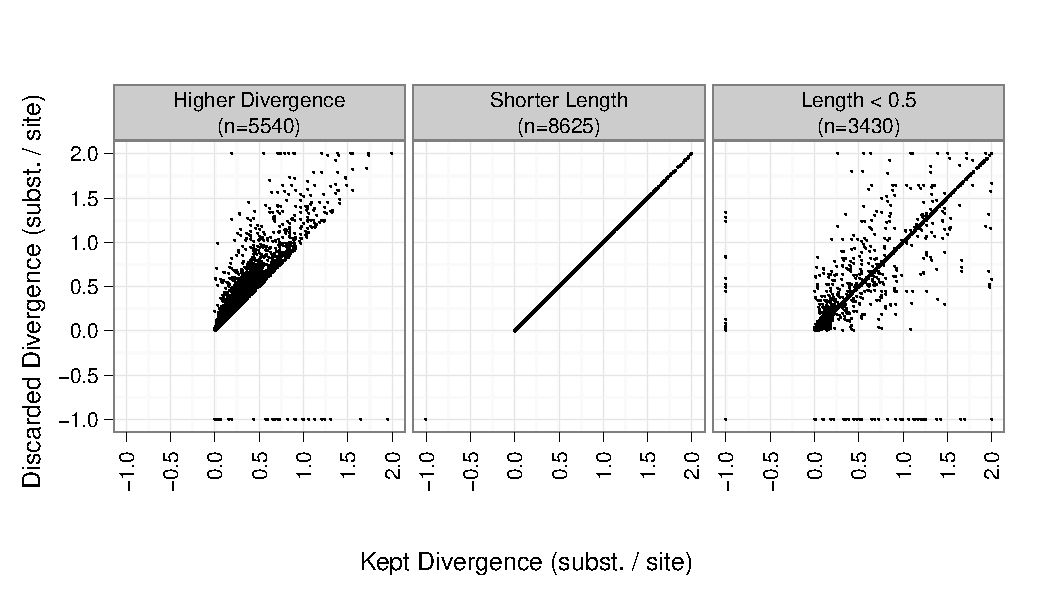
\includegraphics[scale=0.7]{Figs/filtered_paralogs_scatter.pdf}
\caption{Sequence divergence of kept and discarded putative
  paralogs. Each point represents a gene which was discarded from the
  tree for one of three reasons: it had more sequence divergence than
  the kept gene (\emph{Higher Divergence}; left panel), it had equal
  sequence divergence but shorter length than the kept gene
  (\emph{Shorter Length}; middle panel), or it had a gene length
  (relative to the mean across all sequences) of less than 0.5 while
  the kept copy had a relative length greater than 0.5 (\emph{Length
    $<$ 0.5}; right panel). Divergence was measured as the mean
  pairwise divergence between the gene and all other sequences in the
  tree, and a value of -1 was assigned to genes for which no reliable
  divergence estimate could be attained due to a lack of sufficient
  data)}
\label{filtered_paralogs_scatter}
\end{figure}

An alternate view of the results of the paralog filtering process is
shown in Figure \ref{filtered_paralogs_scatter}, with the mean
divergence of each discarded paralog compared that of the kept
paralog, separated into panels according to the reason for which the
discarded gene was removed. The spread of points above the diagonal in
the first panel shows the difference in mean sequence divergence
between the kept and discarded putative paralogs where divergence was
used to choose between copies, and the middle panel represents
paralogs whose mean divergences were identical, where length was used
as the deciding factor. These two panels together show that although
most recent paralogs within this set of gene trees contained
indistinguishable levels of sequence divergence, around 40\% showed a
moderate difference in divergences that could be used for selecting
the less-diverged copy. The rightmost panel shows the subset of
apparent paralogs which were discarded due to their short gene length;
a point worth noting here is that there was no bias towards higher or
lower divergence levels in this set of discarded genes (many of the
points lie directly on the diagonal, and the coefficient of the
best-fit linear model for all non-negative values was $0.983 \pm
0.005$), which was consistent with the prediction that many of the
discarded short genes were in fact derived from a single orthologous
gene.

\subsection{Realigning coding sequences}

After filtering out codons with low quality scores and removing
paralogs, sequences were aligned with \prank \citep{Loytynoja2008}
using its codon alignment model based on the empirical codon model
\citep{Kosiol2007}. The simulation experiments described in Chapters
\ref{ch_indels1} and \ref{ch_indels2} as well as numerous
previously-reported empirical and simulation-based studies have shown
\prank{}'s codon-based alignments to be superior for avoiding false
positives in the detection of sitewise positive selection, strongly
supporting the choice of \prank for this analysis.

\subsection{Filtering out clusters of \nsyn substitutions}

Manual analysis of a number of genes showed that even after 

A final filtering step was applied in order to ensure that stretches
of aligned but nonhomologous sequence, resulting either from
misalignment or from exon mis-annotation artifacts, were not causing
elevated rates of \nsyn substitutions within specific regions of
genes. This filtering step motivated by an observation that errors
resulting from either misalignment or exon mis-annotation would in
both cases lead to clustered regions of nonhomologous aligned
nucleotides and, correspondingly, clustered regions of elevated \nsyn
substitution rates. This clustering was expected because for both
misalignment and mis-annotation, the existence of one misaligned
column is not independent of nearby columns: for mis-annotation the
misalignment would span the entire length of the erroneously-annotated
exon, while the global nature of the progressive pairwise alignments
created by \prank{} (along with most other progressive alignment
programs) would cause any misalignment error to be tightly associated
with misalignment errors in nearby alignment columns.

These arguments suggested the possibility that clustered \nsyn
substitutions might be used as a signal to detect misaligned and
mis-annotated regions, but the utility of such a signal for filtering
alignments would also depend on the strength of error-caused \nsyn
clusters relative to the frequency of true \nsyn substitutions along a
given branch in the gene tree and to the tendency of those
substitutions to cluster together along the length of the protein
sequence. Clearly, sequences sequences separated by longer branch
lengths will show higher numbers of non-erroneous \nsyn substitutions,
possibly exceeding the number typically produced by alignment or
assembly errors, thus and reducing the ability to use substitution
clusters as a discriminating factor. Furthermore, \nsyn substitutions
have been shown to be significantly more clustered than expected by
chance in a number of genomic analyses of mammals and insects
\citep{Callahan2011,Bazykin2004,Wang2007}, causing some concern that a
filter based on detecting clusters of \nsyn substitutions might
attenuate the signal of true adaptive substitution that was one target
of the present study.



\draft{Write up the empirical investigation of \nsyn substitution clustering.}

\section{Genome-wide analysis of sitewise selective pressures in mammals}

\subsection{Mammalian species subsets for sitewise analysis}

The SLR method was applied sequentially to several species subsets of
each alignment of mammalian orthologs. For each subset, sequences
corresponding to species within the subset were extracted from the
alignment along with the corresponding \subtr and input to SLR. If
fewer than two sequences were available for a given subset, that
subset was skipped and its absence from the dataset was
recorded. Eight subsets in total were selected for analysis; the
species included in each subset and some phylogenetic measures of each
subset are listed in Table \ref{species_set_summary}.

Three subsets (Glires, Primates, and Laurasiatheria) were chosen
because they represent the three mammalian superorders with the
greatest taxonomic representation in Ensembl, providing an opportunity
to compare the molecular evolutionary dynamics of three monophyletic
mammalian groups containing varying levels of divergence, diverse
biological characteristics, and a number of high-quality reference
genomes. A fourth parallel mammalian subclade, named Atlantogenata and
consisting of sloth, armadillo, tenrec, elephant and hyrax, was also
included, but the monophyly of this group is still debated
\citep{Murphy2007,Churakov2009} and it contains only one high-coverage
genome. As such, it was not considered a primary target for the
mammalian superorder analysis.

Two larger species sets, Eutheria and Mammalia, were chosen for the
purpose of measuring average sitewise selective pressures with high
precision across a wider group of mammals. Using the Ensembl species
tree as a guide, the estimated total synonymous branch lengths spanned
by Ensembl species within Eutheria and Mammalia were 4.95 and 6.18,
respectively. Simulations performed by Anisimova and Yang
\citeyearpar{todo, Anisimova Yang 2002} and by myself in Chapter
\ref{ch_indels1} predicted that the greater amount of branch length in the
Eutherian and Mammalian trees---with two to three times the value of
1.71 for Laurasiatheria, the superorder with the largest total branch
length---would result in significantly higher levels of power and
accuracy for estimating sitewise \omg and detecting sitewise positive
selection. In this respect, Mammalia and Eutheria were more similar to
each other than to any of the superorders.

However, the Mammalia and Eutheria subsets differed markedly in a
different (and largely orthogonal) phylogenetic factor, the
evolutionary depths of their last common ancestors. Whereas the
ancestor of all Eutherian mammals lived ca. \draft{125} mya, the
Mammalian ancestor dates back to \draft{320} mya. This suggested that a
comparison between the sitewise results for the two groups might
provide useful insight into the general effect of adding longer,
deeper branches to a sitewise evolutionary analysis as well as some
indirect evidence on the molecular evolutionary dynamics of our most
distant mammalian relatives (the Eutheria and Mammalia groups only
differ by the inclusion of wallaby, opossum and platypus in the
Mammalia group).

Quantitatively, as measured by the \mpl from the Ensembl species tree,
the Eutheria subset (\mpl=0.24) is far more similar to either of the
three superorders (\mpl from 0.13 to 0.27) than to the Mammalia subset
(\mpl=0.54). This is due to the striking adaptive radiation of
Eutherian mammals \citep{Archibald1999,BinindaEmonds2007}, which
caused a quick succession of speciation events around the K-T boundary
and gives a largely star-like structure to the eutherian evolutionary
tree. Interestingly, according to the time-resolved mammalian tree
from Bininda-Edmonds et al. \citeyearpar{BinindaEmonds2007} the
Diprodontia order (containing wallaby and opossum, two outgroups to
the Eutheria clade) experienced a radiation similar to, but less
prounced than, the Eutherian radiation; a comparison of the evolution
of the deeply-rooted Diprodontia clade to its sister Eutherian clade
would be very enlightening, but the species representation of
Diprodontia (currently at one high-coverage and one low-coverage
genome) is too limited to allow for a powerful analysis. Nevertheless,
the inclusion of the three non-Eutherian species in the Mammalian
species group was expected to provide an additional data point for
aiding in an understanding of the complex relationship between branch
length, power and biological variability in the analysis of sitewise
selective pressures.

Finally, to further investigate the combined impact of evolutionary
depth, biological variability and branch length on the results of
large-scale sitewise analyses, two ``sparse'' subsets were created to
act as controls relative to two existing species subsets. The species
in the Sparse Glires group were chosen to approximate the total branch
length of the Primate clade with species from the Glires clade, while
the Sparse Mammals subset was constructed by selecting one species
(preferably with a high-coverage genome) from each major mammalian
branch, greatly reducing the total branch length covered but
maintaining a similar evolutionary depth and distribution of branches
within the species tree. The branch lengths in Table
\ref{species_set_summary} show that the Sparse Glires group was only
somewhat successful in its goal of approximating the Primates branch
length (with total branch lengths of 0.99 and 0.68, respectively)
while the Sparse Mammals group achieved a threefold lower total branch
length compared to the full Mammalia group while maintaining a nearly
identical \mpl.

% latex table generated in R 2.13.0 by xtable 1.5-6 package
% Thu Sep 15 11:19:59 2011
\begin{table}
\centering \footnotesize
\begin{tabular}{lb{6cm}rrrrr}
\toprule
 & &  & \multicolumn{2}{c}{Ensembl} & \multicolumn{2}{c}{Gene Median} \\
\cmidrule(r){4-5} \cmidrule(r){6-7}
Name & (Species Count) Species List & \Ne & MPL & Total & MPL & Total \\
  \midrule
\input{Tables/species_set_summary.txt}
\bottomrule
\end{tabular}
\caption{Species subsets used for sitewise analysis. Values under the
  ``Ensembl'' heading were calculated from subsets of the species tree
  used for evolutionary analyses by the Ensembl Compara pipeline,
  while values under the ``Gene Median'' heading were calculated as
  median values across the \ngenes gene trees analyzed (with branch
  lengths optimized by SLR). MPL -- mean path length, Total -- total
  branch length.}
\label{species_set_summary}
\end{table}

\subsection{Evaluation of the bulk distributions and the design of a filtering appraoch}

Sitewise data were collected from SLR and stored in a database for
storage and further analysis. The Mammalia subset, containing the most
branch length of all the datasets and representing the entire set of
aligned sequences, and the Primate subset, containing the lowest
overall branch length, were used to perform quality-control checks on
the sitewise data. The point of these checks were to evaluate whether
any additional filtering of the sitewise results was necessary before
characterizing the global distribution of constraint in this and the
other species subsets. Even if the sequence and alignment filters
described above were successful at reducing the number of false
positives due to incorrect input alignments, the behavior of SLR when
applied to large datasets of heterogeneous alignments has not been
well-studied, and a number of biases might have influenced the
results. A particular point of concern was that columns with different
patterns of gap and non-gap sequences, especially those with few
non-gap sequences, might yield different performance
characteristics. Although the SLR method was sensibly designed to
account for uncertainty in the estimation of \omg and detection of
positive selection, one might reasonably expect less-desirable
statistical properties from sites with 2 non-gap sequences compared to
sites with 20.

\begin{landscape}
\begin{figure}
\centering
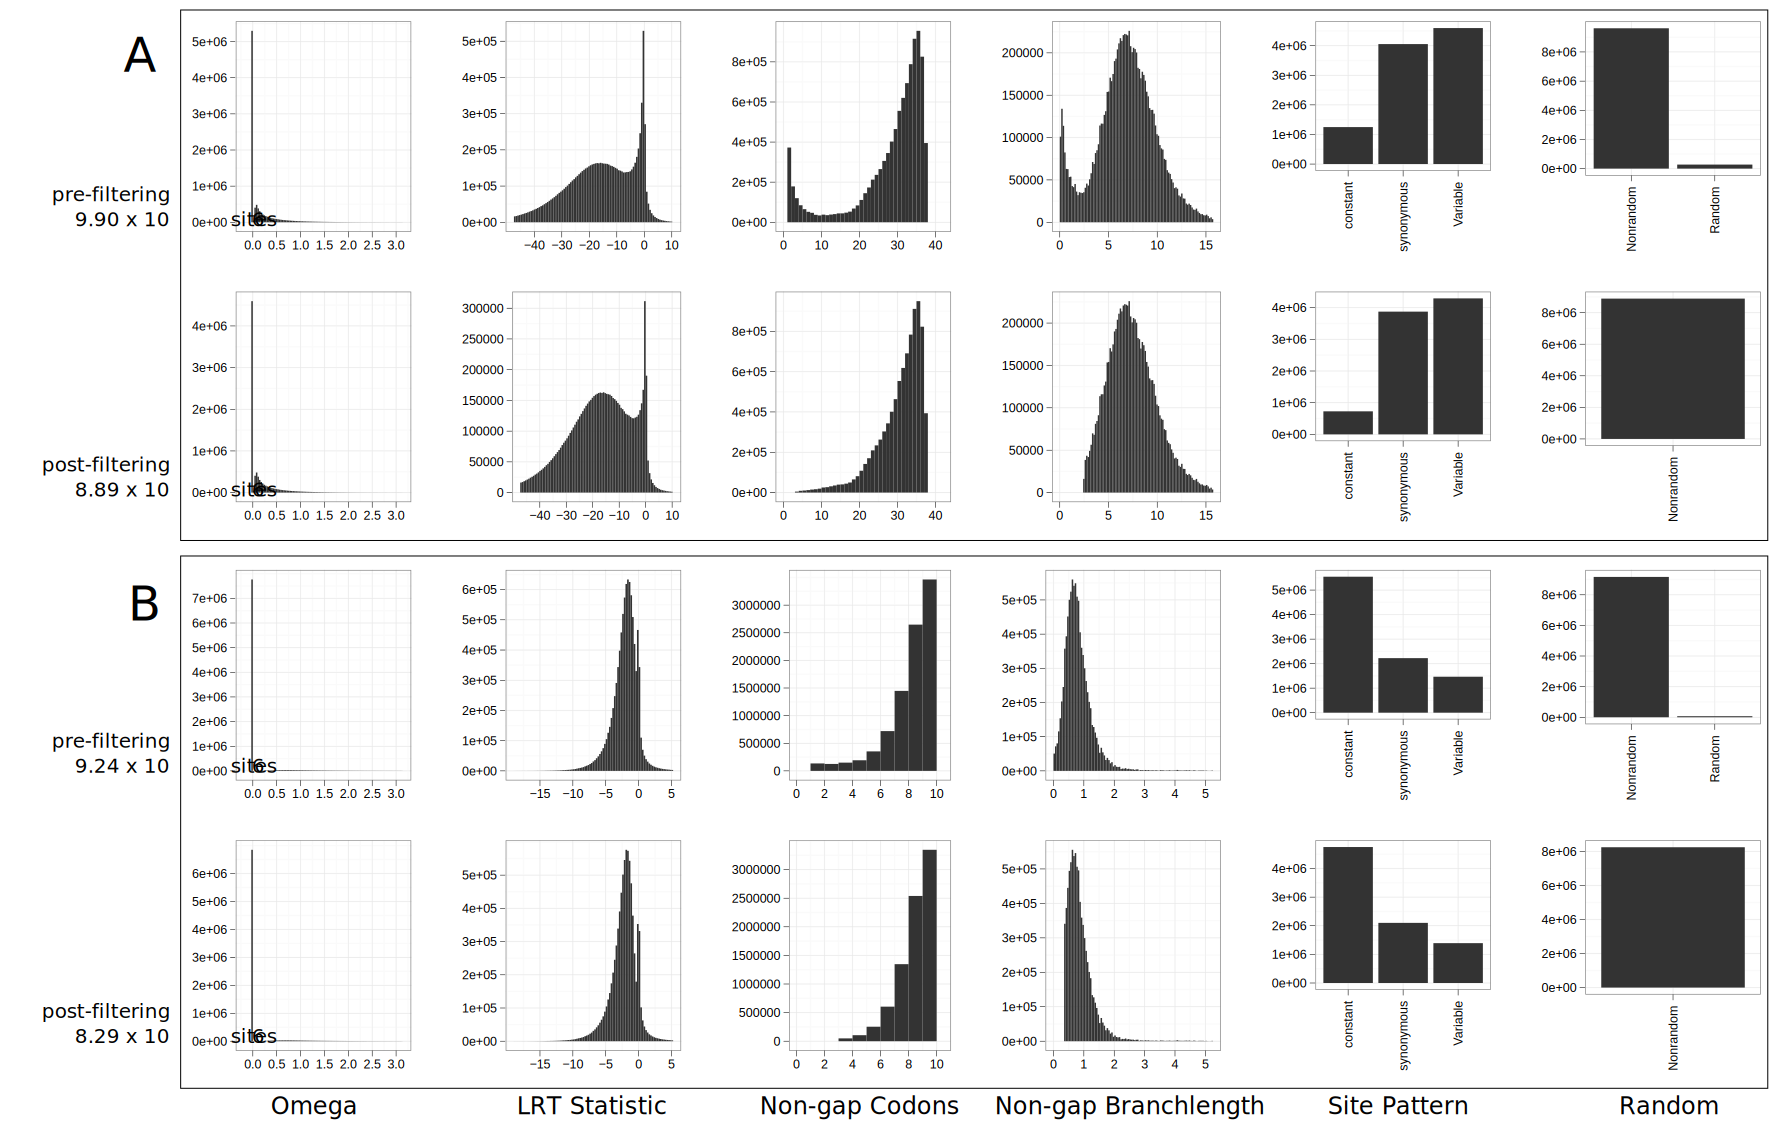
\includegraphics[scale=0.42]{Figs/qc_hist_mammals_primates.pdf}
\caption{Distributions of sitewise values for Mammalia (A) and (B)
  Primates, before (top row) and after (bottom row) removing sites
  based on the filtering scheme (see text). Note: the y-axis scale
  varies between rows, and the x-axis scale varies between (A) and (B)
  for the Signed LRT, Nongap Codons and Nongap Branch Length values.}
\label{qc_hist_mammals_primates}
\end{figure}
\end{landscape}
 
Figure \ref{qc_hist_mammals_primates} shows the distributions of six
sitewise values: two continuous values output by SLR (Omega and Signed
LRT), two categorical values from SLR (Site Pattern and Random), and
two values calculated from the codon alignment (Nongap Codons and
Nongap Branch Length). The Nongap Codons value measures the number of
non-gap codons in the given alignment columnn, while the Nongap
Branch Length represents the total branch length connecting all non-gap
sequences (using the gene tree with branch lengths optimized by SLR).

A prominent feature of the distribution of \omg values for the
unfiltered Mammalian data, shown in the top panel of Figure
\ref{qc_hist_mammals_primates}A, was the large number of sites with a
maximum-likelihood estimated \omg of zero. Further inspection of the
data revealed that all zero-\omg sites contained either \syn or
constant site patterns, and all sites with constant patterns (and
nearly all sites with \syn patterns) yielded a \ml \omg estimate of
zero. An estimate of zero for \syn sites is intuitively appropriate,
as the lack of any \nsyn substitutions throughout the tree would seem
to provide no evidence for a \nsyn substitution rate of greater than
zero. For constant sites the case is less clear, because no data
regarding the rate of either \syn or \nsyn substitutions
exists. However, given SLR's assumption of a constant \syn
substitution rate throughout each gene \citep{Massingham2005},
the \omg value which maximizes the likelihood of observing zero
substitutions is zero, since that value minimizes the \nsyn (and
total) substitution rate.

It is interesting to note that a small proportion (ca. 0.2\%) of \syn
sites resulted in \ml estimates greater than zero. Manual
investigation of a number of these sites \draft{Use the sites data and
  'seq' table to do a more quantitative analysis here?}  showed them
all to include synonymous codons with multiple nucleotide differences
(such as those coding for serine and arginine), for which SLR's
mechanistic codon model---which does not allow for multiple
simultaneous nucleotide changes--required the inference of multiple
\nsyn substitutions and, thus, a \nsyn substitution rate of greater
than zero. The existence of multiply-substituted codons in alignments
has been previously reported \citep{Averof2000,Whelan2004}, and
empirical results have supported the notion that codon models that
allow for multiple simultaneous nucleotide changes better describe
evolution than those that do not \citep{Kosiol2007}. However, the very
low proportion of synonymous sites requiring nonzero \nsyn
substitution rates suggested that the impact of these effects on the
current dataset was minimal; this is likely due to the relatively
short branch lengths separating the nodes of the mammalian tree,
making it less likely that codons with multiple substitutions (whether
the result of simultaneous multiple nucleotide changes or successive
single changes) would be observed \citep{Kosiol2007}.

The distributions of Nongap Codons and Nongap Branch Length values in
the top row of Figure \ref{qc_hist_mammals_primates}A showed that many
alignment columns contained only a few non-gap sequences. Both
distributions were bimodal with a larger peak at the upper end of the
range and a smaller peak at the lower end of the range. If the sites
with low non-gap codon counts represented accurate evolutionary
histories, the observed excess of mostly gapped sites might be taken
as an indication that insertion events in terminal lineages or recent
ancestral lineages were prominent enough in mammalian evolution to
leave a noticeable signature of sites with low non-gap codon
counts. This would be a very interesting observation, but
unfortunately it is not likely a correct one. Given the many possible
sources of error in the creation of Ensembl gene trees, however, a
more likely scenario was that sites with low codon counts and low
branch lengths came from stretches of sequence which only exist in a
few species as a result of annotation or alignment error, with a
higher probability of being nonhomologous and showing spurious signals
of positive selection. This would make such sites prime candidates for
filtering out prior to a large-scale analysis.

To test the hypothesis that sites with few non-gap sequences are less
reliable than other sites, the Mammals and Primates data were split
into deciles by nongap branch length and sites within each decile were
summarized by the proportion of sites showing evidence for purifying
and positive selection; the results of this analysis are presented in
Table \ref{bl_pos_sel_breakdown}. The lowest decile appeared to be a
clear outlier in the Mammalia dataset, with nearly 17\% of sites
having an estimated \omg of greater than 1 and 2\% of sites showing
significant evidence for positive selection at a nominal 5\% error
rate. Deciles with greater nongap branch lengths showed lower
proportions of sites with \omg $> 1$ and less evidence for positive
selection, with a gradual increase in both values at progressively
higher deciles. The gradual increase in evidence for positive
selection with increasing nongap branch length could be explained by
genes with higher overall \dnds ratios (and perhaps more positive
selection) producing, on average, higher estimated branch lengths due
to the increased \nsyn substitution rate. Overall, these patterns were
consistent with the expectation that sites with few non-gap sequences
were not consistent with the bulk of the dataset, and Table
\ref{bl_pos_sel_breakdown} showed that removing sites with the lowest
10\% of nongap branch length would remove most of the apparently
anomalous sites.

The breakdown of Primates data in Table \ref{bl_pos_sel_breakdown}
showed a trend similar the Mammalia dataset, although the distinction
between the lowest decile and the rest of the dataset was less
clear. The \fpos in the lowest decile was only slightly higher than in
the next-highest decile, and \fblw was lower than in all other
bins. The gradual increase of \fabv and \fpos in higher branch length
deciles was similar to that seen in the Mammalia dataset,
however. Despite weaker evidence in the Primates data for the
erroneous nature of sites with few non-gap sequences, it still
appeared that filtering sites in the bottom decile would improve the
overall quality and consistency of the data.

\begin{table}
\centering \footnotesize
\begin{tabular}{lrrrrrrrrrr}
\toprule
 & BL & \multicolumn{3}{c}{Nongap BL} & \multicolumn{3}{c}{Nongap Codons} & \multicolumn{2}{c}{\omgml, \%} &  \\
\cmidrule(r){3-5} \cmidrule(r){6-8} \cmidrule(r){9-10}
 & Quantile & 25\% & 50\% & 75\% & 25ff\% & 50\% & 75\% & $< 1$ & $> 1$ & \psfive, \% \\
  \midrule
\input{Tables/bl_pos_sel_breakdown.txt}
\bottomrule
\end{tabular}
\caption{Proportions of sites with evidence for purifying and positive
  selection in the Mammalia and Primates datasets broken down by
  nongap branch length. Sites were separated into 10 equally-sized
  bins of nongap branch length and summarized by the $25^{th}$,
  $50^{th}$ and $75^{th}$ percentiles of nongap branch length and
  nongap codons, the percentage of sites with \omg estimated below or
  above 1, and the percentage of sites with significant evidence of
  positive selection at a nominal 5\% FPR.}
\label{bl_pos_sel_breakdown}
\end{table}

Turning back to the bulk distributions in Figure
\ref{qc_hist_mammals_primates}, the rightmost panel depicts the small
set of sites designated as ``random'' by SLR. These sites were flagged
by SLR as having a site pattern not significantly different from
random \citep{Massingham2005}, and they were also targeted for
removal before analysis of the global distribution.

The final filtering protocol applied to each sitewise dataset included
three steps. First, all sites within the bottom 10\% of nongap branch
length values were removed; second, sites flagged by SLR as ``random''
were removed; third, all sites with fewer than four non-gap sequences
were removed.

The most prominent effect of the filter on the bulk distributions in
Figures \ref{qc_hist_mammals_primates}A and
\ref{qc_hist_mammals_primates}B was, as expected, the removal of the
excess of sites with low non-gap branch lengths and non-gap codon
counts. The distribution of \omg estimates and Signed LRT statistics
were largely unchanged, indicating that the overall characteristics of
each dataset were not significantly altered by the filter. The lack of
large-scale change was a somewhat reassuring result, given that the
filter only removed roughly 10\% of sites from each dataset.

A more detailed comparison of various summary statistics for the
filtered and unfiltered datasets showed that filtering had a
noticeable impact on three quantities of interest: it reduced the
proportion of constant sites, lowered the mean \omg, and slightly
decreased the percentage of positively-selected sites. Tables
\ref{sitewise_summary_table_1} and \ref{sitewise_summary_table_2}
contain summary statistics and calculations performed on the filtered
and unfiltered Mammalia and Primates data. Most of the data contained
in these tables will be more fully described in the next subsection,
but a comparison of the filtered and unfiltered rows for Primates and
Mammalia provided a means by which to quantitatively assess the effect
of filtering on particular aspects of the dataset. First, the
percentage of constant sites was reduced in the post-filtering data,
moving from 60.04\% to 57.62\% in Primates and from 12.62\% to 8.17\%
in Mammalia. This was expected, as the sites removed by filtering were
enriched in constant site patterns due to their lower non-gap branch
lengths. Second, the mean \omg value was slightly reduced in Primates
(from 0.32 to 0.27) and greatly reduced in Mammalia (from 0.49 to
0.20), likely due to the removal of sites containing a small number of
nonhomologous codons which might have produced abnormally high
sitewise \ml \omg estimates. Third, the proportion of
positively-selected sites (shown for a range of significance
thresholds in Table \ref{sitewise_summary_table_2}) was moderately
reduced in both Primates (from 0.56\% to 0.53\% at \chisqlt{0.05}) and
Mammalia (from 0.72\% to 0.56\%). These three effects of filtering,
each showing a shift indicating more useful data (e.g., a lower
percentage of constant sites) or less evidence for positive selection
(e.g., lower mean \omg and proportion of positively-selected sites) in
the post-filtering datasets, together provided evidence supporting the
inclusion of such a filtering step prior to the analysis and
comparison of sitewise estimates in different species sets. Although
most quantities of interest were not noticeably changed, those that
were affected by filtering shifted to more conservative values, which
was taken to be a positive sign given the persistent concern regarding
the presence of false positives in detecting positive selection.

\begin{landscape}
\begin{table}
\footnotesize{
\centering
\begin{tabular}{lllrrrrrrrrrrrrr}
\toprule
 &  & &  \multicolumn{3}{c}{Site Pattern, \%} & Med. & 
  \multicolumn{3}{c}{Nongap BL} & \multicolumn{2}{c}{\omgml} &
\multicolumn{4}{c}{\omgml Below / Above, \%} \\
\cmidrule(r){4-6} \cmidrule(r){8-10} \cmidrule(r){11-12} \cmidrule(r){13-16}
Name & Filter & Sites & Const. & Syn. & Nsyn. & Codons & Med. & Mean & SD & Mean & SD &
$< 0.5$ & $< 1$ & $> 1$ & $> 1.5$ \\
  \midrule
\input{Tables/filter_summaries_1.txt}
\bottomrule
\end{tabular}
\caption{Summary statistics and \ml \omg estimates for sitewise data
  in eight species groups. Rows labeled ``Primates (raw)'' and
  ``Mammalia (raw)'' were computed based on unfiltered data and are
  included for reference. Columns under the ``\omgml Above / Below,
  \%'' heading measure the cumulative percentage of sites with \omgml
  below or above the indicated value. Med.---median,
  Const.---constant, Syn.---\syn, Nsyn.---\nsyn, ML---\ml.
\label{filter_summaries_1}
}

\hspace{.2in}

\centering
\begin{tabular}{llrrrrrrrrrrrrrrrrrrrrr}
\toprule
 & & \multicolumn{8}{c}{Positively Selected Sites (\%)} &
\multicolumn{3}{c}{\chisqlt{0.1}, \%} &
\multicolumn{3}{c}{\chisqlt{0.05}, \%} \\
\cmidrule(r){3-10} \cmidrule(r){7-10} \cmidrule(r){11-13} \cmidrule(r){14-16}
Name & Filter & 
  \multicolumn{2}{c}{\chisqlt{0.1}} & \multicolumn{2}{c}{\chisqlt{0.05}} &
  \multicolumn{2}{c}{\chisqlt{0.01}}& \multicolumn{2}{c}{\bhfdr{0.05}} &
  Neg. & Neut. & Pos. & Neg. & Neut. & Pos. \\
%\cmidrule(r){2-3} \cmidrule(r){4-5} \cmidrule(r){6-7} \cmidrule(r){8-9}
\midrule
\input{Tables/filter_summaries_2.txt}
\bottomrule
\end{tabular}
\caption{Proportions of sites subject to positive, purifying and
  neutral selection at various \slrt thresholds. The
  Benjamini-Hochberg method \citep{Benjamini1995} was used to identify the
  \slrt threshold at which FDR$<$0.05. For columns under the headings
  ``\chisqlt{0.1}, \%'' and ``\chisqlt{0.05}, \%'', Pos. and Neg. are
  the percentage of sites with significant evidence for positive and
  negative selection, respectively, and Neut. is the percentage of
  ``neutral'' sites not showing significant evidence for non-neutral
  selection.}
\label{sitewise_summary_table_2}
}
\end{table}
\end{landscape}


\begin{landscape}
\begin{table}
\footnotesize{
\centering
\begin{tabular}{lllrrrrrrrrrrrrr}
\toprule
 &  & &  \multicolumn{3}{c}{Site Pattern, \%} & Med. & 
  \multicolumn{3}{c}{Nongap BL} & \multicolumn{2}{c}{\omgml} &
\multicolumn{4}{c}{\omgml Below / Above, \%} \\
\cmidrule(r){4-6} \cmidrule(r){8-10} \cmidrule(r){11-12} \cmidrule(r){13-16}
Name & Filter & Sites & Const. & Syn. & Nsyn. & Codons & Med. & Mean & SD & Mean & SD &
$< 0.5$ & $< 1$ & $> 1$ & $> 1.5$ \\
  \midrule
\input{Tables/pset_summaries_1.txt}
\bottomrule
\end{tabular}
\caption{Summary statistics and \ml \omg estimates for sitewise data
  in eight species groups. Rows labeled ``Primates (raw)'' and
  ``Mammalia (raw)'' were computed based on unfiltered data and are
  included for reference. Columns under the ``\omgml Above / Below,
  \%'' heading measure the cumulative percentage of sites with \omgml
  below or above the indicated value. Med.---median,
  Const.---constant, Syn.---\syn, Nsyn.---\nsyn, ML---\ml.
\label{filter_summaries_1}
}

\hspace{.2in}

\centering
\begin{tabular}{llrrrrrrrrrrrrrrrrrrrrr}
\toprule
 & & \multicolumn{8}{c}{Positively Selected Sites (\%)} &
\multicolumn{3}{c}{\chisqlt{0.1}, \%} &
\multicolumn{3}{c}{\chisqlt{0.05}, \%} \\
\cmidrule(r){3-10} \cmidrule(r){7-10} \cmidrule(r){11-13} \cmidrule(r){14-16}
Name & Filter & 
  \multicolumn{2}{c}{\chisqlt{0.1}} & \multicolumn{2}{c}{\chisqlt{0.05}} &
  \multicolumn{2}{c}{\chisqlt{0.01}}& \multicolumn{2}{c}{\bhfdr{0.05}} &
  Neg. & Neut. & Pos. & Neg. & Neut. & Pos. \\
%\cmidrule(r){2-3} \cmidrule(r){4-5} \cmidrule(r){6-7} \cmidrule(r){8-9}
\midrule
\input{Tables/pset_summaries_2.txt}
\bottomrule
\end{tabular}
\caption{Proportions of sites subject to positive, purifying and
  neutral selection at various \slrt thresholds. The
  Benjamini-Hochberg method \citep{Benjamini1995} was used to identify the
  \slrt threshold at which FDR$<$0.05. For columns under the headings
  ``\chisqlt{0.1}, \%'' and ``\chisqlt{0.05}, \%'', Pos. and Neg. are
  the percentage of sites with significant evidence for positive and
  negative selection, respectively, and Neut. is the percentage of
  ``neutral'' sites not showing significant evidence for non-neutral
  selection.}
\label{sitewise_summary_table_2}
}
\end{table}

\end{landscape}


\subsection{The global distribution of sitewise selective pressures in mammals}

\begin{figure}
\centering 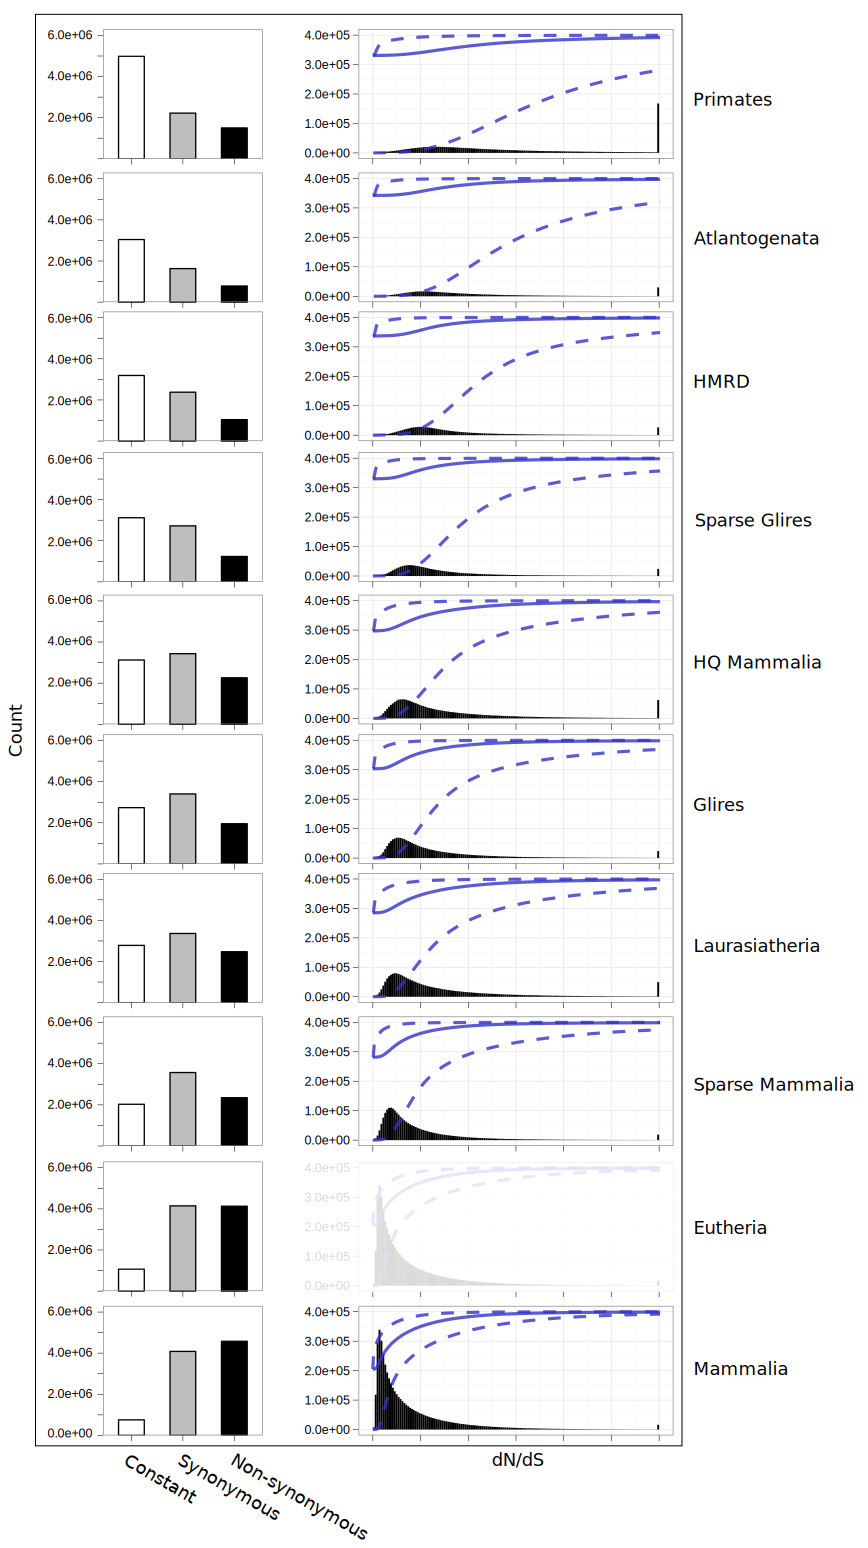
\includegraphics[scale=0.55]{Figs/global_distributions.pdf}
\caption{\scriptsize Global distributions of site patterns and \omg estimates for
  eight species groups. Left, bars represent the number of sites
  showing constant, synonymous, and non-synonymous patterns. Note, the
  y-axis is held constant between rows. Right, bars represent a
  histogram of \ml \omg estimates where $\omega>0$. Sites where
  $\omega>3$ are counted in the bin at $\omega=3$. A solid line is
  drawn showing the cumulative proportion of sites with \omg below the
  current value, and dashed lines are drawn above and below the solid
  line, showing the cumulative proportion of sites with the lower or
  upper range, respectively, of their 95\% confidence interval below
  the current value.}
\label{global_distributions}
\end{figure}

Each set of sitewise data was filtered as described above. The
resulting global distributions of site patterns, sitewise \omg
estimates, and 95\% confidence intervals are shown in Figure
\ref{global_distributions}; the left panel in each row plots the
number of sites with constant, \syn, and \nsyn patterns. All sites
with \omgml$=0$ had constant or \syn patterns, and all sites with
\omgml$>0$ had \nsyn patterns; the distributions of \omgml for these
\nsyn sites are shown as histograms on the right panel in each row.

\subsubsection{Site patterns and \omgml values reveal the prevalence of purifying selection in mammalian proteins}

The site pattern counts in Figure \ref{global_distributions} showed
that the branch length of each species group had a strong effect on
the overall composition of the sitewise data. Species groups covering
little branch length, such as Primates and Atlantogenata, contained a
majority of constant sites, while groups comprising lots of branch
length, such as Eutheria and Mammalia, contained few constant sites
and roughly equal proportions of \syn and \nsyn sites. Comparing the
Glires and Mammalia data with their corresponding ``sparse'' datasets
confirmed that this trend was largely due to branch length as opposed
to biological factors: the Sparse Glires data yielded a smaller
proportion of \nsyn sites and a greater proportion of constant sites
than the Glires data (17.41\% versus 24.08\% for \nsyn sites, 44.21\%
versus 33.98\% for constant sites; numbers from Table
\ref{sitewise_summary_table_1}), and the pattern for Sparse Mammalia
and Mammalia was qualitatively the same.

%I will cover the topic of branch length effects more thoroughly in the
%simulation study presented in Section \ref{poisson_sims}, but it
%should suffice to note here that the branch length covered by a given
%species group had a strong impact on the distribution of site patterns
%and the proportion of sites with \nsyn substitutions from which \nz
%\omg estimates could be made.

Turning to the distribution of these \omgml estimates, shown in Figure
\ref{global_distributions} as a series of histograms representing the
\omgml density (for \nz values only) and a series of solid lines
representing the cumulative density (for all values), it is clear
that the vast majority of protein-coding sites have evolved under
purifying selection in mammals. The Mammalia group, which contained a
very small proportion of potentially uninformative constant sites
(8.17\%), showed a maximum density of \nz \omgml estimates at
$\omega\approx0.1$, and the vast majority of sites showed some
evidence of purifying selection, with \omgml estimates below 1. The
height of the \omgml cumulative distribution at $\omega=1$ corresponds
to the proportion of such sites; the exact value, included in Table
\ref{sitewise_summary_table_1} under the ``$< 1$'' column, is
95.74\%. The \nz \omgml values were more evenly spread in the other
species groups, with Glires showing a maximum \nz \omgml density at
around $\omega\approx0.25$ and Primates at $\omega\approx0.7$. This
upwards shift in \nz \omgml estimates relative to Mammalia was likely
due to the greater proportion of constant and \syn sites in
lower-branch length datasets: sites which were truly evolving with
$\omega>0$, but where no \nsyn or \syn substitutions were observed,
would have their \omgml estimate ``pushed'' towards zero, causing an
increase in constant sites and a concomitant upwards shift in the
distribution of the remaining \nz \omgml values.

\subsubsection{Sitewise confidence intervals and LRT statistics identify sites with significant evidence for purifying and positive selection}

An important component of SLR's output is the set of statistics
providing information about the confidence with which purifying or
positive selection was detected. These values include the lower and
upper bounds of \ci, the 95\% confidence interval for each \omgml
estimate, and the LRT statistic, which corresponds to the strength of
evidence for purifying or positive selection. Following Massingham
\citeyearpar{Massingham2005}, I used a signed version of the
LRT statistic (hereafter \slrt), formed by negating the LRT statistic
for sites where \omgml$<1$, as a way to sort sites according to their
evidence, or lack thereof, for purifying and positive selection. Thus,
sites with \slrt$<0$ showed at least some evidence for purifying
selection and sites with \slrt$>0$ showed at least some evidence for
positive selection. It should be noted that the \slrt is a measure of
the strength of evidence for purifying or positive selection, but not
necessarily the actual strength of that selection. For example, an
alignment covering a very large branch length might yield a strongly
negative \slrt for a site with \omgml only moderately below 1, because
the difference between dN and dS was highly statistically significant;
on the other hand, a strongly-purifying site in an alignment covering
less branch length might produce a much less-negative \slrt, even with
\omgml near zero.

Figure \ref{sites_scatters}A shows the empirical relationship between
\slrt, \omgml and the \ci width for sites from the Mammali
dataset. The left panel, comparing the \slrt to \nz \omgml estimates,
shows that the two values are highly correlated, with the greatest
number of low \omgml estimates occurring at sites with strongly
negative \slrt{}s. Correspondingly, the middle panel shows an even
stronger relationship between the \slrt magnitude and the \ci width,
with the tighest windows at sites with very strong evidence for
purifying selection. The rightmost panel compares the \omgml of each
site with the width of its \ci, revealing a more linear and diffuse
positive relationship between \omgml and the size of the \ci. The
equivalent plots for Primates, shown in Figure \ref{sites_scatters}B,
reveal similar patterns, but with more weight towards less-negative
\slrt values, higher \omgml, and larger \ci. These differences
highlight the impact of branch length on the amount of confidence with
which \omg can be estimated, showing that the low branch length of the
Primates clade rarely yields \omgml estimates with \ci intervals
smaller than 1, while the bulk of sites from the Mammalia dataset have
a relatively small \ci. Thus, the \omgml distribution from datasets
with low branch lengths (e.g., Figure \ref{global_distributions})
should be interpreted with caution, and any comparison between
different sites or datasets must be sensitive to the amount of
statistical confidence placed on each estimate.

\begin{figure}
\centering
\includegraphics[scale=0.6]{Figs/sites_scatters.pdf}
\caption{The relationship between \slrt, \omgml, and \ci width in (a)
  Mammalia and (b) Primates datasets. Each point represents the binned
  density of sites; no points are drawn where no density exists, while
  blue and red points are drawn at areas of low and high density,
  respectively. The left panel shows sites where \omgml$<0$, the
  middle panel shows all sites, and the right panel shows sites where
  $0<$\xspace\omgml$<1$. Note the change in x-axis scale between plots
  in (a) and (b), reflecting the paucity of sites in Primates with
  strong evidence (\slrt$<$-12) for purifying selection.}
\label{sites_scatters}
\end{figure}

The statistical information at each site could be used to identify
sites evolving under purifying or positive selection with statistical
confidence. Sites with a \ciup, the upper bound of the \ci interval,
below \omg$=1$ showed evidence of purifying selection with an expected
5\% \fpr, and sites with a \cidown above \omg$=1$ showed evidence of
positive selection with an expected 5\% \fpr. In both cases, the 5\%
\fpr was expected under SLR's null model of neutral evolution. There
was a strong relationship between \ciup and the \chisq approximation
to the \slrt distribution, whereby the set of sites with \ciup$<1$ was
exactly equivalent to the set of sites with \slrt below the negative
\chisq 95\% critical value. Similarly, the sites with \cidown$>1$ were
those with \slrt above the \chisq 95\% critical value. Because of this
equality, I will refer to \slrt values instead of \ci intervals when
discussing sites with significant evidence for purifying or positive
selection. In some cases, however, use of the full \ci will be
preferable, as the \slrt critical values only correspond to one end of
the \ci, depending on whether the site shows greater evidence for
purifying or positive selection.

Table \ref{sitewise_summary_table_2} summarizes the results from using
the \chisq approximation to the \slrt distribution to identify sites
subject to purifying selection and positive selection at various \fpr
thresholds. The left group of columns show the number and proportion
of sites with evidence for positive selection at nominal 10\%, 5\%,
and 1\% \fpr thresholds, respectively, as well as an expected 5\% FDR
calculated using the Benjamini Hochberg method for FDR control
\citep{Benjamini1995}. The two groups of columns on the right show
the result of breaking sites into three groups (positive, negative,
and neutral) based on the result of a \chisq test at a given \fpr
threshold.

The positive selection results demonstrated that between 0.2\% to 1\%
of sites could be identified as under positive selection in mammals at
nominal FPR thresholds, but different species groups yielded
strikingly different estimates of the proportion of
positively-selected sites. At a 5\% FPR threshold, Primates,
Laurasiatheria, Eutheria, and Mammalia produced roughly comparable
proportions of positively-selected sites, ranging from 0.43\% to
0.72\%. The proportions of positively-selected sites in these groups
were higher using a 10\% FPR threshold (ranging from 0.70\% to 0.97\%
of sites) and lower using a 1\% FPR threshold (ranging from 0.14\% to
0.28\%). When the FDR was controlled using the Benjamini-Hochberg
method, however, only the Eutheria and Mammalia groups yielded a
substantial number of positively-selected sites; the Primates and
Laurasiatheria data were likely limited in their power to yield
positively-selected sites after FDR control due to their lower total
branch lengths. Interestingly, the Glires, Atlantogenata, Sparse
Glires and Sparse Mammalia datasets produced much lower proportions of
positively-selected sites across all \fpr thresholds. At FDR$<$0.05,
all four groups yielded zero significant \psc{}s.

In Mammalia, the breakdown of sites into positive, negative and
neutral categories at both \fpr thresholds produced a pattern similar
to the \omgml distribution, with overwhelming purifying constraint
(83.87\% of sites at 5\% FPR), a small proportion of
neutrally-evolving sites (15.57\%), and a small fraction of
positively-selected sites (0.55\%). As expected given the use of a
fixed \slrt threshold to identify purifying sites, the fraction of
sites confidently identified as under purifying selection showed a
strong dependency on the branch length of the species set, with a much
higher power in Mammalia than in Primates (83.87\% vs. 15.97\%).

Even for the Mammalia dataset, which encapsulated roughly 7.5
synonymous substitutions per site on average, one might reasonably
expect that the power to confidently identify sites under purifying
selection, though higher than in Primates, was still less than
100\%. If this is the case, then the proportion of confidently
identified purifying sites must be an underestimate of the true
proportion of negatively-selected sites (and by symmetry, absent any
methodological bias, the same should be true for positively-selected
sites). As a result, the fractions of positively- and
negatively-selected sites in Table \ref{sitewise_summary_table_2}
should not be taken as best estimates of the actual proportions of
such sites, but more appropriately as lower bounds on those
proportions. In fact, In the next two sub-sections, I will separately consider
the issue of using the sets of sitewise estimates in different species
groups to estimate the proportion of sites subject to purifying and
positive selection in mammals.

\subsubsection{Estimating the proportion of negatively-selected sites}

For sites under purifying selection, 

In , the value of $\approx$95\% based on \omgml$<1$ (Table
\ref{sitewise_summary_table_1}) is likely closer to the true number;
despite the caveats involved in ignoring the uncertainty involved in
\omgml estimates, the 95\% number was surprisingly consistent across
different species groups and branch lengths, ranging from
$\approx$91\% in Primates to $\approx$97\% in Sparse Mammalia.

\subsubsection{Estimating the proportion of positively-selected sites}

The pattern of the prevalence of positive selection across species
groups was surprising. First, 

, showing no sign of the expected correlation with
branch length. Theory predicts, and many studies have confirmed
\citep{Anisimova2001,Anisimova2002,Massingham2005}, that the power of LRT-based tests
for non-neutral selection should increase with branch length, as the
discrimination between \nsyn and \syn substitution rates becomes more
confident with more fixed substitutions. This was certainly the case
for identifying purifying selection, but there was no obvious
correlation between higher branch lengths and higher numbers of
confidently identified \psc{}s.

\subsubsection{Correlations between branch length, effective population size and sitewise summary statistics}

% Gotta look at these guys for Ne approximations: 
% http://www.pnas.org/content/104/51/20443.full

To quantify this observation, Spearman's rank correlation coefficients
between the median branch length of each species set and each of
several summary statistics were calculated (Table
\ref{summary_correlations}). Although the number of samples was small
with only eight species groups, these correlations should be able to
provide some indication as to which aspects of the sitewise data might
be easily attributed to the effects of branch length and which aspects
suggested an alternative (e.g., biological or artefactual) cause for
the differences between species groups. The results were quite
striking: the site classifications (constant, \syn and \nsyn) and the
proportion of negatively-selected sites at \chisqlt{0.05} were
strongly correlated with branch length, while the other factors,
including mean \omgml, the proportion of sites with \omgml$<1$ and
\omgml$<0.5$, and the proportion of positively-selected sites, were
weakly correlated or largely uncorrelated with branch length.

The results in Table \ref{summary_correlations} can be interpreted
in a number of ways. First, they emphasized the unambiguous
correlation between the branch length in a tree and the power to
detect sitewise purifying selection. However, they also showed that
various measures based on sitewise estimates contained variation
between species groups that was not well-explained by branch length. 

\begin{table}
\centering \footnotesize
\begin{tabular}{lrrrr}
\toprule
 & \multicolumn{2}{c}{Branch Length} & \multicolumn{2}{c}{\Ne} \\
\cmidrule(r){2-3} \cmidrule(r){4-5}
Value & Rho & P-value & Rho & P-value \\
\midrule
\input{Tables/summary_correlations_touchedup.txt}
\bottomrule
\end{tabular}
\caption{Correlations between median non-gap branch length, \Ne, and
  various summary statistics of the sitewise data across eight species
  sets. The magnitude (Rho) and significance (P-value) of Spearman's
  rank correlations between variables were calculated using \Ne values
  from Table \ref{species_set_summary} and branch lengths and summary
  statistics from Tables \ref{sitewise_summary_table_1} and
  \ref{sitewise_summary_table_2}. All summary statistics except for
  mean \omgml were measured as a fraction of total sites. More highly
  significant correlations are shaded in darker blue. \Ne{} -- estimated
  effective population size, BL -- non-gap branch length, \psfive
  -- positively-selected codons at \chisqlt{0.95}.}
\label{summary_correlations}
\end{table}



\subsection{Modeling the global distribution of sitewise selective pressures}
\label{modeling_distr}


\begin{landscape}
\begin{table}
\centering \footnotesize
\begin{tabular}{llrrrrrrrrrrrrrrr}
\toprule
 &  
 & \multicolumn{2}{c}{Log-normal} 
 & \multicolumn{2}{c}{Gamma} 
 & \multicolumn{2}{c}{Exponential} 
 & \multicolumn{2}{c}{Beta} 
 & \multicolumn{2}{c}{Weibull} \\
\cmidrule(r){3-4}
\cmidrule(r){5-6}
\cmidrule(r){7-8}
\cmidrule(r){9-10}
\cmidrule(r){11-12}

Species Set & Data Type
 & \omgmean & \% $>1$
 & \omgmean & \% $>1$
 & \omgmean & \% $>1$
 & \omgmean & \% $>1$
 & \omgmean & \% $>1$
\\
  \midrule
\input{Tables/distribution_fits.txt}
\bottomrule
\end{tabular}
\caption{Mean \omg and the percentage of sites with \omg$>1$ based on
  maximum-likelihood fits of parametric distributions to sitewise
  estimates. For each species set and each one of five distribution
  types (log-normal, gamma, exponential, beta, and weibull) 100
  replicate datsets of 1 million sites were sampled with replacement
  from the genome-wide dataset and the maximum likelihood distribution
  parameters were numerically optimized (see text for
  details). Columns show, for each distribution, the median value
  across 100 replicates of mean \omg (\omgmean) and the probability
  mass with \omg$>1$, expressed as a percentage (\%$>1$). The top
  eight rows show the results based on fitting parameters to sitewise
  \omgml estimates, and the bottom eight rows show the results based
  on fitting parameters to sitewise \ci estimates. Note the greater
  consistency of \omgmean and \%$>1$ across distribution types for the
  \ci{}-based fits.}
\label{distribution_fits}
\end{table}
\end{landscape}


\begin{table}
\centering \footnotesize
\begin{tabular}{llrrrr}
\toprule
Species Set & Distribution & AIC & $d$AIC & Parameter A & Parameter B
\\
  \midrule
\input{Tables/distribution_params.txt}
\bottomrule
\end{tabular}
\caption{ \scriptsize AIC values and parameters for maximum-likelihood fits of
  parametric distributions to sitewise \ci estimates. Distributions
  were fit to 100 replicate datasets for each species set as in Table
  \ref{distribution_fits}. For each species set and distribution type,
  the median Akaike information criterion (AIC) and parameter
  estimates are shown. Distributions are sorted according to their
  median AIC value (where a lower AIC corresponds to a better fit to
  the data), and the difference in AIC to the next-best fitting
  distribution is displayed ($d$AIC). The lognormal and beta
  distributions are ranked first or second in the mammalian superorder
  subgroups, while lognormal, weibull and gamma distributions fit the
  Eutheria and Mammalia datasets best. The named parameters
  corresponding to parameters A and B for each distribution are as
  follows: lognormal (A=meanlog, B=sdlog), weibull (A=shape, B=scale),
  gamma (A=shape, B=rate [where rate=$1/$scale]), beta (A=shape1
  [$\alpha$], B=shape2 [$\beta$]), exponential (A=rate [$\lambda$]).}
\label{distribution_params}
\end{table}

\begin{figure}
\centering
\includegraphics[scale=0.85]{Figs/distribution_fit_plots.pdf}
\caption{The mean value (A, Mean Omega) and the percentage of probability
  density with \omg$>1$ (B, Omega$>1$) from \ml fits of parametric distributions to
  sitewise \ci estimates. Each point represents the \ml fit of one
  distribution to 1 million points sampled from the genome-wide
  dataset with replacement; 100 such fits were generated for each
  distribution and species set. Note that the beta distribution is
  only defined on the interval (0,1), so the percentage of sites with
  \omg$>1$ was always zero.}
\label{distribution_fit_plots}
\end{figure}


% From 2xmammals supp. materials.
% https://docs.google.com/leaf?id=0B5HhSYGuKPKpYTY1YzVjNTgtODc2Yy00NzQ0LTgwZTQtMTQ3ZTA5ZWJjZGJm&hl=en_US
We used the ‘fitdistr’ function of the MASS package for R to fit five
distributions (gamma, lognormal, beta, Weibull, and exponential) to
the vertebrate dN/dS values and subsequently calculated Akaike’s
Information Criterion(AIC) for each fit. For all optimizations, a
constant value of 0.001 was added to sites where dN/dS = 0 in order to
satisfy the optimizer’s requirement that the probability functions
have a defined value for all input data. Similarly, sites with dN/dS ≥
1 were excluded from the analysis for the beta optimization. All
distributions were also separately fit to the subset of sites with
dN/dS ≥ 1; the AIC values from these optimizations were used to
compare the fit of the beta distribution to the others.

The fitdistr produced the following optimized parameters for each
function: gamma (shape=0.271, rate=1.203), lognormal (meanlog=-4.079,
sdlog=2.863), beta (shape1=0.257, shape2=1.431), Weibull
(shape=0.3882, scale=0.07151) exponential (rate=4.441). The beta
distribution yielded the lowest AIC when compared to the fit of other
distributions to the subset of sites where dN/dS ≤ 1 (-2.33e7 versus
the next best equivalent AIC of -2.11e7 for the lognormal). Of the
distributions which were fit to the whole dataset, the lognormal
distribution yielded the lowest AIC (-2.11e7), followed by gamma
(-2.03e7) and exponential (-6.45e6).

%\subsection{Analysis of sitewise estimates from the mammalian superorders}

\subsection{Simulations to evaluate the fit of empirical data to a simulated poisson process at varying branch lengths and \omg ratios}
\label{poisson_sims}

The large difference in branch lengths covered by the species sets
under investigation letd to some uncertainty in whether differences in
the observed summary statistics, such as the mean \omgml or the
proportion of sites with \omgml$<1$, were due to biological
differences between species groups (i.e., differences in the efficacy
of purifying selection resulting from population size differences) or
to branch length effects. For example, two 

I performed a small simulation
study to further investigate the interactions between branch length,
effective population size, and the summary statistics presented in
Table \ref{sitewise_summary_table_1},


\subsection{Simulations to evaluate the power to detect positive selection and estimate selective pressures}

% Table: https://docs.google.com/viewer?a=v&pid=explorer&chrome=true&srcid=0B5HhSYGuKPKpN2M0YzA5ZDQtN2FiNC00N2FhLWI0MzMtYjkwZTJmMjg2YmE5&hl=en

% Text from: https://docs.google.com/document/d/1H0hBD75a2fGmJL8l0BPQQPkcmpc6jmyT3Qr8g2zUV4A/edit?authkey=CKPKivsO&hl=en_US&authkey=CKPKivsO

Previous simulations on the power and accuracy of maximum-likelihood
methods for detecting sitewise positive selection have provided strong
evidence for increased power with increased branch length and number
of taxa [Anisimova and Yang 2002 PMID:12032251, Massingham and Goldman
  2005 PMID:15654091]. Other major effects observed have been a
reduction in power when branch lengths are very short, due to the
scarcity of data in the form of observed substitutions, and a
reduction in accuracy when branches are very long and the ancestral
reconstruction procedure becomes inaccurate due to saturation of
substitutions at synonymous sites [Anisimova and Yang 2002
  PMID:12032251]. These results have provided general guidance to
empirical analyses, but the potential effects of tree shape,
divergence level, distribution of dN/dS levels, and misalignment error
make it difficult to extrapolate expected power levels or error rates
from generic simulations to specific empirical analyses and real-world
datasets. In order to estimate the power of the SLR method when
applied to the present set of species and to quantify the power gained
from the additional 20 mammalian genomes, we ran a series of
simulation experiments with parameters tuned specifically to the
analysis of mammalian gene families. Based on the prevoius studies
described above we hypothesized that the addition of 20 mammalian
genomes to the available dataset would significantly improve SLR’s
sensitivity for detecting positive selection at a reasonable error
rate, with some portion of that improvement coming from a reduction in
alignment error due to the shorter average length of branches in the
phylogenetic tree being aligned.

We used the Indelible program [Fletcher and Yang 2010 PMID:19423664]
to simulate 100 replicate codon alignments with a root sequence length
of 500 codons for each of three trees: all 29 Eutherian mammals, the 9
mammals with high-coverage genomes, and the four-species
Human-Mouse-Rat-Dog quartet used in a number of previous comparative
analyses. The dN/dS value at each simulated site was drawn from a
discretized lognormal distribution with log(mean)=-1.864 and
log(sd)=1.201 with the maximum dN/dS capped at 3. This distribution
yielded a mean dN/dS of 0.277 and 6\% of sites with dN/dS > 1, which
is consistent with our estimates from the global mammalian
distribution. We ran each set of simulations twice: once with an
insertion and deletion (indel) rate of zero, and once with an indel
rate of 0.05 indel events per substitution event. The length of each
indel event was drawn from a discretized power-law distribution with a
parameter of 1.8, a maximum insertion or deletion length of 40 codons,
and equal insertion and deletion lengths and probabilities. Each
simulated alignment was aligned using PRANK’s codon model of evolution
and analyzed with SLR. The resulting SLR score at each human sequence
position was compared to the true dN/dS at the equivalent site in the
true alignment and used to calculate the power and accuracy of the
detection of positive selection for each set of simulated
alignments. A summary of the results is provided in Supplementary
Table S17.12.

The simulation results without indels show a dramatic increase in the
ability to detect sitewise selective pressures and sitewise positive
selection in larger mammalian trees. We used ROC curves based on the
true and inferred dN/dS values to calculate a number of statistics
summarizing the performance of sitewise inference under each tree
tested. The Spearman’s rank correlation coefficient between inferred
and true dN/dS was 0.749, 0.849, and 0.942 in the 4-taxon, 9-taxon,
and 29-taxon trees, respectively, representing a 10\% increase in the
accuracy of inferred maximum-likelihood dN/dS values as a result of
the added 20 mammalian species. The number of true positives recovered
when controlling for a false discovery rate (FDR) below 0.1 was 50,
782, and 3760 for the three trees; for FDR < 0.05, the numbers of true
positives were 10, 429, and 2990. This represents a 4.8-fold increase
for FDR<0.1 and a 6.9-fold increase for FDR<0.05 resulting from the
additional 20 species in the tree. It should be noted that the two
previous power estimates re

\subsection{Evaluation of the effect of GC content, recombination rate, and codon usage on sitewise \dnds estimates and the detection of positive selection}

\begin{landscape}
\begin{table}
\footnotesize{
\centering
\begin{tabular}{rrrrrrrrrrrrrrrrrrrr}
\toprule
 & Species &  & & Med. &
 & \omgml &  & \omgml & \multicolumn{2}{c}{Recomb., cM} & & \multicolumn{3}{c}{Substitutions \%} \\
Variable & Group & Quantile & Sites & BL & \nsten
 & $<0.5$ & \psten & $>1.5$ & Male & Female & GC & Total & CpG & W-S & S-W & Nsyn \\
  \midrule
\input{Tables/recomb_quantiles_6.txt}
\bottomrule
\end{tabular}
\caption{}
\label{recomb_quantiles_mammalia}
}
\end{table}
\end{landscape}

\begin{landscape}
\begin{table}
\footnotesize{
\centering
\begin{tabular}{rrrrrrrrrrrrrrrrrrrr}
\toprule
 & Species &  & Sites & Med. & \chisqlt{0.1}
 & \omgml & \chisqlt{0.1} & \omgml & \multicolumn{2}{c}{Recombination} & & & & & & \\
 Variable & Group & Quantile & Sites & BL & Neg.
 & $<0.5$ & Pos. & $>1.5$ & Male & Female & GC & WS & CpG & Nonsyn.& Syn. & \\
  \midrule
\input{Tables/recomb_quantiles_1.txt}
\bottomrule
\end{tabular}
\caption{}
\label{recomb_quantiles_mammalia}
}
\end{table}
\end{landscape}



Multiple lines of evidence have lent support to the hypothesis that
GC-biased gene conversion (BGC) has been a major force in the
evolution of mammalian genomes [Galtier et al 2001 PMID:11693127,
  Galtier 2003 PMID:XYZ, Dreszer et al 2007 PMID:17785536]. Both
empirical and theoretical results have shown that BGC can
significantly affect patterns of observed substitutions in both
selectively neutral and functionally constrained sites [Galtier et al
  2009 PMID:19027980, Berglund et al 2009 PMID:19175294]. Recently,
Ratnakumar et al. [2010, PMID:20643747] re-analyzed the dataset of
positively-selected genes from Kosiol et al. [2008, PMID:18670650] for
signatures of BGC and found that up to 20\% of cases of identified
elevated dN/dS ratios could be due to BGC rather than adaptive
evolution. However, the strongest signals of BGC were found only in
genes showing signals of positive selection along short branches in
the phylogenetic tree using so-called branch-site models of evolution;
when the authors looked for similar BGC signatures in genes with
evidence for positive selection at specific sites throughout the
mammalian tree (e.g., genes with significant LRTs for PAML’s sites
model) they found no evidence for a strong BGC influence [Ratnakumar
  et al. 2010 PMID:20643747].

The above evidence suggests that although BGC has the potential to
produce misleading signals of branch-specific positive selection near
recombination hotspots, the positively-selected sites we detected
should not be strongly influenced by the non-adaptive effects of BGC
since the dN/dS level detected by SLR is estimated from across the
entire input phylogeny [Massingham 2005 PMID:15654091]. This is
consistent with the observation that recombination hotspots (where
most recombination in humans and other mammals occurs [Myers et
  al. 2005 PMID:16224025]) tend not to be maintained over long
evolutionary periods, although larger-scale recombination rates are
likely more conserved [Winckler et al 2005 PMID:15705809]. Still, due
to the potential confounding implications of BGC on the interpretation
of signals of positive selection, we found it worthwhile to to
empirically test for any BGC effect on our data.

The BGC model predicts a recombination-associated drive towards the
fixation of GC alleles at heterozygous sites, resulting in an expected
correlation between AT to GC (or weak-to-strong, W-S) mutational bias
and recombination rate [Galtier and Duret 2007, PMID:17418442]. This
bias can lead to elevated dN/dS estimates in coding regions,
particularly in GC-rich regions where W-S mutations are more likely to
result in nonsynonymous changes [Berglund et al 2009]. Ratnakumar and
colleagues identified three ways of distinguishing potential BGC
effects from true signals of positive selection in protein-coding
regions: (a) positive selection is not expected on its own to result
in a strong W-S bias, (b) a BGC-associated W-S biased mutation pattern
should extend to noncoding sites flanking the affected coding region,
and (c) BGC is associated with recombination hotspots and regions of
high recombination rates (and most strongly with male-specific rates)
while there is no empirical evidence linking positive selection with
higher recombination rates in mammals, although natural selection
should theoretically be more efficient in regions of high
recombination [Ratnakumar et al. 2010, PMID:20643747]. We could not
use (a) or (b) to detect possible BGC influence since we did not
calculate inferred ancestral mutations for either the coding or
flanking noncoding regions of the mammalian gene families studied
here. Instead, we turned to point (c) and tested for a correlation
between signals of positive selection and an increase in recombination
rates, especially the male-specific rate and in regions of high GC
content. The predictions of the BGC hypothesis suggest that if our
sitewise data do contain a strong BGC influence, then the
positively-selected sites we detected would be expected to be
associated with regions of high male-specific recombination.

We combined the sitewise codon data with male, female, and
sex-averaged recombination rates derived from the deCODE map (using
rates averaged over genomic bins of 1Mb downloaded from the UCSC human
genome browser hg19 release) and human GC content calcualted in 10-kb
windows and analyzed sites within various quantiles of GC content,
mean recombination rate, and sitewise statistics. Supplementary Table
S17.13 contains summaries for each subset. The ‘LRT statistic’ section
shows that sites with higher LRT statistics (which corresponds to
weaker purifying selection when the value is below zero and stronger
positive selection when the value is above zero) show decreasing
recombination rates; this trend holds true even for the highest
quantile (mean signed\_lrt between 3.648 and 108.850), which is
composed entirely of sites with evidence for positive selection. In
other words, the bulk of positively-selected sites are in regions of
lower than average male recombination rates -- exactly opposite what
would be expected in the face of strong BGC effects. The ‘Male
Recombination’ quantiles show a similar trend, with the mean dN/dS,
mean signed LRT and the proportion of sites identified as
positively-selected (pos\_f) all consistently decreasing as the
recombination rate increases. The ‘GC content’ quantiles showed a
slightly different pattern. Although the mean LRT decreased and male
recombination increased monotonically with increasing GC content, the
mean dN/dS and fraction of positive sites started low, increased to a
maximum in the middle range of GC content, and decreased again in
regions of high GC content. Thus, although the GC content quantiles
were similar to the male recombination quantiles in their higher range
(with similar mean dN/dS, mean LRT, and pos\_f values), they differed
slightly in their lower range (with lower dN/dS and pos\_f for low GC
quantiles). Although the exact reason for such a pattern is unclear,
it is consistent with the existence of altered or constrained
selective or mutational dynamics at the extreme ends of the genomic
distribution of GC content. As GC content has been shown to correlate
with myriad structural and evolutionary features of mammalian genomes
[Xia et al. 2009 PMID:19521505], the existence of other (possibly
unrelated) confounding influences such as CpG mutability or isochore
structure is likely.

Theoretical and empirical evidence pointed towards an increased
sensitivity of dN/dS estimates to BGC influence in regions of high GC
content, so we separated out the top 10\% of sites by GC content and
analyzed them according to quantiles of male recombination rate
(Supplementary Table S17.13, ‘High GC, Male Recombination’. The middle
four recombination quantiles showed a similar pattern to that observed
for all GC contents, with mean LRT decreasing with increased male
recombination and mean dN/dS and pos\_f decreasing or hovering around
values slightly lower than those observed across all GC contents
(e.g., mean dN/dS in the 1-25\% bin is 0.207 for the top 10\% GC
sites, but 0.249 for the same recombination bin across all sites). The
highest recombination bin of the top 10\% GC sites showed a strikingly
different pattern, however, with mean dN/dS=0.348, mean LRT=-11.262,
and pos\_f=0.0338. These values suggest a strong shift towards higher
dN/dS values and more positively-selected sites. This jump in values
in the highest recombination bin is not seen in the highest male
recombination bin across all GC contents (mean dN/dS=0.207, mean
LRT=-16.616, pos\_f=0.00932) or for the highest female recombination
bin for the top 10\% of GC sites (mean dN/dS=0.164, mean LRT=-18.475,
pos\_f=0.00449). Although the small number of sites in the bin of
interest compared to other bins suggests possible stochastic
artifacts, the shift is dramatic, directly opposite to the trends
observed for the female recombination rates and for male recombination
rates in regions of lower GC content, and is in agreement with the BGC
prediction of elevated dN/dS estimates in regions of high GC content
and male-specific recombination rates. This evidence raises the
interesting possibility that BGC may have a detectable, if rather
minor, impact on sitewise dN/dS estimates across the mammalian
phylogeny. It is highly unlikely, however, that any such effect --
which in our analysis was only detectable in 0.05\% of sites with the
most extreme GC content and recombination rates -- has contaminated
our codon-specific estimates with more than a negligible amount of
noise resulting from the neutral but biased process of BGC.

\section{Conclusions}

\tocite{Eory et al. 2010}{Showed, through constraint analysis of
  various sequence types, that there is higher selective constraint in
  4-fold sites in priamtes compared to murids. Quote: ``It is well
  established that in several organisms, mutations at 4-fold sites are
  selected against (Chamary et al. 2006; Rocha 2006; Drummond and
  Wilke 2008) and as a consequence the dN/ds ratio, which has been
  frequently used to detect the strength and direction of selection
  (e.g., Dorus et al. 2004; Wang et al. 2006), may be
  underestimated. Our result of higher 4-fold constraint in hominids
  suggests that this bias more strongly affects hominid estimates and
  it may well exceed 20\%.''}

\tocite{Ohta 1993, 1995; Eory et al. 2010}{The Keightley et al. 2011
  paper (ABC to estimate mutation rate parameters) cited Ohta 1993,
  1995 and Eory et al. 2010 for the effective population size and
  efficacy of selection in primates vs. murids}

\tocite{Wolf et al. 2009}{Wolf et al. GBE 2009, used pairwise dN dS
  counts to try to show that trends in dN/dS ratios are a result of
  branch length, at least when calculated in a pairwise
  fashion. Slightly unconvincing stuff... could be cited as somehow
  relating to the discussion regarding eff. pop. size, branch length,
  and selection}

\tocite{Berglund et al. 2009}{Berglund et al. 2009 looked at hotspots
  of biased substitutions in humans. Showed that exons with
  accelerated rates in humans have a tendency towards clusters of
  AT-to-GC (weak-to-strong) substitutions. Did some simulations
  showing that this effect is strongest in GC-poor regions, though the
  impact on overall dN/dS is probably minimal (e.g., genes with
  overall high dN/dS didn't show BGC, only the most accelerated exons
  did) and the effect on dN/dS is highest in high-GC regions. The
  most-accelerated exons tend to reside in high-male (but not female)
  recombination, and <50kb from hotspots. Upshot: these biased
  clusters seem to show up in isolated regions (exons), rather than
  spread throughout entire genes. Probably not a huge impact on
  overall apparent constraint.}

\tocite{Duret and Arndt PLoS Gen 2008}{Duret and Arndt 2008 use
  nonreversible nucleotide models to estimate NEUTRAL rates correlated
  with recombination, GC, and GC*. Lots of stuff here, but the
  important bits: overall mutation rate increases with increasing GC
  content (due to overall higher rates of S-W substitution);
  recombination should have a strong impact on W-S substitution, but
  weak impact on S-W substitutions; CpG deamination varies by factor
  of two, very low in GC-poor regions and very high in GC-rich ones.}

\tocite{Galtier et al. TrIG 2009}{Galtier et al. TRIG 2009 is similar
  to Berglund et al. in many ways -- find accelerated exons in a
  primate branch, and identify significantly higher male recombination
  rates there. The number of accelerated exons is small -- ~100 in
  each of four branches -- and not all of these accelerated exons
  showed strongly elevated dN/dS ratios. Only 19 exons at the 1\%
  level. However, they do some nice modeling (mostly in the
  supp. material) which shows that the effect of BCG on dN/dS ratio at
  different GC contents -- it has more effect in GC-rich genes.}

\tocite{Capra and Pollard 2011}{Capra and Pollard quantified BDS
  (biased divergent substitutions) across metazoans, additionally
  using recombination rate data. Dog has the strongest, mouse has the
  weakest BDS scores. (This could be due to lower rec. rate in mouse,
  e.g. Coop and Przeworski 2006)}

\tocite{Nordborg et al. 1996}{Nordborg et al. 1996 (Genet. Res.)
  modeled the effect of background selection on variation in neutral
  linked loci. They showed that weakly selected mutations, rather than
  strongly selected ones, are more likely to produce regional
  patterning of variation in response to local recombination
  rate. Should have a large effect in Drosophila but small effect in
  mammals, though in mammals ``local reductions in regions of reduced
  recombination might be detectable.''}

\tocite{Chun and Fay 2011}{Chun and Fay 2011 (PLoS Gen) looked at
  neutral and deleterious SNP density according to local recombination
  rate, showing that in 'hitchhiking' regions there are fewer neutral,
  but as many deleterious, polymorphisms. That stuff is boring, but
  they also show that the deleterious SNP density stays constant
  throughout the range of recombination rates, while the neutral and
  synonymous SNP density decreases. Thus, slightly deleterious
  mutations are less effectively purged in regions of low
  recombination.}

\tocite{Bullaughey et al. 2008}{Bullaughey et al. (2008, Gen. Res.)
  looked at gene-wide dN/dS ratios in primates and recombination
  rates. They found no significant correlation between broad- or
  fine-scale recomb. rates and rates of protein evolution, **once GC
  content is taken into account**.}

\tocite{SPencer et al. 2006}{Spencer et al. (2006 PLoS Gen) Quote: ``In short,
  while there is a strong relationship between recombination and GC
  content, most of the relationship is explained by scales broader
  than recombination hotspots (16 to 256 kb; unpublished data) and may
  well result from interactions of both factors with additional
  processes such as chromatin organisation or replication
  timing. Similar arguments apply to the question of whether a GC bias
  in recombination-associated mutation can explain the relationship
  between GC content and recombination.''}

\draft{...}


%************************************************
\chapter{Characterizing the evolution of genes and domains in mammals using \sw selective pressures}
\acresetall
\label{ch_mammals2}
%************************************************
\section{Introduction}

Since the first non-human mammalian genomes were sequenced, there has
been great interest in using comparative data to identify genes
showing signatures of positive selection in mammals. Much of this
interest stems from the prospect that such genes may reflect the
historical impact of natural selection acting to fix beneficial
mutations within a population over time---a major driving force in the
modern molecular interpretation of Darwin's theory of natural
selection \citep{Endo1996,Hughes1999}. Previous scans for positive
selection in primate genomes have revealed enrichments for \acp{psg}
related to sensory perception and olfaction \citep{Clark2003},
apoptosis and spermatogenesis \citep{Nielsen2005}, and iron ion
binding and keratin formation \citep{Macaque2007}; analyses in other
mammalian genomes have revealed largely similar patterns
\citep{Kosiol2008,Li2009a}. To explain the increased \dnds values
observed within \acp{psg}, three distinct evolutionary dynamics have
commonly been invoked: an evolutionary arms race between genes
involved in host--pathogen interactions
\citep{Yang2005c,Meyerson2011}, sexual selection or genetic conflict
between the sexes \citep{Wyckoff2000,Clark2000}, and functional
adaptation following gene duplication or environmental changes
\citep{Zhang2002}.

As the power of phylogenetic analysis using codon models depends
strongly on the amount of branch length encompassed by the species
being compared \citep{Anisimova2001,Anisimova2002}, there was some
reason to believe \emph{a priori} that the detection of \acp{psg}
using mammalian alignments incorporating \lcv genomes would be more
powerful than in previous whole-genome analyses, which typically
included 12 or fewer species across mammals and lower total branch
length \citep{Ellegren2008}. However, differences in the specific
models used to detect positive selection are expected to affect the
sensitivities of one study compared to another \citep{Anisimova2009},
so the set of genes identified using the current methodology would not
necessarily be expected to overlap significantly of those identified
in previous studies. Most large-scale studies have used the
branch-site test for positive selection \citep{Zhang2005}, while the
results described in this chapter were generated using \ac{slr}. I
showed in Chapter \ref{ch_indels1} that \ac{slr} has similar power to
the site-based test implemented in PAML for detecting \sw positive
selection, but no analysis has yet compared the differences in
\acp{psg} identified by site-specific and branch-site methods on a
large scale. For this reason, I hoped that a quantitative comparison
between \acp{psg} identified using the current methodology and those
found in previously-published studies may improve our understanding of
how similar or different the \acp{psg} identified by different methods
can be.

This chapter describes the use of \sw data to identify trends in the
evolution of protein-coding genes and domains, focusing on the
detection of \acp{psg}. I first develop a number of methods for using
\sw estimates to identify signals of positive selection within genes
and apply these methods to the \sw data generated in Chapter
\ref{ch_mammals1}. Next, to provide a higher-level interpretation of
these results I use \ac{go} annotations to identify categories
enriched for genes with evidence of positive selection in different
species groups. A quantitative comparison to results from the
literature is provided through a direct comparison of the \acp{psg}
and \ac{go} term results to previously-published studies. Finally, I
apply the same methods for combining \sw estimates to identify protein
domains with the strongest enrichment for positive selection
throughout mammalian evolution.

\section{Combining \sw estimates to identify positive selection}
\label{sec_combining_sites}

In Chapter \ref{ch_mammals2} I covered the generation and analysis of
several highly filtered sets of genome-wide \sw selective pressures
within different groups of mammalian species. These \sw estimates were
used to characterize the global distribution of evolutionary
constraint and to compare overall levels of purifying and positive
selection between groups of mammalian species. The focus on individual
codons as an evolutionary unit of investigation is relatively
uncommon, but it allowed for large-scale differences in evolutionary
trends between species groups to be identified and for the impact of
different filtering schemes on overall signals of positive selection
to be easily assessed.

The more traditional approach in comparative genomics has been to
model the protein-coding gene as the unit of analysis. For detecting
positive selection, the grouping of alignment sites into genes---which
results in identification of \acp{psg} instead of \acp{psc}---has
three main advantages. First, the combined analysis of many alignment
sites improves the accuracy of estimated evolutionary parameters and
boosts the power of \acp{lrt} for detecting positive selection. This
is seen in the simulations of \citet{Anisimova2001,Anisimova2002},
which showed large power differences for detecting positive selection
in alignments simulated with 100, 200, and 500 codons. Second,
detailed studies of \sw selective pressures in genes with strong
signals of positive selection have usually observed clusters of
positively-selected sites within genes \citep{Sawyer2005a,Kosiol2008},
suggesting that the evolutionary dynamics causing detectable signals
of positive selection tend to affect many functionally or structurally
related amino acid sites within genes as opposed to acting on randomly
distributed sites. The third argument in support a gene-centric
analysis of positive selection is that in the absence of a protein
structure for every gene, much more tends to be known about entire
genes (through the results of high-throughput studies and experiments
in model organisms) than is known about the function of individual
protein-coding sites. Thus, a gene-centric analysis allows a dataset
to be more easily analyzed in connection with abundant external
functional data, benefitting the biological interpretation of results.

A major issue in combining \sw estimates to identify \acp{psg} is that
of correcting for performing multiple \sw tests per gene. The \ac{slr}
method performs an independent statistical test at each site,
producing a sitewise statistic which can be compared to a \chisq
distribution to yield a \pv representing the strength of evidence
against strict neutral evolution \citep{Massingham2005}. When
combining these \pvs to decide whether a gene contains significant
evidence for positive selection, the number of tests performed must be
taken into account. For example, a 100-codon gene evolving under the
null model ($\omega=1$) would be expected to produce 5 sites with
\pvs at a nominal \ac{fpr} of 0.05; correspondingly, the chance
that at least one site within the gene would have $p<0.05$ is
99.4\%. This is calculated as the complement of the probability that
no sites out of $n$ have $p<x$, which is $(1-x)^{n}$. Thus, if the set
of genes containing at least one site with nominal $p<0.05$ were
called \acp{psg}, nearly all genes evolving under the true null model
would be selected. In contrast, the \ac{lrt}s for positive selection
implemented in PAML only perform one statistical test per gene and do
not suffer from the same multiple testing problem. Clearly, some
procedure for correcting or combining the results from multiple tests
must be applied in order to identify \acp{psg} using \sw data in a
statistically controlled manner.

I tested 3 types of methods which are capable of correcting for
multiple \sw tests within genes to identify \acp{psg}: first,
adjusting significance thresholds to control the \ac{fwer}; second,
combining \pvs from multiple tests to produce a single \pv
summarizing the overall evidence against the null hypothesis; third,
estimating empirical gene-wise \pvs based on the genome-wide
distribution of \sw estimates. Each approach makes different use of
the \sw data from each gene to identify a set of significant \acp{psg}
and thus had the potential to identify slightly different sets of
\acp{psg}. The remainder of this section provides a description of how
each of the three approaches was applied to the \sw data.

\subsection{Controlling the \ac{fwer}}

The \ac{fwer} is defined as the probability, for a given set of tests
performed, of one or more tests producing a false positive result. In
the example of a 100-codon gene evolving under the null model, the
\ac{fwer} at a nominal \pv of 0.05 was 0.994. Assuming an
appropriate uniform null distribution of \pvs and independence
between tests, the \v{S}id\`{a}k equation (to which the popular
Bonferroni correction is a more easily computed approximation)
identifies the \pv threshold $x$ which is necessary to control the
\ac{fwer} at the desired level $\alpha$. The \ac{fwer} expected for a
family of $n$ tests thresholded at a nominal \pv of $x$ is
$\alpha=1 - (1 - x)^{n}$, so the \pv threshold necessary to
control for a desired \ac{fwer} can be found by rearranging the
equation: $x=1 - (1 - \alpha)^{1/n}$. A similar but more powerful
approach to controlling the \ac{fwer} is the step-up method from
Hochberg; this method is implemented internally by \ac{slr} for
reporting the number of positively- and negatively-selected sites
after multiple testing correction \citep{Hochberg1988,Massingham2005}.

To identify \acp{psg} by controlling the \ac{fwer}, I used the
$p.adjust$ method from the R statistical project to apply the Hochberg
procedure to the set of \sw \pvs from each gene. This produced a
new set of \pvs representing the \ac{fwer} expected if all sites
with \pvs equally or more extreme than the given site were called
significant. The overall \pv for each gene was taken as the
minimum \ac{fwer}-adjusted \pv across all sites.

One expected weakness of this approach was that the evidence for a
\ac{psg} comes only from the site in each gene with the most extreme
\slrt, ignoring any signal of positive selection from sites with
weaker \pvs. As it has been previously observed that \acp{psg}
tend to contain multiple sites subject to similarly strong amounts of
positive selection \citep{Sawyer2005a,Kosiol2008}, the gene-wise
$p$-values resulting from the \ac{fwer}-controlling approach were
expected to lack some power. The next two methods described are both
sensitive to more than just the most significant site, making them
potentially more powerful for identifying \acp{psg}.

\subsection{Combining \pvs}

The second approach to multiple testing addresses the potential
weakness of the \ac{fwer}-controlling approach by combining \pvs from
all \sw tests performed, producing an overall \pv for the null
hypothesis given the overall set of tests. The motivation behind such
methods is that moderately significant results from independent tests
of a common null hypothesis should be considered as good or better
evidence than one strongly significant test. Many different techniques
of this type have been discussed in the literature (see
\citet{Cousins2007} for an extensive annotated bibliography). Two of
the most popular methods are Fisher's combined probability test and
Stouffer's method (\citealp{Fisher1932}; \citealp{Stouffer1949};
reviewed in \citealp{Whitlock2005}). Both methods first combine the
set of \pvs from independent tests in some way: Fisher's test takes
the product of all \pvs, while Stouffer's method transforms
\pvs into normal quantiles and sums the resulting z-scores. The
combined statistic is then compared to the expected null distribution
given the same number of input \pvs. A comparison of both tests by
\citet{Darlington2000} suggests that they provide similar power
overall, but that Stouffer's method generally yields smaller \pvs
when the input \pvs are more similar and Fisher's test yields
smaller \pvs when the input \pvs vary widely.

When the distribution of input \pvs is nonuniform or the number of
tests is large, however, performance of Fisher's and Stouffer's
methods can be reduced. \citet{Zaykin2002} noted that a relatively
small number of large \pvs can limit the power of Fisher's test,
and the Stouffer method can be expected to be equally sensitive to a
bias towards large \pvs. Since the majority of the \sw estimates in
mammals showed moderately strong signals of purifying selectio, the
distribution of one-sided \pvs for positive selection was heavily
weighted towards 1. This can be seen clearly in Figure \ref{fig_xyz},
which shows a histogram of genome-wide one-tailed \pvs based on the
Mammals species group. The standard versions of both Fisher's and
Stouffer's methods were expected to lack power to identify \acp{psg}
given the strong impact of purifying selection on the \sw data.

The variants of Fisher's and Stouffer's methods which incorporate a
truncation step (i.e., including only \pvs below a pre-specified
threshold to calculate the combined statistic) provided a potentially
more powerful approach to combining \sw \pvs within genes
\citep{Darlington2000,Zaykin2002,Zaykin2007}. Zaykin et
al. \citeyearpar{Zaykin2002,Zaykin2007} showed that the \ac{tpm}, a
truncated version of Fisher's product method, is well-suited for
large-scale genomics experiments where the number of tests is large
and the standard methods lack power. The authors suggest a truncation
threshold of $p<0.05$ provides a good balance of sensitivity and
power, and they note that the method is asymptotically equivalent to
Fisher's combined test as the \pv trunctation is increased to
1. Thus, the truncation threshold determines the extent to which the
method focuses on more significant test results. The test statistic is
calculated as the product of all \pvs below the truncation
threshold, and in the implementation provided by Zaykin get
al. \citeyearpar{Zaykin2002} the significance of the statistic is
determined by simulation based on the null model. As an example, for a
gene with 100 sites and 5 where $p<0.05$, the test statistic would be
the product of those 5 \pvs and its significance would be tested
by generating 5,000 replicates under the null model (i.e., uniformly
distributed \pvs) using the same $p<0.05$ criterion to calculate
the truncated product of \pvs.

To explore the behavior of the \ac{tpm} at various \pv truncation
thresholds, I used the implementation provided by Zaykin et
al. \citeyearpar{Zaykin2002} to calculate combined \pvs at
truncation thresholds corresponding to a nominal 5\%, 10\%, 20\%, and
50\% \sw \acp{fpr}. I also calculated a combined \pv using
Fisher's standard combined method to test the hypothesis that the
method lacked power to detect \acp{psg} in protein-coding genes due to
the presence of many purifying sites.

\subsection{Assigning empirical \pvs based on the global \sw distribution}

The previous two approaches are fairly generic statistical methods,
with formulas whose accuracy depends on the assumption of
uniformly-distributed \pvs under the null hypothesis. Since the
overall distribution of one-tailed \pvs from \sw estimates is far
from uniform, however, the large proportion of sites with strong
evidence for purifying selection may cause problems when a uniform
distribution of \pvs is assumed. This problem is alleviated
somewhat by the fact that \ac{fwer} control mainly uses only the most
significant test result to identify a \acp{psg}. The sensitivity of
the \ac{tpm} method to largely non-uniform \pvs should also be
reduced, as sites with \pvs above a certain threshold from the
calculation of the combined statistic, thus avoiding undue influence
from non-significant \pvs. Still, the apparent mismatch between
the neutral null model tested by \ac{slr} and the large majority of
sites evolving under purifying selection suggested that tests based on
the theoretical distribution of \ac{lrt} statistics may be overly
conservative. For the confident identification of \acp{psg} this may
be desirable, but for the global analysis of functional trends in
genes subject to \acp{psg}, a less conservative approach should
provide more signal. Given the large set of \sw estimates available
for each species group, the identification of \acp{psg} based on
empirical \pvs was an attractive alternative approach, with
potentially more power to detect genes with significant deviations
from the observed genome-wide distribution of \slrt statistics within
each species group \citep{Noble2009a}.

I implemented a randomization method to assign an empirical \pv to
each gene based on the length of the gene and the number of sites with
\pvs below a certain pre-specified significance threshold. This
design shares some characteristics with the \ac{tpm} method, as the
test statistic comes from the subset of sites exceeding a certain
significance threshold. The test statistic here, however, was a simple
count of the significant sites. To assess the significance of the
observed count for a given gene, a set of pseudo-replicate genes (each
with the same number of sites as the real gene) was generated by
sampling with replacement from the genome-wide set of \sw
estimates. Using the pre-specified significance threshold, the number
of significant sites from each replicate was counted. Given $n$, the
number of replicates, and $r$, the number of replicates with as many
or more significant sites than the observed count, the empirical
\pv was calculated as $(r+1) / (n+1)$ \citep{North2002}. This
method was applied to each gene using 100,00 replicates; as with the
\ac{tpm} method, the effect of different truncation thresholds was
assessed by separately calculating empirical \pvs using nominal
0.05\%, 1\%, 5\%, and 10\% \ac{fpr} thresholds.

\section{Analysis of \acp{psg} identified using \sw selective pressures}

The methods described above was applied to \sw estimates from each of
the 10 species groups 3 levels of \sw filtering from Chapter
\ref{ch_mammals1}.

To assess the overall behavior of each method, I first looked at the
distribution of \pvs for different species sets using the
conservatively-filtered \sw data. Figure \ref{fig_psg_pvals} shows the
distribution of gene-wise \pvs for 10 species groups using the
Hochberg, Fisher, \ac{tpm}, and empirical methods described
above. (Note that for the \ac{tpm} and empirical methods, only one
truncation threshold is shown for simplicity; the distributions of
\pvs for the other truncation thresholds were qualitatively
similar.) As expected, Fisher's product method produced very few
\pvs below 1, showing little to no power to detect positive
selection in any species group. The \ac{tpm} was slightly more
sensitive than Fisher's product method with roughtly 10\% of genes
yielding \pvs below 1 for the Mammals species group; the
comparison between Fisher's method and the \ac{tpm} showed that the
truncation slightly increased the sensitivity of the method, but the
overall sensitivity remained low with very few genes producing low
\pvs.

\begin{figure}
\centering
\includegraphics[scale=0.9]{Figs/psg_pvals.pdf}
\caption{Cumulative distributions of gene-wise \pvs for positive
  selection resulting from 4 different methods for combining \sw
  estimates within genes. Note that the species groups are listed in
  order of their cumulative proportions at a \pv of 0.5 for the
  Hochberg method. To more clearly show the separation between species
  groups at lower y-values, cumulative proportions above 0.3 are not
  shown.}
\label{fig_psg_pvals}
\end{figure}

The Hochberg and empirical methods both showed much greater
sensitivity and revealed strong differences in the distributions of
\pvs between species groups. For the Hochberg method, Eutheria and
Mammals groups showed a large proportion of \pvs in the realm of
significance, with roughly 10\% of genes having $p<0.05$. Primates and
Laurasiatheria clustered together with the next highest proportion of
low \pvs (roughly 5\% with $p<0.05$), followed by the HQ Mammals
group with roughtly 2\% of genes with $p<0.05$. The other species
groups all showed no visible enrichment for low \pvs, with a
largely uniform distribution of \pvs in the range of $0<p<1$ and
less than 5\% of genes with a \pv below 1. The empirical method
produced two tight clusters of species groups: the first cluster, with
roughly 5-7\% of genes with $p<0.05$, contained Eutheria, Mammals,
Primates, Laurasiatheria and HQ Mammals; the second cluster, with
roughly 2\% of genes having $p<0.05$, contained the other 5 species
groups. Note that the cumulative curve for species groups in the lower
cluster levels off at around $p=0.2$. This leveling off occurred at
the maximum \pv given to genes with at least one site below the
truncation threshold; the substantial fraction of genes with zero
sites below the truncation threshold yielded \pvs near to 1.

The major differences between the Hochberg and empirical methods were
the tighter clustering of the empirical \pvs for the 5 species
groups with greater evidence for positive selection and the greater
proportion of low empirical \pvs for the 5 species groups with
less evidence for positive selection. Both differences could be
explained by the fact that the Hochberg method assessed significance
based on the absolute magnitude of the \ac{lrt} statistic for positive
selection, while the empirical method assessed significance based on
the magnitude of evidence for positive selection \emph{relative} to
all \sw estimates for a given species group. This had the effect of
increasing the proportion of genes with low \pvs for species sets
with less branch length (e.g., Primates, Laurasiatheria, and HQ
Mammals) or less overall evidence for positive selection (e.g., the
five species groups from the lower cluster). As a result, although the
overall pattern for each method was somewhat similar, it appeared that
the empirical method provided greater sensitivity to detect signals of
positive selection while accounting for differences in branch lengths
and the background distribution of \sw selective pressures.

In order to identify a set of confident \acp{psg} for each method it
was important to control for multiple testing across genes, since
several thousand genes were independently tested for positive
selection. This multiple testing issue, resulting from performing many
tests across a genome, was distinct from the previously discussed
issue of multiple testing across \emph{sites} within a gene. In the
case of testing many sites within a gene, the driving question was an
overall hypothesis about the gene (e.g., does the gene contain any
positively-selected sites or not) and the appropriate error rate to
control was the \ac{fwer}. In contrast, the goal of testing many genes
across a genome was not to answer a specific global question (e.g.,
are \emph{any} genes under positive selection), but rather to identify
candidates with a reasonably low number or proportion of likely false
positive results. For this purpose, the \ac{fdr}, defined as the
expected proportion of rejections of the null hypothesis that are
false, is a powerful and easily interpreted type of statistical
control \citep{Benjamini1995}. Thus, the \acp{psg} reported in Table
\ref{table_psg_summary} are those genes which remained significant
after controlling for an expected FDR$<0.1$ using the Benjamini
Hochberg method \citep{Benjamini1995}.

\bbtable
\centering \scriptsize
\begin{tabular}{llrrrrrrrrrrrrr}
\toprule
Filter & Species Group & Genes & \wa & \wg & \psghoch & \psgfisher & \psgtfifty & \psgttwenty & 
\psgtten & \psgtfive & \psgeohfive & \psgeone & \psgefive & \psgeten \\
  \midrule

\input{Tables/psg_summary_default.txt}

  \midrule

\input{Tables/psg_summary_stringent.txt}

  \midrule

\input{Tables/psg_summary_pfam.txt}

\bottomrule
\end{tabular}
\caption{\acp{psg} identified using \sw data with 3 \sw filters, 10
  species groups and different methods to combine \pvs across
  sites. The columns \wa and \wg present the arithmetic and geometric
  means, respectively, of the gene-wide \omg values estimated by
  \ac{slr}. To identify \acp{psg}, only genes with at least 50 \sw
  estimates from the given species group and filter were tested. The
  Benjamini-Hochberg method was used to identify \acp{psg} significant
  at FDR$<0.1$ for all methods. Hoch.---Hochberg's method for
  \ac{fwer} control; Fis.---Fisher's combined \pv test;
  TPM---truncated product method using 50\%, 20\%, 10\% and 5\%
  \ac{fpr} thresholds; E---empirical \pvs using 0.5\%, 1\%, 5\%
  and 10\% \ac{fpr} thresholds.}
\label{table_psg_summary}
\eetable

Table \ref{table_psg_summary} provides a summary of \acp{psg}
identified by each method for each \sw filter and species group. Only
genes with at least 50 \sw estimates were tested, resulting in
different numbers of genes for different species groups and \sw
filters. Groups containing fewer species, such as Atlantogenata and
HMRD, tended to contain slightly fewer genes than larger groups; this
mirrored differences between species groups in the genome-wide number
of \sw estimates seen in Chapter \ref{ch_mammals1} (see Table
\ref{table_pset_summaries_1}).

The pattern of \ac{psg} counts was qualitatively similar between
different \sw filters, with fewer \acp{psg} found using more stringent
filters. For each combination of species group and method, the
greatest number of \acp{psg} was generally found using the relaxed
filter, fewer were found using the conservative filter, and the fewest
were found using only sites within Pfam domains. This was partially
due to the lower total number of genes retained for analysis with the
two more conservative filters: for the Mammals species group, 15,946
genes contained at least 50 sites for analysis using the default
filter, while the conservative and Pfam filters resulted in only
10,192 and 10,587 genes, respectively. Even after accounting for the
different total gene counts in different filters, the number of
\acp{psg} as a proportion of all genes was still reduced in the more
conservative filters: as an example, for \acp{psg} identified in the
Mammals group using Hochberg \ac{fwer}, 7.8\% of genes were \acp{psg}
using the relaxed filter, 4.7\% using the conservative filter, and
2.8\% using only sites within annotated Pfam domains. A similar trend
was observed for the other \acp{psg} identification methods, showing
that the conservative and Pfam filtered datasets contained
progressively lower proportions of genes subject to positive
selection. This corresponded well with the pattern seen in Chapter
\ref{ch_mammals1} for the prevalence of positively-selected sites.

Comparing between the different methods for identifying \acp{psg}, the
Hochberg \ac{fwer} control and empirical \pv methods were much
more sensitive than the Fisher and \ac{tpm} methods, as expected from
the \pv distributions in Figure \ref{fig_psg_pvals}. The Fisher
method was the most conservative, identifying a vanishingly small
number of \acp{psg} in all species groups. Comparing results from the
\ac{tpm} method at different truncation thresholds, the method proved
to be increasingly more sensitive as the truncation threshold was
decreased; in the Mammals group using the conservative filter, 55
\acp{psg} were identified with a truncation threshold of $p<0.05$. The
empirical method was the least sensitive with a truncation threshold
of $p<0.01$, with increased sensitivity using the lowest threshold
($p<0.005$) and the two higher thresholds ($p<0.05$ and $p<0.1$). The
Hochberg method and the most conservative empirical method yielded 474
and 585 \acp{psg} in the Mammals group, respectively.

Although the Hochberg and empirical methods resulted in similar
numbers of \acp{psg} for the Mammals species group, the empirical
method identified the greater number of \acp{psg} in the smaller
species groups. The pattern of Hochberg \ac{psg} counts across species
groups was reminiscent of the pattern of significant \acp{psc}
identified after controlling the \ac{fdr} (Table
\ref{table_pset_summaries_2}): Mammals and Eutheria yielded several
hundred \acp{psc} and \acp{psg}, Primate and Laurasiatheria yielded a
much smaller but still non-zero number, and the other species groups
yielded none. The consistency of this pattern between \acp{psc} and
\acp{psg} reflected the fact that the Hochberg method for identifying
\acp{psg} was sensitive largely to the existence of any one site
within a gene having a very strong signal of positive selection. Thus,
only the species groups with a large total branch length and a high
prevalence of positive selection produced a large number of Hochberg
\acp{psg}.

In contrast, \acp{psg} from empirical \pvs reflected a significant
clustering of less extreme \acp{psc}. As a result, the empirical
method identified some \acp{psg} in species groups where the Hochberg
method identified none. The qualitative pattern between species groups
was largely similar to that seen for the Hochberg \acp{psg}: using the
conservative filter and the empirical method with a truncation
threshold of $p<0.01$, Mammals and Eutheria yielded around 600
\acp{psg}, Primates, Laurasiatheria and HQ Mammals produced around
400, and most other species groups had 50 or fewer \acp{psg}. The
species group with the most striking difference between the Hochbeg
\acp{psg} and the empirical \acp{psg} was the HQ Mammals group, which
had zero Hochberg \acp{psg} but several hundred empirical
\acp{psg}. This was consistent with the intermediate location of the
cumulative curve for HQ Mammals under the Hochberg method in Figure
\ref{fig_psg_pvals}; although this species group showed a greater
enrichment of low \pvs than the lowest cluster of curves, it was
not strong enough to produce any significant genes at FDR$<0.1$.

In summary, the 3 types of methods for combining \sw estimates to
identify \acp{psg} showed very different performance patterns across
the different species groups. While the \ac{tpm} and Fisher's method
have been extensively used in large-scale studies, they appeared to
lack power in this application. Control of the \ac{fwer} or the use of
empirical \pvs yielded greater numbers of \acp{psg}. Using these
methods to identify \acp{psg}, the 10 species groups fell into 2
clusters, each with a very different proportion of identified
\acp{psg}.

\subsection{Overlaps between positively-selected genes in different species groups}

\begin{figure}
\centering
\includegraphics[scale=0.3]{Figs/psg_venns.pdf}
\caption{Venn diagrams of \acp{psg} identified in different species
  groups and using different methods. (A) \acp{psg} identified using
  empirical \pvs in Primates, Glires, and Laurasiatheria. (B)
  \acp{psg} identified using empirical \pvs in
  Mammals. Laurasiatheria and Primates. (C) \acp{psg} identified using
  empirical \pvs in species groups with high and low levels of
  positive selection. (D) \acp{psg} identified in the Mammals group
  using three different methods for combining \sw estimates within
  genes. (E) \acp{psg} identified in the Mammals group using the
  empirical \pv method with 3 different truncation thresholds:
  $p<0.01$ (smallest circle, left), $p<0.05$ (middle circle, right),
  $p<0.10$ (largest circle, top).}
\label{fig_psg_venns}
\end{figure}

Using the sets of significant \acp{psg} from Table
\ref{table_psg_summary}, it was possible to identify how many
\acp{psg} were shared between, or unique to, different species groups
or methods. Unless otherwise specified, all future analyses in this
chapter will be derived from the conservatively-filtered dataset.

I first looked at the distribution of \acp{psg} from the empirical
method with a $p<0.01$ truncation threshold across species
groups. Overall, a total of 1035 out of 11520 genes, or 8.9\% of those
investigated, were identified as a \ac{psg} in at least one of the
species groups. Figure \ref{fig_psg_venns} shows a more detailed
breakdown of how many \acp{psg} were shared between various species
groups. Figure \ref{fig_psg_venns}A compares genes from the three
major mammalian superorders, showing that Primates and Laurasiatheria
share roughly a third of their \acp{psg} and that around two-thirds of
\acp{psg} in Glires are also significant in Primates, Glires, or
both. Figure \ref{fig_psg_venns}B looked at \acp{psg} shared between
Primates, Laurasiatheria, and Mammals (which contained all of the
species within the Primates and Laurasiatheria groups), showing
roughly equal mixtures of shared and unique genes. Finally, I split
the 10 species groups into 2 clusters based on the prevalence of
\acp{psg}: Mammals, HQ Mammals, Eutheria, Primates and Eutheria were
considered ``High Pos-sel'' groups, and the rest were considered ``Low
Pos-sel'' groups. Figure \ref{fig_psg_venns}C shows the overlap
between the union of \acp{psg} identified in each group; \acp{psg}
from the High Pos-sel cluster of species groups is largely a superset
of those from the Low Pos-sel cluster, with only 23 \acp{psg} unique
to the species groups which showed less overall positive selection.

Expanding the count to include \acp{psg} identified by the Hochberg,
Fisher, and truncated product methods (at a truncation threshold of
$p<0.05$), the total number of \acp{psg} identified was 1300, or
11.3\% of all genes tested. Compared to the 1035 from the empirical
method alone, the additional 265 genes came from the Hochberg method
in the Eutheria and Mammals groups. Figure \ref{fig_psg_venns}D shows
the overlap of \acp{psg} identified in the Mammals group by different
methods; while the \ac{tpm} yielded no unique \acp{psg}, a large
number of the Hochberg genes were unique, indicating that the Hochberg
and empirical \pv methods were sensitive to different patterns of
positively-selected sites within genes. In contrast, Figure
\ref{fig_psg_venns}E shows that the different variants of the
empirical method using different truncation thresholds yielded largely
the same set of \acp{psg}, but with increasing sensitivity as the
truncation threshold was relaxed from $p<0.01$ to $p<0.10$.

\section{Functional analysis of \acp{psg} and comparison to previous studies}

I used \ac{go} term annotations from the \ens database to identify
functional categories enriched for \acp{psg}. \ac{go} annotations for
all human genes were downloaded from version 64 of \ens and were
applied to the mammalian alignment containing each human gene. As the
\ac{go} ontology contains links between terms forming a directed
acyclic graph, I followed the common practice of applying the set of
all ancestral, and thus less-specific, terms to each gene as well
\citep{Rivals2007}. Only terms within the Biological Process ontology
were included in this analysis, as the Molecular Function and Cellular
Component hierarchies contain less information on the types of
processes generally associated with the presence of positive selection
in mammalian genes \citep{Macaque2007}.

Two methods were employed to identify \ac{go} terms enriched for
\acp{psg}. First, a simple test for independent association was
performed for each term: a 2x2 contingency table was filled with the
counts of \acp{psg} and non-\acp{psg} which were annotated and not
annotated with the current term (each combination of which filled one
cell of the table), and \ac{fet} was used to perform a one-sided test
for independence of rows and columns. A highly significant \ac{fet}
\pv thus represented strong evidence for a positive association
between a gene being positively-selected and being annotated with the
given term \citep{Rivals2007}. To control for multiple tests being
performed, I excluded all terms containing fewer than 5 \acp{psg} (to
reduce the number of tests performed and to avoid including highly
specific and less biologically-informative \ac{go} terms) and used the
Benjamini-Hochberg method to identify the \ac{fet} \pv needed to
control for an expected \ac{fdr}$<0.1$ within each set of
\acp{psg}. The second method I used to assess significance was the
\texttt{weight} algorithm from the \topgo program
\citep{Alexa2006a}. The \texttt{weight} algorithm also uses \ac{fet}
to identify significant associations between terms and genes of
interest, but it accounts for the fact that gene annotations for
nearby terms in the \ac{go} graph structure are highly correlated by
reducing the significance of terms which have more specific,
significantly-enriched descendant terms. The result of this weighting
is that clusters of closely-related and highly significant terms,
which may otherwise clutter the list of top \ac{fet} results with an
uninformative set of very similar terms, are thinned out by reducing
the \pvs of the less-specific ancestors. Only terms which were
significant by both \ac{fet} (FDR$<0.1$) and the \texttt{weight}
algorithm ($p<0.1$) were included in the top and bottom sections of
Table \ref{table_go}. Terms with more than 300 or fewer than 30
annotated genes were also excluded from inclusion in the top or bottom
sections of Table \ref{table_go} for clarity.

These two methods were applied to several sets of \acp{psg} in order
to assess the consistency of enriched terms between different methods
for identifying \acp{psg} and different species groups. The
conservatively-filtered dataset was used for all tests. Each set of
enriched terms was assigned a letter for identification in Table
\ref{table_go}; those letters are included here in parentheses for
reference. From the Mammals group, I tested for enriched \ac{go} terms
in the 474 \psghoch \acp{psg} (\texttt{H}), the 585 \psgeone \acp{psg}
(\texttt{M}), the 934 \psgefive \acp{psg} (\texttt{m}), and the 202
genes in the top 2\% genome-wide by overall \dnds value
(\texttt{D}). The latter group was defined using gene-wide \dnds
values output by \ac{slr}, based on fitting a M0-like codon model to
the mammalian alignment. To evaluate \acp{psg} identified in the
mammalian superorders, I tested the 459 \psgeone \acp{psg} from
Primates (\texttt{P}), the 409 \psgefive \acp{psg} from Glires
(\texttt{g}), and the 400 \psgeone \acp{psg} from Laurasiatheria
(\texttt{L}). Finally, the set of 273 genes with independent evidence
for positive selection in each of the Primates, Glires, and
Laurasiatheria groups was obtained by taking the least significant
\psgefive \pv for each gene from each species group and
identifying genes which remained significant (\texttt{i}). Note that
groups indicated by lowercase letters correspond to those using the
less conservative \psgefive \ac{psg} definition.

In order to facilitate a comparison with functional associations
reported in previously-published studies, I also collected the lists
of terms enriched for \acp{psg} from \citet{Clark2003} (\texttt{C}),
the \citet{Macaque2007} (\texttt{R}), and \citet{Kosiol2008}
(\texttt{K}).

\bbtable
\centering \scriptsize
\begin{tabular}{llllrrrrrl}
\toprule

\multicolumn{2}{c}{\ac{go} Term} & \multicolumn{2}{c}{Enriched in} & \multicolumn{6}{c}{Values for Mammals \psgefive (label \texttt{M} in ``This Study'' column)} \\

\cmidrule(r){1-2}
\cmidrule(r){3-4}
\cmidrule(r){5-10}

ID & Description & \multicolumn{1}{c}{This Study} & \multicolumn{1}{c}{Lit.} & \ac{fet} & \topgo & Ann.  & Sig. & Exp. & Top 5 Genes \\

\midrule
\multicolumn{4}{l}{Top 10 Enriched Terms} & & & & & & \\
\midrule

\input{Tables/psg_go_top.txt}

\midrule
\multicolumn{4}{l}{Other Terms Commonly Identified in the Literature} & & & & & & \\
\midrule

\input{Tables/psg_go_them.txt}

\midrule
\multicolumn{4}{l}{Other Terms Identified in This Study but Not in
  the Literature} & & & & & & \\ \midrule

\input{Tables/psg_go_me.txt}


\bottomrule
\end{tabular}
\caption{Example \ac{go} terms enriched for \acp{psg} in this study
  and in the literature. Top section: the 10 terms most significantly
  enriched for \psgefive \acp{psg} in the Mammals species
  group. Middle section: other terms found in at least 2 of 3
  published genome-wide scans. Bottom section: other terms enriched
  for \acp{psg} in this study but not in the literature. The presence
  or absence of characters under the columns ``This Study'' and
  ``Lit.'' indicates which sets of genes from this or
  previously-published studies showed enrichment for \acp{psg} for
  that term (see text for definitions). The last 6 columns show values
  from the Mammals \psgefive set, corresponding to the `\texttt{M}'
  flag; bold \pvs indicate significance (FDR$<0.1$ for \ac{fet}
  and p$<0.05$ for \topgo). Genes discussed in the text are presented
  in bold face. Lit.---literature; \ac{fet}---Fisher's Exact Test;
  Sig.---Significant; Exp.---Expected.}
\label{table_go}
\eetable

Table \ref{table_go} summarizes the results of the \ac{go} term
enrichment tests, showing for three sets of terms which groups of
genes from this study, and which previously-published studies,
identified a significant enrichment of \acp{psg}.

The top section shows 10 of the \ac{go} terms most strongly enriched
for Mammalian \psgefive \acp{psg} according to \ac{fet}. The top few
terms, including \emph{inflammatory response}, \emph{innate immune
  response}, \emph{defense response to virus} and \emph{defense
  response to bacterium}, represented genes involved in host defense
and immune response---two of the functions most commonly associated
with positive selection in mammals \citep{Nielsen2005b}. Accordingly,
the top four terms were identified in one or two previously-published
studies and in most or all of the species groups and \acp{psg}
identification methods evaluated in this study. Interestingly, the term
\emph{mitotic prometaphase} was associated with \acp{psg} in almost
all gene sets from this study, but it was not found by any of the sets
of enriched terms from the literature. The next several terms, most of
which were not found in the literature, showed a more mixed pattern of
enrichment across gene sets from this study. Some of these terms,
including \emph{mitosis} and \emph{centrosome organization} were
connected to the more strongly-enriched \emph{mitotic prometaphase}
term and showed many of the same significant genes; others, such as
\emph{platelet degranulation} and \emph{leukocyte migration} were
distinct in function and composition of Mammalian \psgefive \acp{psg}.

The middle section of Table \ref{table_go} focuses on \ac{go} terms
commonly associated with \acp{psg} in the literature which were not
included in the 10 top terms, showing all terms identified in at least
2 of the 3 previously published studies. The first 5 terms largely
recapitulated those included in the top section relating to defense
response and inflammation, all of which were identified in most gene
sets from the current study. The next several terms, including
\emph{sensory perception of taste} and \emph{cell surface receptor
  linked signaling}, were more related to sensory perception and were
uniformly not associated with \acp{psg} in this study. The lack of an
association for these terms in the current study was surprising, as
olfaction and sensory perception have been among the most consistently
identified functional categories in large-scale scans for positive
selection \citep{Nielsen2005,Nielsen2005b}. One explanation for this
difference may be that the removal of highly-duplicated genes from the
conservatively-filtered dataset has reduced the number of olfactory
and sensory genes available for analysis. While there was some
evidence that the current dataset was depleted of olfactory genes
compared to previous analyses (according to Table \ref{table_go} only
17 genes were annotated with \emph{sensory perception of smell}, while
Kosiol et al. \citeyearpar{2008} analyzed 229 such genes), the number
of genes annotated with \emph{sensory perception} (274) and
\emph{sensory perception of chemical stimulus} (36) were still large
enough to produce a significant enrichment if one existed. Other
possible explanations included the possibility that
positively-selected sensory genes were more prone to exclusion from
the current analysis for other reasons (for example, if their
alignments contained more clustered \nsyn substitutions) or less
sensitivity in the current study to the patterns of positive selection
occurring in sensory perception genes.

The bottom section of Table \ref{table_go} shows the remainder of
terms which were identified in the current study, but not in previous
studies providing \ac{go} term enrichments, as associated with
\acp{psg}. The first term, \emph{double-stranded break repair}, was
identified in 3 of the 8 gene sets, with the association with
\acp{psg} driven by genes such as \gene{SETX}, a RNA helicase which
causes ataxia and lateral sclerosis when defective
\citep{Suraweera2007}, and \gene{BRCA2}, a tumor suppressor gene for
which a common allele is associated with an increased risk of breast
cancer and whose close relative, \gene{BRCA1}, has been shown to be
positively selected in mammals \citep{Huttley2000a}. Some of the next
terms, including \emph{cell division} and \emph{T cell costimulation}
and \emph{TNF superfamily cytokine production}, were similar to other
terms in the first two sections and contained similar sets of
\acp{psg}, but the terms \emph{organic anion transport} and
\emph{spermatogenesis} were quite distinct in their function and set
of associated \acp{psg}. The anion transport term contained largely
members of the \ac{slc} gene superfamily, a 300-strong group of
membrane-bound transporter genes \citep{He2009}, while the
\emph{spermatogenesis} category has been widely reported in other
studies of mammalian positive selection not included in Table
\ref{table_go}
\citep{Torgerson2002,Swanson2003,Clark2005,Nielsen2005}.

The \ac{go} term enrichments indicated a strong prevalence of positive
selection in genes related to core cellular processes such as cell
division and DNA repair. Many of these associations were noted and
discussed by Nielsen et al. \citeyearpar{Nielsen2005}, who
hypothesized an interesting connection between \acp{psg} and
cancer-related genes in these functional categories. Nielsen et al.
suggested that cancer-related genes, which are often involved in cell
proliferation and apoptosis pathways, may be likely targets of
positive selection resulting from genetic conflict due to their
involvement in processes known to lead to positive selection, such as
the proliferation of immune cells \citep{Sawyer2005a} or sperm
competition \citep{Torgerson2002,Clark2005}. This hypothesis was
developed and expanded by Crespi and Summers \citeyearpar{Crespi2006},
who analyzed the results of several scans for positively-selected
genes through the lens of cancer risk. Crespi and Summers argued that
positive selection resulting from ``antagonistic coevolution'' between
various entities (e.g., hosts and parasites, parents and offspring, or
sperm cells and eggs) has been the driving force behind the evolution
of increased cancer risk. Although similar trends were observed by
Nielsen et al., the current study provided additional support for an
association between positive selection and cancer-related genes,
expanding the list of \acp{psg} in functional categories related to
cancer progression and containing known tumor suppressor genes.

A more surprising result from the \ac{go} term analysis was the strong
enrichment of \acp{psg} in terms related to mitosis and chromosome
segregation. None of these terms were identified in the previous
studies analyzed, but I found strong enrichments for terms such as
\emph{mitosis}, \emph{centrosome organization}, and \emph{chromosome
  segregation}. All of these terms were identified as enriched for
\psgeone \acp{psg} in Mammals, while \emph{centrosome organization}
was enriched for \psgeone in Laurasiatheria and for \psgefive in
Glires. Among the top \acp{psg} within these terms were \gene{HAUS6},
a member of the HAUS microtubule-binding complex which is vital to the
mitotic spindle assembly and maintenance of the centrosome,
centrosomal proteins \gene{CEP152} and \gene{CEP250}, and several
centromere proteins including \gene{CENPT}, \gene{CENPI},
\gene{CENPQ}, and \gene{CENPH}. There has been great interest
surrounding the evolution of centromeric DNA and proteins ever since
Henikoff, Ahmad and Malik proposed the ``centromere paradox''
\citeyearpar{Henikoff2001}. Based on the observation that both
centromeric DNA and centromere-related proteins were rapidly evolving
in animals, the authors postulated an ongoing genetic conflict between
centromeric DNA and proteins resulting from the unequal transmission
of chromosomes during female meiosis
\citep{Henikoff2001,Malik2002,Malik2009}. Initial comparative analysis
of the major centromeric protein \gene{CENPA} gene showed it to be
positively-selected in \emph{Drosophila} and \emph{Arabidopsis} but
not in mammals, while a more recent study in primates identified
positively-selected residues in \gene{CENPA} and three other
centromeric proteins \citep{Schueler2010}. The current identification
of several positively-selected centromere proteins provided
large-scale corroboration of the result from primates, showing that
positive selection in centrosomal and centromeric proteins is a major
component of the overall set of \acp{psg} throughout mammals. In all,
12 out of the 17 centromeric proteins included in this analysis showed
evidence of positive selection in either the relaxed or
conservatively-filtered datasets.

\section{Comparing \acp{psg} identified by different studies}

Somewhat surprisingly, no direct comparison between \acp{psg}
identified in large-scale scans for positive selection has been
published, despite the observation that many similar terms and genes
tend to occur in studies including different species and using
different methods \citep{Nielsen2005,Kosiol2008}. To gain a better
understanding of the amount of similarity between the results from
this analysis and from previously-published studies, I performed a
gene-by-gene comparison with the sets of \acp{psg} described by
\citet{Clark2003}, \citet{Nielsen2005}, \citet{Macaque2007}, and
\citet{Kosiol2008}. The goals of this analyses were conceptually
similar to those of the previous section: to identify trends in shared
and unique signatures of positive selection from this and previous
genome-wide scans.

I first mapped the sets of genes described by each of the above
studies to the set of genes included in this analysis using the
supplementary data tables provided alongside each publication. The
process was slightly different for each study due to the different
formats provided.

\citet{Clark2003} provided NCBI RefSeq gene IDs,
which I converted to Ensembl gene IDs using index files downloaded
from the NCBI Entrez gene database \citep{Maglott2005}; this resulted
in 5,636 of the original 6,145 genes being successfully
mapped. Following \citet{Clark2003}, genes with
$p<0.01$ for the M2 test in either the human or chimpanzee branch were
taken as \acp{psg}, yielding 272 successfully mapped
\acp{psg}. \citet{Nielsen2005} provided a table
including Ensembl gene IDs, NCBI RefSeq gene IDs, and gene names for
each of the 20,362 genes included in their study. I used all three
pieces of information to attempt to match those genes to the current
dataset, but only 11,402 of the original genes were successfully
matched. Still, these genes appeared to contain most of the 50 top
\acp{psg} reported in their analysis \citep{Nielsen2005}. Although the
authors did not provide specific criteria by which \acp{psg} were
defined, I took the lowest \ac{lrt} value from the 50 genes described,
1.67, and identified 142 successfully mapped genes with \ac{lrt}
values greater than that value. \citet{Macaque2007} provided the names of
179 \acp{psg} identified using a branch-site test along any branch of
the primate tree. Of those, 123 genes were matched by name to genes
included in the current study. Finally, \citet{Kosiol2008} provided a UCSC browser track with
chromosomal coordinates and scores based on a test across the entire
mammalian phylogeny for 16,529 genes, of which 544 were
positively-selected at FDR$<0.1$. Using chromosomal coordinates to
match genes in the current dataset, 14,460 genes and 395 \acp{psg}
were identified.

\begin{figure}
\centering
\includegraphics[scale=0.3]{Figs/pub_psg_venn.pdf}
\caption{Venn diagrams of \acp{psg} identified in different
  studies. (A) \acp{psg} identified in primates by \citet{Clark2003},
  \citet{Nielsen2005} and \citet{Macaque2007}. (B) \acp{psg}
  identified in primates and mammals by \citet{Nielsen2005},
  \citet{Macaque2007} and \citet{Kosiol2008}. (C) \acp{psg} identified
  in primates and mammals by \citet{Nielsen2005}, \citet{Kosiol2008}
  and this study using the Mammals species group, conservative filter,
  and the \psgeone method.}
\label{fig_pub_psg_venn}
\end{figure}

Figure \ref{fig_pub_psg_venn} shows the overlap between \acp{psg}
identified in this and previously-published studies. Note that the
total numbers of \acp{psg} are smaller than those noted in the
previous paragraph, as genes which were absent from the
conservatively-filtered dataset were removed. (Results from a
comparison using the relaxed filter were qualitatively similar to
those in Figure \ref{fig_pub_psg_venn}.) Overall, the lack of overlap
in identified \acp{psg} was striking: Figure \ref{fig_pub_psg_venn}A
shows the overlap between the three studies in primates, with zero
genes shared by all 3 studies and from 4 to 17 genes shared between
any pair. Although each analyses identified similar numbers of
\acp{psg}, very few of the actual genes identified were in
common. This result did not appear to be an artifact of genes lost
during the mapping process, as Nielsen et al. also noted that only 1
of their top 50 genes was also identified by Clark et
al. \citeyearpar{2003} as evolving under positive selection. Figure
\ref{fig_pub_psg_venn}B shows slightly more overlap between the two
most recent studies, with 45 \acp{psg} shared between Kosiol et
al. and the Rhesus genome analysis. The comparison between \acp{psg}
from Nielsen et al., Kosiol et al., and the set of \psgeone \acp{psg}
from the Mammals species group shown in Figure \ref{fig_pub_psg_venn}C
revealed a similar number of overlapping genes, even though a slightly
higher number of overlapping \acp{psg} may have been expected due to
the larger overall number of \acp{psg} identified in the current
study.

The comparison of overlapping \acp{psg} was somewhat limited, as it
required the use of a cutoff threshold to identify each set of
\acp{psg} and did not easily allow for a comparison between the
different methods. For example, although Figure
\ref{fig_pub_psg_venn}C showed a greater number of overlapping genes
between Kosiol et al. and the current study than between Nielsen et
al. and the current study (154 vs. 31), it was unclear whether this
was due to the greater overall number of \acp{psg} identified by
Kosiol et al., or to a greater tendency for this study and Kosiol et
al. to identify common \acp{psg}. By eye, it seemed as if both Kosiol
et al. and Nielsen et al. shared a similar proportion of \acp{psg}
with the current study.

As an alternative approach to comparing between the current results
and previous studies, I constructed a series of \ac{roc} curves for
each published study. For each study, the set of \acp{psg} was used as
the binary classifier (or ``truth'' value), and a set of 4 gene-wide
$p$-values or \dnds estimates from the current study were evaluated as
test statistics. Curves were constructed by sorting the list of
matched genes by each test statistic and counting the cumulative
number of \acp{psg} identified as the test statistic increased in
value. To test whether the choice of species group affected the
proportion of shared \acp{psg}, I included gene-wide \dnds estimates
for Primates and Mammals (where the test statistic was the negative
\dnds value, so the genes with highest \dnds were sorted first), and
to test whether the method used to combine \sw estimates within genes
had an effect, I included \psgeone and \psghoch $p$-values as test
statistics.

\begin{figure}
\centering
\includegraphics[scale=0.78]{Figs/psg_rocs.pdf}
\caption{\ac{roc} curves for using \dnds estimates and different
  \ac{psg} identification methods to identify \acp{psg} in
  previously-published studies. The conservatively-filtered \sw data
  were used for all comparisons. Within each panel, the x-axis
  represents all genes successfully matched between the published
  study and the current analysis and the y-axis represents the number
  of \acp{psg} within the matching genes. Each curve traces the
  cumulative number of \acp{psg} identified in the published study
  when the top $N$ genes, according to the test statistic, were
  considered. A dashed vertical line is drawn on each panel at the
  x-axis value corresponding to the number of \psgeone \acp{psg} in
  the Mammals species group.}
\label{fig_psg_rocs}
\end{figure}

Figure \ref{fig_psg_rocs} shows the \ac{roc} curves comparing the
current dataset to each of the four previously published studies. The
vertical dashed lines correspond to the FDR$<0.1$ threshold of the
\psgeone $p$-values in Mammals, making the intersection of the
\psgeone \ac{roc} curve at the vertical lines equivalent to the
numbers of overlapping \acp{psg} seen in Figure
\ref{fig_pub_psg_venn}C for the Nielsen et
al. \citeyearpar{Nielsen2005} and Kosiol et
al. \citeyearpar{Kosiol2008} sets of \acp{psg}.

The \citet{Clark2003} curves hardly strayed from the diagonal line,
showing little ability beyond random chance to identify \acp{psg} from
that study. This was not necessarily unexpected, as that study tested
for positive selection only along the very short human and chimpanzee
branches of the primate tree, while even the Primates species group
from the current study contained sequences from species as distant as
tarsier, covering much more branch length and a much more diverse set
of primate species. The \citet{Nielsen2005} study
showed a noticeably stronger enrichment for \acp{psg} in genes with
low $p$-values or high \dnds values in the current study, with each
\ac{roc} curve rising well above the diagonal, and the Primates \dnds
curve showing the greatest performance. The difference between the
curves for Nielsen et al. and Clark et al. was interesting, as both
studies used the same set of sequences and alignments. Presumably the
analytical method used by Nielsen et al. was more similar to the
current study in its sensitivity to patterns of positive selection
than that used by Clark and colleagues. Within the Nielsen et
al. panel, the difference between the two curves based on overall
\dnds ratios and the two curves based on $p$-values from \sw estimates
was noticeable, with the \dnds curves showing greater performance
throughout the range of cutoff values. This may be explained by the
small amount of branch length included in that study providing only
enough power to detect \acp{psg} with high overall \dnds values as
opposed to genes with smaller proportions of positively-selected
sites.

The \ac{roc} curves for the two more recent studies showed noticeably
greater, and roughly equivalent, performance. In both cases, all 4
curves showed nearly identical performance in the high-specificity
region of the graph, identifying roughly 25\% of the total number of
\acp{psg} were identified by all curves before the vertical dashed
line was reached. At the same significance threshold, roughly 20\% and
2\% of \acp{psg} were identified in the Nielsen et al. and Clark et
al. graphs, respectively. The curves based on \dnds values showed
better performance than the \sw methods at the higher end of the
curve; this was somewhat expected, as the \psgeone and \psghoch
methods both required reasonably strong \sw evidence for positive
selection to successfully distinguish between \acp{psg} and
non-\acp{psg}. The observation that the \sw methods were less able
than \dnds values to identify \acp{psg} from the Rhesus consortium and
Kosiol et al. in the low-specificity range was consistent with a
slight lack of power on the part of the \sw methods to detect weak
positive selection distributed throughout a protein.

\section{Gene families with many \acp{psg}}

Table \ref{table_go} contained a relatively large number of \acp{psg}
from the same gene family (e.g., solute carrier family genes
\gene{SLC26A8}, \gene{SLC16A7}, \gene{SLC4A1}, \gene{SLC13A2},
\gene{SLC9A10}; collagen genes \gene{COL1A2}, \gene{COL4A3},
\gene{COL16A1}; and \ac{tlr} genes \gene{TLR1} and
\gene{TLR4}). The clustering of \acp{psg} within large gene families
was not unexpected, as different members of a gene family may be more
likely to have similar cellular functions and be subject to similar
selective pressures; thus, a family of largely immune genes such as
the \ac{tlr} family may be expected to be enriched for \acp{psg}. The
prevalence of positively-selected gene family members was concerning,
however, as many gene families arise through segmental duplications
\citep{Ohno1970}, and duplicate genes residing nearby on a chromosome
are likely targets of ectopic gene conversion events
\citep{Ezawa2006,Benovoy2009}. Gene conversion is a non-reciprocal
recombination process which is initiated by a double-stranded break in
the DNA helix that is subsequently repaired through strand invasion by
a homologous sequence; ectopic gene conversion events are defined as
those that occur between homologous sequences not at the same genetic
locus \citep{Benovoy2009}. The problem with gene conversion in
comparative studies is that it breaks the assumption that the
relationships of a set of genes can be well described by one
bifurcating phylogenetic tree. Thus, when sequences with gene
conversion are analyzed using the species tree, an incorrect sequence
of substitution events is required to explain the observed sequences
with respect to the phylogenetic tree, potentially leading to
excessive estimates of substitution rates. In the case of detecting
positive selection, gene conversion among paralogs has been observed
to result in moderately elevated rates of false positives
\citep{Casola2009}.

\begin{table}
\centering \footnotesize
\begin{tabular}{lrrrrrl}

\toprule

Gene Family & Genes & NPPs & PSGs &
\multicolumn{2}{l}{NPP--PSGs} & Top 4 NPP--PSGs \\

\midrule
\multicolumn{4}{l}{Ensembl Families with $>4$ \acp{psg}} & & & \\
\midrule

\input{Tables/psg_fams_ensf.txt}

\midrule
\multicolumn{4}{l}{Manually Curated Families} & & \multicolumn{2}{l}{FET $p$-value} \\
\midrule

\input{Tables/psg_fams_custom.txt}

\bottomrule
\end{tabular}
\caption{}
\label{table_psg_fams}
\end{table}

I performed an assessment of the potential impact of gene conversion
on the current dataset by identifying \acp{npp} and comparing those to
the list of \psgefive \acp{psg} from the relaxed \sw filter and the
Mammals species group. I defined \acp{npp} as pairs of genes which are
members of the same \ens gene family and which reside on the same
chromosome within 2 Mb of each other; in total, 1,150 genes from 361
\ens families were identified as members of a \ac{npp}. The top
section of Table \ref{table_psg_fams} summarizes the coincidence of
\acp{npp} and \acp{psg} within Ensembl gene families containing at
least 3 \acp{psg}, sorted by the number of genes which were both
\acp{psg} and part of a \ac{npp}. The list was topped by the collagen
type IV family, with all 6 family members showing evidence of positive
selection in mammals and residing within 2Mb of another family
member. Other families containing many \ac{npp}--\acp{psg} were the
CD1 family of transmembrane glycoproteins \citep{Joyce2001}, several
members of the complement immune system \citep{Nonaka2006}, a family
of guanylate-binding proteins located in a cluster on chromosome 1
\citep{Olszewski2006}, and two families containing granzyme peptidases
and serine peptidase inhibitors.

Every \ac{psg} from the aforementioned families was also a member of a
\ac{npp}, suggesting that gene conversion may have led to moderately
increased rates of false detection of positive selection in these
families. However, many of the same families contained genes involved
in core immune system processes which have been consistently shown to
harbor the highest fraction of \acp{psg}. Thus, although these gene
families exhibited a striking coincidence of \acp{npp} and \acp{psg},
the impact of such co-occurrence on the false detection of positive
selection within any one family was highly dependent on the function
of genes within that family and the associated prevalence of true
\acp{psg}. Regardless of this complication, it could be asserted that
gene families from the top section of Table \ref{table_psg_fams}
represented those with the highest likelihood of false positives
resulting from gene conversion. A more in-depth study of the evolution
of each family would be necessary to confidently assess whether
individual families or genes contained evidence of false positives
resulting from gene conversion events. Of particular interest were the
families without obvious involvement in well-known systems of genetic
conflict and positive selection, such as the collagen (e.g.,
\gene{COL4A6}), carboxylesterase (e.g., \gene{CES5A}), solute carrier
family (e.g., \gene{SLC22A25} and \gene{SLC17A3}), and matrix
metallopeptidase (e.g., \gene{MMP3}) families.

\begin{table}
\centering \footnotesize
\begin{tabular}{llrllllr}

\toprule

\multicolumn{3}{c}{Human Gene} & \multicolumn{3}{c}{Evidence for Positive Selection} & & \\
\cmidrule(r){1-3} \cmidrule(r){4-6}
Name & Chr. & Loc. & Conservative & Relaxed & Lit. & \ac{npp} & \psgeone $p$-value \\

\midrule

\input{Tables/psg_col_mmp.txt}

\bottomrule
\end{tabular}
\caption{}
\label{table_psg_col_mmp}
\end{table}

The presence of metallopeptidase and collagen gene families in Table
\ref{table_psg_fams} was especially intriguing, as members of the
metallopeptidase class of enzymes are responsible for breaking down
collagen fibers in the extracellular matrix with various specificities
\citep{Sluijter2006}. Table \ref{table_psg_col_mmp} summarizes the
collagen and metallopeptidase genes which showed evidence of positive
selection; the signal of positive selection was much stronger in the
type IV collagen genes than in the metallopeptidases, and all genes
with evidence for positive selection were members of a \ac{npp}. If
gene conversion among these \acp{npp} can be ruled out, then the
presence of positive selection within these gene families may be
suggestive of either an undescribed relationship between type IV
collagen fibers and the immune system, or a novel type of genetic
conflict underlying the presence of positive selection in these
related gene families. Interestingly, \emph{Staphylococcus aureus}
bacteria express collagen-binding factors on their cell wall surface
that appear to be vital to pathogenicity
\citep{Foster1998,Ohbayashi2011}, suggesting a possible host-pathogen
genetic conflict underlying the signal of positive selection within
collagen and metallopeptidase family proteins.

Within larger gene groups and across the genome-wide dataset, Fisher's
exact test could be used to test the hypothesis of independence
between \acp{npp} and \acp{psg}, providing quantitative evidence for
or against the hypothesis that \acp{npp} were involved in the false
positive detection of \acp{psg}. The bottom section of Table
\ref{table_psg_fams} shows the results of this test for four
manually-curated gene superfamilies and the entire set of 15,946 genes
from the relaxed dataset in the Mammals species group. While there was
little evidence for non-independence between these two factors for the
group of 8 toll-like receptors, \ac{fet} yielded low $p$-values for
the 30 collagen genes and 42 ADAM family genes, a significant
$p$-value for the 338 solute carrier family genes, and a highly
significant result for non-independence across the entire genome. This
result provided strong evidence that the distribution of \acp{npp} and
\acp{psg} was highly non-uniform; evaluated in the context of previous
results showing that gene conversion can lead to false positives in
detecting positive selection, this suggested that the evidence for
positive selection within \acp{npp}--\acp{psg}, some of which have
been identified in previous studies (e.g., \gene{COL4A6} and
\gene{COL4A3} from Table \ref{table_psg_col_mmp} which were identified
by \citet{Kosiol2008}) should be treated with caution.

\section{Identifying positive selection within protein-coding domains}

Using the same methodology developed for genes, the sets of \sw
estimates could be grouped in other biologically interesting ways to
assess levels of purifying and positive selection within those
groups. One obvious application of this approach was the use of \sw
data to identify protein-coding domains showing the strongest
genome-wide evidence for positive selection. Although the gene-wise
results could be used to some extent for this by identifying protein
domains which are commonly seen in \acp{psg}, that approach would lack
power, as positive selection occurring within each \acp{psg} may not
necessarily be occurring in the same shared domains. Instead, directly
aggregating \sw estimates from within the region covered by each
domain had the potential to more sensitively and accurately detect
positive selection within these functionally related sequence regions.

To link \sw estimates to the protein domains in which they reside, I
mapped Pfam domain annotations from human genes in \ens onto the
genome-wide set of mammalian alignments, yielding 3.73 million
alignment columns with both \sw estimates and Pfam domain
annotations. Of these sites, 6,159 contained evidence for positive
selection at a nominal $p<0.01$ threshold in the Mammals group. (These
numbers can be found in the summary statistics for Pfam-annotated
sites contained in Table \ref{table_filter_summaries_2} of Chapter
\ref{ch_mammals1}.) All the sites annotated with each Pfam domain were
combined to produce domain-wise $p$-values using the same Hochberg,
\psgefive and \psgeone methods described in Section
\ref{sec_combining_sites}. Domain-wise $p$-values were separately
estimated for all species groups using the relaxed and conservative
\sw filtered datasets, and multiple testing was controlled at
FDR$<0.1$ using the Benjamini-Hochberg method in the same way as was
already described for genes. After correcting for multiple tests, Pfam
domains of the ``family'' and ``repeat'' types were excluded from the
analysis, so only entries of the ``domain'' type remained.

Table \ref{table_domains} summarizes the results of the Pfam domain
analysis. As in Table \ref{table_go}, the presence or absence of
significant evidence for positive selection is indicated by a string
of characters; uppercase letters indicate a significant \psgeone
result (e.g., \texttt{P}, \texttt{L}, \texttt{M} for Primates,
Laurasiatheria, and Mammals), lowercase letters indicate a significant
\psgefive result (e.g., \texttt{g}, \texttt{m} for Glires and
Mammals), and \texttt{H} indicates a significant \psghoch
result. Domains were categorized as primarily immune-related,
protease, or protease inhibitor domains based on information from the
Pfam database; domains with miscellaneous or uncharacterized functions
are included in the ``Other Domains'' section of Table
\ref{table_domains}.

An initial observation was that the conservatively-filtered dataset
did not yield as many significant results for most domains, indicating
that a large portion of the signal for positive selection within these
domains may reside in frequently duplicated genes or alignment regions
with clusters of \nsyn substitutions. I chose to focus on the
results from the relaxed dataset for the domain analysis, as the
results were biologically interesting and the conservative filter
appeared to have removed a large number of sites within evolutionarily
conserved domains.

As expected, immune-related functions dominated the list of
significantly positively-selected Pfam domains. Together, the
immunoglobulin and immunoglobulin V-set domains accounted for over 390
$p<0.01$ \acp{psc} spread across 109 proteins, and both domains were
significant at FDR$<0.1$ for multiple species groups and methods using
the relaxed \sw filter. Interestingly, only a relatively small
fraction of immunoglobulin-containing genes contributed to this
significant evidence for positive selection, with only 51 out of 240
total immunoglobulin-annotated genes containing $p<0.01$ sites within
the domain. A similar fraction of genes containing $p<0.01$ sites was
seen for the immunoglobulin V-set domain. This was not unexpected for
immunoglobulins, which are known to be highly diverse protein domains
in mammals, with representation in several hundred human genes
comprising many immune and non-immune functions
\citep{Lander2001}. However, the case of immunoglobulin suggests that
for the study of less well-known domains or organisms, evidence for
positive selection in a subset of domain instances could be taken as
evidence of potential adaption of a domain for immune purposes.

Other immune domains with significant positive selection included the
lectin C-type domain, a carbohydrate binding domain involved in cell
adhesion and apoptosis \citep{Cambi2009}, the IL-8 like cytokine
domain involved in inflammation and chemotaxis in the immune response
\citep{Stein2005}, and the membrane attack complex (MAC) domain, also
known as perforin, involved in the creation of membrane pores causing
lysis of bacterial and virus-infected host cells \citep{Lovelace2011}.

The presence of a number of protease and protease inhibitor domains in
Table \ref{table_domains} was consistent with a large amount oof
positive selection in mammals having resulted from an evolutionary
``arms race'' between invading microbes and the host mammalian immune
system, as the buildup and continued evolution of proteases and their
inhibitors is known to be a significant medium through which this
conflict is expressed. Invading pathogens express a diverse array of
proteases designed to facilitate physical dispersal within the host,
subvert the blood clotting system which would otherwise immobilize the
pathogen, or directly attack proteins of the host immune system
through proteolysis \citep{Armstrong2006}. For example,
\emph{Plasmodium falicparum}, one of the agents of malaria, expresses
a variety of secreted and surface-bound proteases which aid infection
\citep{McKerrow1993} and \emph{Yersinia pestis}, the causative agent
of plague, contains a surface protease which activates plasminogen,
thus reducing the blood clotting reaction and significantly increasing
the pathogen's virulence \citep{Sodeinde1992}.

Host immune systems have accordingly evolved proteases and protease
inhibitors which can act to inhibit or destroy various pathogenic
factors: this analysis found that three classes of protease
inhibitors, the serine protease inhibitors (or \emph{serpins}),
cystatin cysteine protease inhibitors, and the \amac domain, showed
evidence for positive selection in mammals. Meanwhile, a number of
mammalian proteases have themselves been subject to significant
positive selection, including trypsin, caspase, zinc carboxypeptidase,
and the alpha/beta hydrolase fold. Interestingly, trypsin---one of the
protease domains under the strongest positive selection in Table
\ref{table_domains}, containing 184 $p<0.01$ sites---is a typical
serine protease domain, which can be inhibited by members of the
\emph{serpin} family noted above. Caspases, which are centrally
involved in apoptosis and also help trigger the inflammatory response
to viral infection \citep{Nicholson1997}, are inhibited by two known
viral proteins, CrmA from the cowpox virus and p35 from baculovirus
\citep{Villa1997}. The evidence for positive selection on genes
containing this domain may reflect the importance of viral infection
throughout mammalian history. Other explanations are possible, of
course; caspase proteins were highlighted by \citet{Fonseca2010} in
their review of \acp{psg} involved in apoptosis, showing how they
interact with a number of homeostatic, immune, and reproductive
pathways.

Most of the domains contained within the ``Other Domains'' section of
Table \ref{table_domains} are less well-characterized than the
categorized domains or exhibit a less specific range of functions
within the context of mammalian biology. Some of these domains may
ultimately belong within the immune category, or some of the genes
containing \acp{psc} within those domain regions may have obvious
immune functions. It is worth noting that a number of the domains and
genes within this section have been implicated in spermatogenesis, the
main non-immune function often associated with positive selection
\citep{Wyckoff2000,Torgerson2002,Nielsen2005}: defects in
phospholipases are associated with sperm immobility and infertility in
mice \citep{Murakami2010,Sato2010} and the \gene{SPAM1} gene
containing \acp{psc} within its hyaluronidase domain is a major sperm
cell antigen \citep{MartinDeLeon2006}. Other domains are known to have
important cellular roles, but evoke no immediate hypothesis for why
they contain an excess of \acp{psc}. For example, cytochrome P450
proteins are involved in largely metabolic and biosynthetic processes
including hormone biosynthesis and drug metabolism
\citep{WerckReichhart2000}, and the \emph{Schlafen} genes containing
the AAA domain have been characterized as being involved in the immune
response and cell proliferation \citep{Bustos2009}.

\begin{landscape}
\scriptsize
\begin{longtable}{llllrrrrl}
\toprule

\multicolumn{2}{c}{Pfam Domain} & \multicolumn{2}{c}{\ac{fdr} $<0.1$} &
\multicolumn{2}{c}{All Sites} & \multicolumn{2}{c}{$p<0.01$ Sites} & \\
\cmidrule(r){1-2} \cmidrule(r){3-4} \cmidrule(r){5-6} \cmidrule(r){7-8}
Accession & Description & Cons. & Relaxed & Genes & Sites &
Genes & Sites & Top 5 Genes with $p<0.01$ \acp{psc} \\

\endhead

\\
\multicolumn{2}{l}{\normalsize{Table \ref{table_domains}} (\emph{continued on next page})} & & & & & & & \\
\endfoot

\\[-1.8ex] \hline \hline
\endlastfoot

\midrule
\multicolumn{2}{l}{Immune Related Domains} & & & & & & & \\
\midrule

\input{Tables/domains_immune.txt}

\midrule
\multicolumn{2}{l}{Protease Domains} & & & & & & & \\
\midrule

\input{Tables/domains_protease.txt}

\midrule
\multicolumn{2}{l}{Protease Inhibitor Domains} & & & & & & & \\
\midrule

\input{Tables/domains_inhibitors.txt}

\newpage

\midrule
\multicolumn{2}{l}{Other Domains} & & & & & & & \\
\midrule

\input{Tables/domains_other.txt}

\bottomrule
\caption{\footnotesize Pfam domains with significant evidence for
  positive selection in mammals. Sitewise estimates from within each
  domain were combined to identify significant evidence for positive
  selection at FDR$<0.1$ in 4 species groups (Primates, Glires,
  Laurasiatheria, and Mammals) using two \sw filtered datasets
  (conservative and relaxed) and 3 methods to combine \sw estimates
  (\psgefive, \psgeone, \psghoch). Characters used to indicate
  positive selection in the ``Cons.'' and ``Relaxed'' columns are the
  same as those used in Tables \ref{table_go} and
  \ref{table_psg_col_mmp}. Columns under the ``All Sites'' heading
  contain the number of unique genes and sites annotated with each
  Pfam domain; columns under the ``$p<0.01$ Sites'' heading contain
  the number of unique genes and sites with nominal $p<0.01$ for
  positive selection. Only domains with 10 or more $p<0.01$ sites, 3
  or more genes, and FDR$<0.1$ in Mammals using the \psgefive and
  \psgeone methods are shown.}
\label{table_domains}
\end{longtable}
\end{landscape}

\subsection{\Sw evolutionary history of \ac{mbl2}}

I chose to highlight the human gene \ac{mbl2}, which codes for the MBL
protein, as an example of how \sw patterns of purifying and positive
selection can provide a new perspective the evolutionary history of
immune proteins throughout the history of mammals. MBL is a member of
the collectin protein family which is secreted by the liver and binds
carbohydrate molecules of invading pathogens, facilitating
phagocytosis and activating the complement system of the innate immune
response through its association with \acp{masp}
\citep{Seyfarth2005}. There has been some controversy surrounding the
exact immune function of MBL, as alleles of the \ac{mbl2} gene
containing SNPs in the N-terminal collagen-like domain persist at high
frequencies in a number of human populations (up to 30\%). These
alleles disrupt the MBL protein's collagenous structure and are
associated with decreased levels of the protein in blood serum. Thus,
the high prevalence of MBL-disrupting alleles seemed at odds with its
supposed important role in the innate immune response
\citep{Seyfarth2005} and some studies even postulated a selective
advantage for low MBL levels, which would help explain the high
frequencies of MBL-disrupting alleles \citep{Garred2006}. One study of
\ac{mbl2} alleles in humans found high levels of heterozygosity
supporting a selective interpretation \citep{Bernig2004}, but a second
study by \citet{Verdu2006} found no evidence of strong purifying or
positive selection, leading the authors to endorse a purely neutral
interpretation, writing that ``The evolutionary neutrality of MBL2
strongly supports [...]  that this lectin is largely redundant in host
human defences.'' Thus, the evidence from within human populations was
somewhat conflicting.

Although data from recent human evolution may be more directly
applicable than between-species comparative analyses to our
understanding of \ac{mbl2} in human health and disease, the
contradictory nature of the results from studies using \ac{mbl2}
allele suggested that a better understanding of the evolutionary
history of \ac{mbl2} in non-human primates and mammals could provide
useful additional information. A comparative study in 12 non-human
primates was indeed conducted by \citet{Falzacappa2004}. Their
analysis revealed a strong signal of purifying constraint within the
collagen helix region, but they found no evidence for positive
selection, concluding that ``MBL2 is well conserved in agreement with
its important role in the immune system.''

\bbfig
\includegraphics[scale=0.172]{Figs/mbl2.pdf}
\caption{Alignment of mammalian orthologs, domain structure and \sw
  selective pressures in 6 species groups for the \ac{mbl2}
  gene. Protein sequences are displayed in rows, colored according to
  \citet{Taylor1986}, with the tree relating the sequences shown to
  the left of the alignment (branch lengths are not shown to
  scale). Blank rows correspond to species for which no orthologous
  sequences were found (panda, dog, cat, microbat, shrew, wallaby, and
  opposum). Black residues represent codons in \lcv genomes which were
  either missing or filtered for low sequence quality . Alignment
  columns corresponding to a gap in the human sequence have been
  removed (i.e., the alignment is human-flattened). Although few
  indels were present in the full alignment, long unaligned regions in
  the mouse sequence, likely resulting from an altered transcript
  structure, necessitated flattening the alignment for clarity. Above
  the alignment, gray peaks show the location of boundaries between
  exons. Below the alignment, rows of blocks indicate the \sw
  selective pressures estimated by \ac{slr} for each of the 6 labeled
  species groups. Light gray and gray blocks show sites with nominal
  $p<0.05$ and $p<0.01$ evidence for purifying selection,
  respectively; light red and red blocks show sites with nominal
  $p<0.05$ and $p<0.01$ evidence for positive selection,
  respectively. The bottom row shows the domain structure of
  \ac{mbl2}: the blue bar represents the collagen helix domain (the
  light blue region shows a portion of the collagen helix not
  annotated by \ens but which contains the characteristic Gly-X-Y
  collagen motif), and the red bar represents the lectin C-type
  carbohydrate recognition domain. A star is drawn near the location
  of the \nsyn human SNPs in the collagen helix region (codons 52, 54,
  and 57).}
\label{fig_mbl2}
\eefig

The \sw view of selective pressures in \ac{mbl2}, shown in Figure
\ref{fig_mbl2}, paints a detailed picture of the evolutionary forces
shaping this gene within mammals. The protein alignment is shown
alongside the exon and Pfam domain organization, and \sw selective
pressures in 6 species groups are displayed below the protein
alignment. (A detailed description of the colors and conventions used
is included in the caption to Figure \ref{fig_mbl2}.) In this view,
the effect of branch length on each species group can be clearly seen
by the different numbers of sites with $\omega<1$ at $p<0.05$ and
$p<0.01$ significance, shown as gray boxes below the alignment:
Mammals and Eutheria detect significant purifying selection in a
majority of sites, with slightly fewer in Glires, and far fewer in
Atlantogenata, Laurasiatheria and Primates. On the other hand, for
sites with $\omega>1$ at $p<0.05$ and $p<0.01$, shown as red boxes, no
clear branch length-related pattern exists. Instead, Laurasiatheria
exhibits the greatest number of \acp{psc}, Mammals and Eutheria have
slightly fewer, and the other mammalian orders show some, but
significantly less, positive selection. Two regions of \ac{mbl2} in
particular show strong evidence for positive selection in multiple
independent species groups: first, the last 20 codons of the collagen
helix domain contain at least 2 $p<0.01$ or $p<0.05$ \acp{psc} in each
of Primates, Glires, and Laurasiatheria and 1 $p<0.01$ \acp{psc} in
Atlantogenata, and second, the last 30 codons of the lectin domain
contain multiple \acp{psc} in all four species groups at $p<0.05$
significance. A total of 9 sites elsewhere in the lectin domain are
also significant in Mammals, but the evidence for those \acp{psc}
seems weak and is not corroborated by individual mammalian orders.

So what conclusions can be made regarding the evolution of \ac{mbl2}
and its potential immune function from these \sw data? First, it was
clear from the high number of purifying sites in Mammals that
\ac{mbl2} has been well-conserved across mammals, confirming the
findings of \citet{Falzacappa2004}. There appeared to be especially
strong conservation within the collagen helix domain. Second, in
contrast to \citet{Falzacappa2004}, the distribution of \acp{psc}
showed that certain regions of \ac{mbl2} do show strong evidence for
positive selection, but these regions do not overlap with the location
of the human variants in question. Finally, the existence of \acp{psg}
across a number of different mammalian species groups suggested that
the evolutionary forces causing the observed positive selection in
\ac{mbl2} have been phylogenetically widespread and ongoing in the
evolution of different mammalian lineages. These observations are
consistent with \ac{mbl2} having performed an important immune
function throughout the evolution of mammals. Furthermore, some
regions of this protein appear to be more prone to experiencing
positive selective pressure than others.  Numerous previous studies
have found \acp{psc} clustered together near the site of
protein-protein or protein-ligand interactions involved in
antagonistic host-parasite evolution
\citep{Sawyer2005a,Kosiol2008,GuiraoRico2009,Huang2011}, and the
evidence presented here suggests that the two identified regions of
\ac{mbl2} may be subject to similar evolutionary pressures.

\section{Conclusions}

In this chapter I developed and evaluated some methods for using
genome-wide estimates of \sw selective pressures to identify
positively-selected genes and domains. The \acf{fwer}-controlling
approach (which is already implemented internally within \ac{slr})
performed well but lacked power to discriminate between genes with one
\ac{psc} and genes with many \acp{psc} of equal strength. Although
generic statistical methods have been described for combining \pvs
from independent tests into an overall \pv, they mostly lacked power
due to the overwhelming influence of purifying selection on the
distribution of \sw \pvs within each gene. The third approach I tested
was to calculate empirical \pvs based on the number of $p<0.01$ or
$p<0.05$ sites within each gene, the gene's length, and the
genome-wide set of \sw estimates.

The results from applying these methods were compared to each other
and to previously-published sets of mammalian or primate
\acfp{psg}. Different species groups and different methods for
combining \sw estimates showed only moderate overlap, and
previously-published sets of \acp{psg} showed little to no overlap
with each other or with the \sw results. ROC curves were used to
compare this overlap across the entire range of significance
thresholds, showing similar patterns for \sw \pvs and whole-gene \dnds
estimates.

The low number of shared \acp{psg} was somewhat disheartning, as one
might have hoped for greater overlap between studies. Some, but
certainly not all, of these differences could be explained by
differences in the methods used to detect selection. While
\citet{Clark2003} used a branch-specific test to infer positive
selection in human and chimpanzee, the \acp{psg} that I compared from
\citet{Nielsen2005,Macaque2007,Kosiol2008} all tested for positive
selection across the entire tree under consideration. Perhaps a larger
component of the variation in results is an unavoidable result of
different species being analyzed: even with a consistent alignment and
filtering strategy, I found that the Primates and Laurasiatheria
species groups shared only roughly 20\% of their \acp{psg} (Figure
\ref{fig_psg_vennes}A) and Glires contained far fewer \acp{psg}.

There was more agreement between enriched functional categories: the
\sw-based \acp{psg} were enriched in most of the well-established
functions such as immunity and inflammation, but some
commonly-identified terms such as sensory perception and olfaction
were not. The somewhat unexpected enrichment for \acp{psg} involved in
mitosis and centrosome organization was interesting and evocative of a
form of hypothesized chromosomal genetic conflict \citep{Malik2002}. A
number of gene families contained several \acp{psg}, which provided
some cause for due to the potential for gene conversion between family
members to produce false positive results. On a genome-wide scale,
\acp{psg} and nearby paralogous pairs co-occurred more often than
expected by chance, but the identification of false positives due to
gene conversion was deferred for future research.

The last analysis performed in this chapter was the application of the
same \sw methods to identifying positive selection within Pfam
domains. These results largely recapitulated the trends seen in the
\ac{go} term enrichments, showing in another way that the evolution of
the mammalian immune system has been strongly driven by positive
selection due to interactions between pathogens and their hosts. An
interesting pattern seen in the domains with significant evidence for
positive selection was that the \acp{psc} were often located in a
minority of the domain ``instances'' throughout the genome. For
example, only 58 out of the 220 genes annotated with an immunoglobulin
v-set domain contained any $p<0.01$ \acp{psc} within that
domain. Other domains contained slightly higher proportions of
positively-selected ``instances'', with 44 of 82 trypsin-containing
genes, 18 of 39 cytochrome P450-containing genes, and 19 of 33
serpin-containing genes having $p<0.01$ sites within the annotated
domain region. These patterns reflected the diverse immune and
non-immune roles acquired by various domain types in the mammalian
repertoire of protein-coding genes.

%\chapter{Using sitewise selective pressures to estimate the distribution of selective coefficients in mammals}
\label{ch_dfe}
\acresetall

\subsection{Modeling the global distribution of sitewise selective pressures}
\label{modeling_distr}

\begin{landscape}
\begin{table}
\centering \footnotesize
\begin{tabular}{lllrrrrrrrrrrrrrrr}
\toprule
 &  
 & \multicolumn{2}{c}{Log-normal} 
 & \multicolumn{2}{c}{Gamma} 
 & \multicolumn{2}{c}{Exponential} 
 & \multicolumn{2}{c}{Beta} 
 & \multicolumn{2}{c}{Weibull} \\
\cmidrule(r){3-4}
\cmidrule(r){5-6}
\cmidrule(r){7-8}
\cmidrule(r){9-10}
\cmidrule(r){11-12}

Species Set & Data Type
 & \omgmean & \% $>1$
 & \omgmean & \% $>1$
 & \omgmean & \% $>1$
 & \omgmean & \% $>1$
 & \omgmean & \% $>1$
\\
  \midrule
\input{Tables/fitdistr_fits_all.txt}
\bottomrule
\end{tabular}
\caption{Mean \omg and the percentage of sites with \omg$>1$ based on
  maximum-likelihood fits of parametric distributions to sitewise
  estimates. For each species set and each one of five distribution
  types (log-normal, gamma, exponential, beta, and weibull) 100
  replicate datsets of 1 million sites were sampled with replacement
  from the genome-wide dataset and the distribution parameters were
  fit to either the sitewise \omgml or \ci values using a maximum
  likelihood optimization approach (see text for details). Columns
  show, for each distribution, the median value across 100 replicates
  of mean \omg (\omgmean) and the probability mass with \omg$>1$,
  expressed as a percentage (\%$>1$). The top eight rows show the
  results based on fitting parameters to sitewise \omgml estimates,
  and the bottom eight rows show the results based on fitting
  parameters to sitewise \ci estimates. Note the greater consistency
  of \omgmean and \%$>1$ across distribution types for the \ci{}-based
  fits.}
\label{table_distribution_fits}
\end{table}
\end{landscape}

\begin{table}
\centering \footnotesize
\begin{tabular}{llrrrr}
\toprule
Species Set & Distribution & AIC & $d$AIC & Parameter A & Parameter B
\\
  \midrule
\input{Tables/fitdistr_params_ci.txt}
\bottomrule
\end{tabular}
\caption{ \scriptsize AIC values and parameters for maximum-likelihood fits of
  parametric distributions to sitewise \ci estimates. Distributions
  were fit to 100 replicate datasets for each species set as in Table
  \ref{distribution_fits}. For each species set and distribution type,
  the median Akaike information criterion (AIC) and parameter
  estimates are shown. Distributions are sorted according to their
  median AIC value (where a lower AIC corresponds to a better fit to
  the data), and the difference in AIC to the next-best fitting
  distribution is displayed ($d$AIC). The lognormal and beta
  distributions are ranked first or second in the mammalian superorder
  subgroups, while lognormal, weibull and gamma distributions fit the
  Eutheria and Mammalia datasets best. The named parameters
  corresponding to parameters A and B for each distribution are as
  follows: lognormal (A=meanlog, B=sdlog), weibull (A=shape, B=scale),
  gamma (A=shape, B=rate [where rate=$1/$scale]), beta (A=shape1
  [$\alpha$], B=shape2 [$\beta$]), exponential (A=rate [$\lambda$]).}
\label{distribution_params}
\end{table}

\begin{figure}
\centering
\includegraphics[scale=0.85]{Figs/distribution_fit_plots.pdf}
\caption{The mean value (A, Mean Omega) and the percentage of probability
  density with \omg$>1$ (B, Omega$>1$) from \ml fits of parametric distributions to
  sitewise \ci estimates. Each point represents the \ml fit of one
  distribution to 1 million points sampled from the genome-wide
  dataset with replacement; 100 such fits were generated for each
  distribution and species set. Note that the beta distribution is
  only defined on the interval (0,1), so the percentage of sites with
  \omg$>1$ was always zero.}
\label{fig_distribution_fit_plots}
\end{figure}

\draft{In preparation...}

\subsection{Evaluation of the effect of GC content and recombination rate on the \sw data}

\draft{In preparation...}

%\begin{figure}
%\centering
%\includegraphics[scale=0.85]{Figs/sorted_sites_gc.pdf}
%\caption{The effect of GC content on \sw estimates. Sitewise datasets
%  were filtered with the relaxed filter and sorted by the GC content
%  of the surrounding 100kb window. }
%\label{fig_sorted_sites_gc}
%\end{figure}



%************************************************
\chapter{The evolution of protein-coding genes in gorilla and the African apes}
%************************************************
\section{Introduction}
\subsection{The gorilla and other primate genome projects}
\subsection{Incomplete lineage sorting}
\subsection{Effective population sizes of extant and ancestral primate populations}
\subsection{Measuring shifts in selective pressures using branch-specific likelihood ratio tests}
\subsection{Data quality concerns: sequencing, assembly and alignment error}
\section{Constructing codon alignments of one-to-one orthologous genes in six primate species}
\subsection{Identification of genes with one-to-one homology}
\subsection{Collection of homologous DNA sequences from genome- or transcript-based multiple alignments}
\subsection{Filtering sequence regions with low sequence quality}
\subsection{Filtering sequence regions with high substitution counts}
\subsection{Filtering sequence regions with evidence of incomplete lineage sorting}
\section{Analysis of patterns of duplication and deletion in primate gene families}
\section{Analysis of the likelihood ratio test results}
\subsection{Genes with evidence for acceleration and deceleration in the human, chimpanzee and gorilla terminal lineages}
\subsection{Genes with evidence for acceleration in the African great ape ancestral branch}
\subsection{Genes with evidence for positive selection based on the branch-site test}

%************************************************
\chapter{Conclusions}
\label{ch_conclusions}
\acresetall
%************************************************

yadda yadda yadda...

\chapter{Appendix A}
\section*{Publications}

During the course of my Ph.D. research I have contributed to the following articles:

\begin{bibunit}[Classes/greg-thesis.bst]
\nocite{Jordan2008alt}
\nocite{Bishop2009alt}
\nocite{Sipos2011alt}
\nocite{Albers2011alt}
\nocite{LindbladToh2011alt}
\nocite{Jordan2011alt}
\def\chapter*#1{}
\renewcommand{\bibsection}{\chapter*{\bibname}}
\putbib[references]
\end{bibunit}


\backmatter % book mode only

\bibliographystyle{Classes/greg-thesis.bst}
\bibliography{references} % References file
\end{document}
